\documentclass[12pt]{article}

\usepackage[margin=1in]{geometry}


\usepackage{ifthen}
\newboolean{ismanus}
\setboolean{ismanus}{false}

\usepackage{url}
\usepackage{pgf}
\usepackage{tikz}
\usetikzlibrary{arrows,automata,calc}
\usepackage{verbatim}
\usepackage{tkz-tab}
\usepackage{subcaption} 
\usepackage[labelformat=parens,labelsep=quad,skip=3pt]{caption} 
\usepackage{array}
\newcolumntype{X}[1]{>{\centering\arraybackslash\baselineskip}p{#1}}
\usepackage{relsize}

\newcommand*\circled[1]{\tikz[baseline=(char.base)]{
		\node[shape=circle,draw,inner sep=2pt] (char) {#1};}}

\usepackage[english]{babel}
\usepackage[utf8]{inputenc}
\usepackage{amsmath}
\usepackage{graphicx}
\usepackage[colorinlistoftodos]{todonotes}

\usepackage{caption}

\usepackage{textcomp}

\usepackage{multirow,makecell}

\newcommand{\elstodo}[1]{%
	\todo{\linespread{1}\tiny #1\par}%
}

%\SetWatermarkText{DRAFT - do not distribute}
%\SetWatermarkScale{.4}

\usepackage{adjustbox}
\usepackage{setspace}

\usepackage{longtable,lscape}

% to rotate table
\usepackage{rotating}

\usepackage{dcolumn}
\newcolumntype{L}{D{.}{.}{1,1}}



\usepackage{csquotes}
\usepackage[backend=bibtex,
            style=Nature,
            sorting=none,
            autocite=superscript]{biblatex}
\DeclareCaseLangs{}
\addbibresource{references/biblio.bib}

\AtEveryBibitem{\clearfield{month}\clearlist{language}}
\AtEveryCitekey{\clearfield{month}\clearlist{language}}

\usepackage[nofiglist,notablist]{endfloat}
\DeclareDelayedFloatFlavor{sidewaystable}{table}

\renewcommand{\baselinestretch}{2.0}

%opening
\title{Bias from Self Selection and Loss to Follow-up in Prospective Cohort Studies}
%\shorttitle{Bias From Self Selection and Loss to Follow Up}
\author{G. Biele \and K. Gustavson \and N. Czajkowski \and R. Nilsen \and T. Reichborn-Kjennerud \and P. Magnus \and C. Stoltenberg \and H. Aase}
%\affiliation{Norwegian Institute of Public Health}


\begin{document}

	%\ifthenelse{\boolean{ismanus}}{
	%	}{
		\begin{titlepage}
			\maketitle
			\begin{abstract}
				Self-selection into prospective cohort studies and loss to follow up can cause biased exposure outcome association estimates. Previous investigations illustrated that such biases can be small in large prospective cohort studies. The structural approach to selection bias shows that general statements about bias are not possible for studies that investigate multiple exposures and outcomes, and that inverse probability of participation weighting (IPPW) but not adjustment for participation predictors generally controls bias from self selection and loss to follow up. We propose to substantiate structural models of selection bias by assessing core assumptions of common unobserved causes through calculation of genetic correlations from genome wide association studies' summary statistic, and to estimate bias magnitude by comparing IPPW estimates with estimates adjusted for participation predictors. Using the example of risk factors for ADHD, we find that genetic correlations between participation predictors,  exposures, and outcome suggest the presence of bias. Analysis of data from the Norwegian Mother and Child Cohort Study show that IPP-weighted and adjusted associations estimates deviate meaningfully. Assessment of bias for entire multi-exposure multi-outcome cohort studies is not possible. Instead, selection bias has to be assessed and controlled on a case-by-case basis.
			\end{abstract}
			
			
			The authors thank Eivind Ystrøm for discussing an earlier version of the research and the International Cannabis Consortium for providing GWAS summary statistics.
		\end{titlepage}
	%}


\section{Introduction}

The complex etiology of many disorders and ethical considerations often precludes experimental approaches to identifying their causes \cite{Rothman2008-sq}. When controlled experimentation is not possible, cohort studies can provide valuable insights \cite{Greenland2017-qr}. Prospective cohort studies are particularly valuable, because participants enroll before the outcome of interest has occurred. Still, in prospective cohort studies selection bias is possible when the study sample is not a random sample from the population \cite{Hernan2004-oz}. Indeed, participation in cohort studies depends on socio-demographic factors \cite{Galea2007-hv}. Hence recent research investigated bias in exposure outcome association estimates from large population based prospective cohort studies empirically by comparing associations in the study sample with those in the source population \cite{Nilsen2009-ci, Nohr2006-uf, Hatch2016-us}.
A related study assessed bias due to loss to follow up by comparing association estimates from inclusion and follow up participants \cite{Greene2011-am}. A limitation of this empirical approach to detecting selection bias is that it can only evaluate bias when exposure and outcome data for the whole population is available.

The structural approach to selection bias uses directed acyclic graphs (DAGs \cite{Pearl1995-ss}) to explain the manifestation of bias. It requires information about participation predictors and their relationship with exposure and outcome. \citeauthor{Hernan2004-oz} \cite{Hernan2004-oz} showed that common unobserved causes of participation predictors and outcome are a first condition for selection bias. This manifests if, in addition, the exposure causes participation or when it causes or shares a common cause with participation predictors (see Figure \ref{fig:f1a} and \ref{fig:f1b}). In the absence of common effects and unobserved common causes, selection bias can still emerge due to effect modification, i.e. when population subgroups have varying participation rates and varying exposure-outcome associations (see Figure \ref{fig:f1c}, \cite{Greenland1989-kd, VanderWeele2009-lm}).

\begin{figure}
	\centering
	\ifthenelse{\boolean{ismanus}}{\tikzset{node distance=1cm}
 \begin{subfigure}[b]{4cm} 
 	\caption{}
    \label{fig:f1a} 
 \end{subfigure} 
 \begin{subfigure}[b]{4cm} 
 	\caption{}
   	\label{fig:f1b} 
 \end{subfigure} 
 \begin{subfigure}[b]{4cm}
 	\caption{}
  	\label{fig:f1c} 
 \end{subfigure} 
 }{
		\resizebox{!}{4cm}{
			\tikzset{node distance=1cm}
 \begin{subfigure}[b]{4cm} 
 	\centering 
 	\caption{}
 		
 		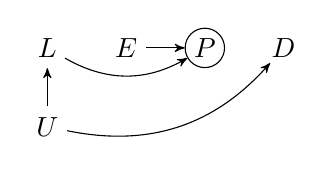
\begin{tikzpicture}[->,>=stealth',state/.style={draw,circle,minimum size=5mm, inner sep = 0pt}] 
 		\node[state,draw = none]         (L)                     {$L$};
 		\node[state,draw = none]         (U)    [below of=L]     {$U$}; 
 		\node[state,draw = none]         (E)    [right of=L]     {$E$}; 
 		\node[state,circle]              (P)    [right of=E]     {$P$}; 
 		\node[state,draw = none]         (D)    [right of=P]     {$D$}; 
 		\path (U)   edge  [bend right]   node {} (D) 
                     edge                 node {} (L) 
               (L)   edge  [bend right]   node {} (P) 
               (E)   edge                 node {} (P); 
         \end{tikzpicture} 

     \label{fig:f1a} 
 \end{subfigure} 
 \begin{subfigure}[b]{4cm} 
 	\centering 
 	\caption{}
  		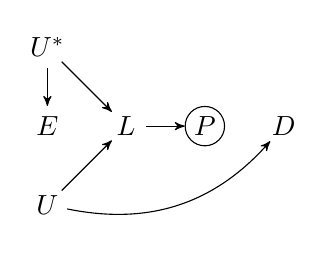
\begin{tikzpicture}[->,>=stealth',state/.style={draw,circle,minimum size=5mm, inner sep = 0pt}] 
 		\node[state,draw = none]         (Us)                    {$U^{*}$}; 
 		\node[state,draw = none]         (E)    [below of=Us]    {$E$}; 
 		\node[state,draw = none]         (U)    [below of=E]     {$U$}; 
 		\node[state,draw = none]         (L)    [right of=E]     {$L$}; 
 		\node[state,circle]              (P)    [right of=L]     {$P$}; 
 		\node[state,draw = none]         (D)    [right of=P]     {$D$}; 
 		\path (Us)  edge                 node {} (E) 
 		            edge                 node {} (L) 
 		      (U)   edge  [bend right]   node {} (D) 
 		            edge                 node {} (L) 
 		      (L)   edge                 node {} (P); 
 		\end{tikzpicture} 
 	\label{fig:f1b} 
 \end{subfigure} 
 \begin{subfigure}[b]{4cm}
 	\centering 
 	\caption{}
  		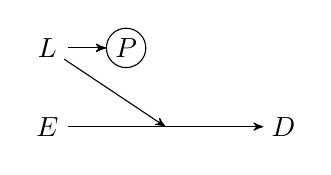
\begin{tikzpicture}[->,>=stealth',state/.style={draw,circle,minimum size=5mm, inner sep = 0pt}] 
 		\node[state,draw = none]         (L)                     {$L$};
 		\node[state,draw = none]         (E)    [below of=L]     {$E$}; 
 		\node[state,circle]              (P)    [right of=L]     {$P$}; 
 		\node[]                          (x1)   [right of=P]     {}; 
 		\node[]                          (x2)   [right of=x1]    {}; 
 		\node[state,draw = none]         (D)    [below of=x2]    {$D$}; 
 		 
 		\path (L)   edge                 node {} (P) 
 		            edge                 node {} (P) 
 		      (E)   edge                 node {} (D); 
 		       
 		\draw (L)                    --  node {} ($(E)!0.5!(D)$); 
 		\end{tikzpicture} 
 	\label{fig:f1c} 
 \end{subfigure} 

		}
	}
	
	\caption{Structural models of bias due to self-selection or loss to follow up in prospective cohort studies. A spurious association between exposure $E$ and outcome $D$ occurs when continued participation $P$ is a common effect of exposure $E$ and participation predictors $L$, and $L$ and the outcome $D$ share an unobserved common cause $U$. \protect\circled{$P$} indicates conditioning on $P$, which opens a collider \cite{Cole2010-za}, resulting in a spurious association between $D$ to $E$. Panel (a) depicts a situation where $L$ and $E$ are independent as long as there is no conditioning on $P$. This type of bias can be corrected by DS, MRP, or adjusting for $L$. (b) When $E$ and $L$ share an unobserved common cause, bias can only be corrected with IPPW. Panel (c) depicts bias due to effect modification, which can manifest in the absence of unobserved causes. It can be corrected through IPPW, DS, MRP, or by modeling the interaction between $L$ and $E$. (Panels (a) and (b) modified from \cite{Hernan2004-oz}).}
	\label{fig:SelectionBias}
\end{figure}


Figure 1 highlights that bias due to self-selection and loss to follow up depends on the relationship of variables included in an analysis with each other and with unobserved causes. Therefore, the presence or absence of bias cannot be determined for an entire cohort study that measures different exposures and outcomes. Instead, it has to be determined for each exposure-outcome-pair. Acquiring information about associations that determine selection bias is non-trivial, because \emph{unobserved} common causes of participation predictors and outcome are central. Common causes can be of environmental \cite{Johnson2011-wi,Verweij2013-xk} or genetic nature. Genetic correlation coefficients ($r_G$) from twin\cite{Tambs2012-km} or genome wide association studies \cite{Bulik-Sullivan2015-er}, which can serve as indicators of common genetic causes, are more widely reported. For instance, single nucleotide polymorphism (SNP) based genetic correlations of $r_{G_{SNP}}=0.01$ and $r_{G_{SNP}}=0.731$ between education and birth-weight or childhood IQ, respectively, were reported \cite{Bulik-Sullivan2015-xn}. Hence, if one uses a study sample that over-represents well-educated mothers to examine associations between maternal depression and birth weight or childhood IQ, the latter association is more likely biased.

A limitation of the structural approach is that it provides no estimate of selection bias--magnitude. Still, the comparison of associations estimates obtained with and without correction for self-selection into continued participation can serve as a lower bound estimate of bias. Selection bias can be reduced by adjusting for participation predictors (adjusted regression, AR), by direct standardization with respect to participation predictors (DS \cite{Miettinen1972-vf}) or multilevel regression and poststratification (MRP \cite{Downes2018-oa}), and by weighting participants according to the inverse participation-probability (IPPW \cite{Seaman2013-rj}). While IPPW reduces all types of selection bias displayed in Figure \ref{fig:SelectionBias} (provided participation can be predicted well), DS and MRP reduce bias due to effect modification and structural bias when the exposure does not cause or share a common cause with participation predictors (as in Figures \ref{fig:f1a} and \ref{fig:f1c}). AR only reduces bias when the exposure does not cause or share a common cause with participation predictors (as in Figure \ref{fig:f1a}). AR, DS, and MRP cannot reduce selection bias when the exposure causes or shares a common cause with participation predictors (as in Figure \ref{fig:f1b}) because conditioning on a collider introduces bias \cite{Cole2010-za}.

In sum, this article proposes to evaluate selection bias in two steps. First, assumptions about common causes in causal models of exposure outcome association and study participation can be substantiated with estimates of genetic correlations. Second, a lower bound of selection bias magnitude can be estimated by comparing association estimates from IPPW and non-weighted analyses. In the remainder of the article we use the association between parental characteristics and preschoolers' ADHD symptoms in the Norwegian Mother and Child Cohort study (MoBa) as an example to demonstrate assessment of bias due to self-selection and loss to follow up in a large prospective cohort study. We estimate the joint effects of self-selection and loss to follow up by assessing bias in the study population for which outcome data is available, because both biases are present in longitudinal studies. \emph{Note that in the remainder of the article "bias" refers exclusively to bias due to self-selection and loss to follow up, and not to any other type of bias.}

\section{Methods}

\subsection{Study population and study sample}

\paragraph{Study sample} MoBa is a prospective population-based pregnancy cohort study conducted by the Norwegian Institute of Public Health  \cite{Magnus2006-jj,Magnus2016-ht}. Participating mothers from all over Norway were recruited during routine ultrasound assessment in week 17 or 18 of their pregnancy in the period from 1999 to 2009. 41\% of the invited women consented to participation. MoBa participants received questionnaires in gestational week 17 or 18, week 22 and week 30, at child's age 6 and 18 months, 3, 5, and 8 years and onward. The study is still ongoing. The reported analyses also use information from the Medical Birth Registry of Norway (MBRN) \cite{Irgens2000-ra}.

The current analysis uses data from the main inclusion period from January 2001 to December 2009, in which 94373 mothers returned the first MoBa questionnaire around the 20th pregnancy week. Of these 55763 (59\%) also returned the 6th MoBa questionnaire (at child age 3 years). Table \ref{table:age_edu} shows age and education of the MoBa sample and the study population, i.e. women in Norway who gave birth in the sampling period.

\begin{table}[ht]
	\ifthenelse{\boolean{ismanus}}{}{% latex table generated in R 3.3.1 by xtable 1.8-2 package
% Mon Mar 20 10:07:03 2017

\centering
\begin{tabular}{lllrrrrrr}
  \hline
group & Education & $<$20 & 20-24 & 25-29 & 30-34 & 35-39 & 40-49 & All \\ 
  \hline
MoBa & Elementary & 0.2 & 0.40 & 0.40 & 0.40 & 0.20 & 0.10 & 1.70 \\ 
   & High-school & 0.3 & 6.20 & 9.90 & 8.70 & 4.10 & 0.60 & 29.90 \\ 
   & Bachelor & 0 & 1.80 & 16.70 & 18.00 & 6.30 & 0.80 & 43.60 \\ 
   & Master & 0 & 0.10 & 6.00 & 12.80 & 5.30 & 0.60 & 24.80 \\ 
   & All & 0.6 & 8.50 & 33.10 & 39.90 & 15.90 & 2.10 & 100.00 \\ 
  Population & Elementary & 2 & 5.60 & 5.10 & 3.70 & 1.90 & 0.50 & 18.70 \\ 
   & High-school & 0.3 & 6.80 & 11.90 & 10.30 & 4.60 & 0.80 & 34.70 \\ 
   & Bachelor & 0 & 1.90 & 13.10 & 15.00 & 6.20 & 1.00 & 37.20 \\ 
   & Master & 0 & 0.00 & 1.90 & 4.70 & 2.30 & 0.40 & 9.40 \\ 
   & All & 2.3 & 14.40 & 32.00 & 33.70 & 15.00 & 2.50 & 100.00 \\ 
  Coverage & Elementary & 1.3 & 0.70 & 1.00 & 1.30 & 1.30 & 1.30 & 1.00 \\ 
   & High-school & 12.3 & 10.30 & 9.40 & 9.50 & 10.10 & 9.10 & 9.70 \\ 
   & Bachelor & - & 10.50 & 14.30 & 13.50 & 11.40 & 9.30 & 13.20 \\ 
   & Master & - & 17.40 & 35.10 & 30.40 & 25.70 & 19.50 & 29.70 \\ 
   & All & 2.8 & 6.60 & 11.60 & 13.30 & 11.90 & 9.30 & 11.30 \\ 
   \hline
\end{tabular}
\caption{Proportion of mothers split by age and education in study sample (n = 57478) and background population (n = 510556), as well as coverage (\% participation) of population subgroups in Moba. Data for MoBa participants from MoBa and MBRN, population data were obtained from Statistics Norway. While around 30\% of mothers with a Masters degree participated, only around 1\% of mothers with only elementary school education or less participated.} 

}
	\caption{Proportion of mothers split by age and education in study sample (n = 57478) and background population (n = 510556), as well as coverage (\% participation) of population subgroups in Moba. Data for MoBa participants from MoBa and MBRN, population data were obtained from Statistics Norway. While around 30\% of mothers with a Masters degree participated, only around 1\% of mothers with only elementary school education or less participated.} 
	\label{table:age_edu}
\end{table}

\paragraph{Socioeconomic data about the study population}
We obtained aggregated data about age, educational level, and number of children for all women who became mothers in the sampling period from Statistics Norway. 


\subsection{Statistical analysis}
R scripts for all analyses are available at {\footnotesize https://github.com/gbiele/IPW/tree/master/AnalysisBIPW} and a detailed description of the statistical methods is provided in the supplementary information.

\paragraph{Investigating unobserved common causes with LD score regression} We calculated genetic correlations between predictors of participation, exposures, and outcome from publicly available summary results of genome wide association studies (GWAS) using linkage disequilibrium (LD) score regressions \cite{Bulik-Sullivan2015-er}. Table \ref{tab:gwas} lists phenotypes for which we obtained GWAS summary statistics. Genetic correlations provide information about common causes of maternal characteristics and child phenotypes because mothers and their children share 50\% of their genes.

\paragraph{Outcome, exposures, and control variables} We calculated the outcome variable "ADHD symptom score" by summing the responses (Not, Somewhat or Very often true, coded as 0, 1, 2) to 11 questions about ADHD symptoms that mothers' answered when the child was around 3 years old. Three separate analyses examined the magnitude of selection bias when estimating the effect of (a) birth-related exposures, (b) maternal and paternal use of legal drugs, and (c) maternal and paternal mental health and use of illegal drugs on preschoolers' ADHD score. Table \ref{table:variables} describes the variables used in the analyses. 

Mothers\textquotesingle \space mental health was measured as sum scores of the short forms of the symptom check list (SCL5) \cite{Tambs1993-ch} and the lifetime history of depression questionnaire (LTH) \cite{Kendler1993-pf}. Use of illegal drugs (cannabis, ecstasy, amphetamines, cocaine) before or in the pregnancy was assessed with Likert scales (less than 0.01\% indicated to having used heroin). Ability scores resulting from an item response theory analysis of these variables \cite{Rizopoulos2006-bc} were used as predictors in the regression analysis. 


\begin{table}[ht]
	\centering
	\ifthenelse{\boolean{ismanus}}{}{\input{tables/variables}}
	\caption{Description of variables.
		\newline Q6 = MoBa questionnaire at child age 3, Q1 =  MoBa questionnaire at pregnancy week 20, F = Moba fathers' questionnaire (week 20), MBRN = Medical Birth Registry of Norway, SS = sum score. SGA = small for gestational age. Mothers' smoking and drinking behavior refers to the first 20 weeks of the pregnancy. 
		\newline Outcome = outcome variable, Birth = Birth related exposures, Mental health = exposures related to mothers' and father's mental health, Legal Drugs = exposures from drinking and smoking, control = adjustment variables, Pred.part./ctrl. = predictors of participation (control variables in non-weighted analyses).
		Variable names starting with m refer to mothers, f refers to fathers, and c refers to children. All continuous and count variables except parity were re-scaled to have a mean of zero and a standard deviation of one.} 
	\label{table:variables}
\end{table}


All presented analyses used participants for which at least 50 \% of the analysis variables were available. We created 20 multiply imputed data sets with the R package mi \cite{Su2011-he}. 

\paragraph{Regression model and bias estimation}

In brief, the analysis involves simultaneous Bayesian estimation of parameters for a regression model with inverse probability of participation weighting (IPPW) and an adjusted regression (AR) model, where the AR model adjusts for the participation predictors used in the selection model. To account for covariation of regression weights, weights for the AR model are defined as  weights for the IPPW model plus a difference term. Because ADHD sum scores are constraint to be between 0 and 22 and characterized by overdispersion, we used a beta binomial regression model and report results as average marginal effects (AMEs). 


We calculated stabilized inverse probability weights using tabulated data about education, age and number of children of all birth giving mothers in Norway in the sampling period of MoBa. Because we rely on tabulated data, we used a binomial regression to estimate participation probabilities for population subgroups. We used a hierarchical regression with random intercepts and slopes for the effect of age in subgroups defined by education and parity, in order to reliably estimate effects of age also in small sub-groups (c.f. Figure \ref{fig:IPW}).


All analyses used the same set of control variables (c.f. Table \ref{table:variables}) except that only the AR analysis adjusted for participation predictors.

We calculated the lower bound bias by dividing the difference between the AME estimates of the IPPW and AR models with either the standard deviation or the mean of the IPPW estimate. Both approaches were used previously \cite{Stuart2010-cj,Nilsen2009-ci}. The former appeals to the intuition that bias is problematic if the true parameter is known with high certainty, whereas the latter appeals to the intuition that bias is problematic if it has a large deviation from the true parameter. To test for bias, we check how much of the posterior distribution of the bias lies within a region of practical equivalence (ROPE), i.e. a bias magnitude that is for practical purposes equivalent with zero \cite{Kruschke2010-zi, Mascha2011-um}. This also allows quantifying the risk for substantial bias as the ratio of the posterior probabilities of the lower bound bias estimate being inside and outside the ROPE. Similar to earlier research, which defined deviations of larger than 30 or 40\% of the standard deviation or mean of comparison standard as problematic \cite{Stuart2010-cj,Nohr2006-uf}, we define biases of less than 0.5 as practically equivalent with zero. To obtain a simple measure of risk for bias we calculate the the ratio of the posterior distribution mass inside and outside the ROPE, $RR_b$. For example, a $log(RR_b)$ of -1.6 means that the lower bound bias estimate is five times as likely to lie outside the ROPE.

Regression analyses were performed with custom models implemented in the probabilistic programming language Stan \cite{Stan_Development_Team2017-lp} and fit with RStan\cite{Stan_Development_Team2017-lp}.

\section{Results}

Statistics Norway recorded 510\,561 women who became mothers in the period from 2001 to 2009. In the same period, 94\,373 mothers returned the first MoBa questionnaire (Q1). Of these, 55\,763 also returned the sixth questionnaire,  which was sent out when  children were 3 years old. 54\,557 returned questionnaires with fewer than 50\% missing data among the variables of interest. The study sample used for the reported analysis constitute around 14\% of the study population.

\subsection*{Socio-demographic composition of study sample and population}
 Mothers with elementary school education or less constitute around 18.7\% of the study population but only 1.7\% of the MoBa sample (see Table \ref{table:age_edu}). 16.6\% of mothers in the study population are younger than 25, compared to around 9.1\% in the study sample. Accordingly, the participation rates vary substantially between population subgroups: 23.8\% of mothers with a master's degree participated in MoBa, but only around 0.8\% of mothers with elementary school education. For parity, the difference between MoBa and study population is less pronounced. The percentages of women in the study population (MoBa) who had previously 0, 1, 2, or 3 or more children are 41.8 (50.9), 36.3 (32.5), 16.1 (13.9), 2.8 (5.8), respectively. Hence, MoBa over-represents mothers of firstborn children and under-represents those with more than two children.

\subsection*{Inverse probability weights}
The hierarchical binomial model captured participation well, as indicated by a correlation of $r=0.99$ between modeled and observed participation rates (see Figure \ref{fig:IPW}). Mothers' education was the key variable to predict participation. Smoothed weights ranged between on average 0.31 and 21.36. The largest weights were for mothers with only elementary school education, and the smallest for mothers with a master's degree. We chose not to trim extreme weights, because this would result in improper weighting of the study sample. Note that while some weights are very large, the associated population subgroups are typically represented with more than children in the analysed MoBa study sample.

\subsection*{Unobserved genetic common causes}
Genetic correlation results indicate unobserved common causes of participation predictors and outcome or exposures, respectively (see Figure \ref{fig:rg}). For example, genes associated with "age at first birth" or "years of education" are also (negatively) associated with ADHD, maternal mental health, or smoking. The overall SNP based heritability is generally not high, and often below 10\%.

\begin{figure}
	\begin{center}
		\ifthenelse{\boolean{ismanus}}{}{% Created by tikzDevice version 0.11 on 2018-05-04 12:24:43
% !TEX encoding = UTF-8 Unicode
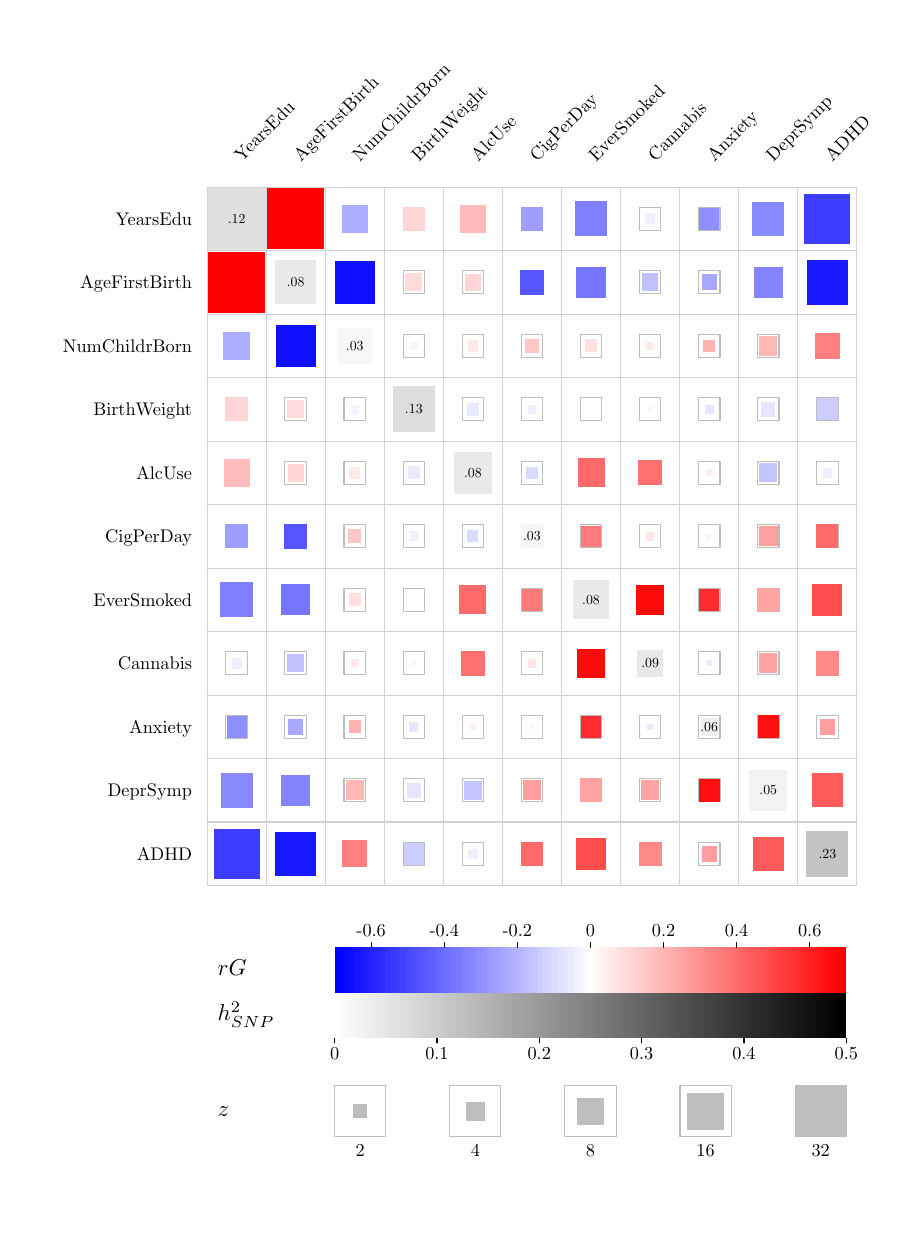
\begin{tikzpicture}[x=1pt,y=1pt]
\definecolor{fillColor}{RGB}{255,255,255}
\path[use as bounding box,fill=fillColor,fill opacity=0.00] (0,0) rectangle (312.98,426.79);
\begin{scope}
\path[clip] ( 55.44,106.70) rectangle (309.02,379.27);
\definecolor{drawColor}{RGB}{190,190,190}
\definecolor{fillColor}{RGB}{255,255,255}

\path[draw=drawColor,line width= 0.4pt,line join=round,line cap=round,fill=fillColor] (114.31,330.58) rectangle (122.08,338.94);
\definecolor{fillColor}{RGB}{15,15,255}

\path[fill=fillColor] (111.03,327.06) rectangle (125.36,342.46);
\definecolor{fillColor}{RGB}{255,255,255}

\path[draw=drawColor,line width= 0.4pt,line join=round,line cap=round,fill=fillColor] ( 92.96,307.64) rectangle (100.74,315.99);
\definecolor{fillColor}{RGB}{15,15,255}

\path[fill=fillColor] ( 89.69,304.12) rectangle (104.01,319.51);
\definecolor{fillColor}{RGB}{255,255,255}

\path[draw=drawColor,line width= 0.4pt,line join=round,line cap=round,fill=fillColor] (285.07,330.58) rectangle (292.84,338.94);
\definecolor{fillColor}{RGB}{25,25,255}

\path[fill=fillColor] (281.50,326.75) rectangle (296.41,342.77);
\definecolor{fillColor}{RGB}{255,255,255}

\path[draw=drawColor,line width= 0.4pt,line join=round,line cap=round,fill=fillColor] ( 92.96,124.09) rectangle (100.74,132.44);
\definecolor{fillColor}{RGB}{25,25,255}

\path[fill=fillColor] ( 89.39,120.25) rectangle (104.31,136.28);
\definecolor{fillColor}{RGB}{255,255,255}

\path[draw=drawColor,line width= 0.4pt,line join=round,line cap=round,fill=fillColor] (285.07,353.53) rectangle (292.84,361.88);
\definecolor{fillColor}{RGB}{61,61,255}

\path[fill=fillColor] (280.63,348.75) rectangle (297.28,366.65);
\definecolor{fillColor}{RGB}{255,255,255}

\path[draw=drawColor,line width= 0.4pt,line join=round,line cap=round,fill=fillColor] ( 71.62,124.09) rectangle ( 79.39,132.44);
\definecolor{fillColor}{RGB}{61,61,255}

\path[fill=fillColor] ( 67.18,119.31) rectangle ( 83.83,137.22);
\definecolor{fillColor}{RGB}{255,255,255}

\path[draw=drawColor,line width= 0.4pt,line join=round,line cap=round,fill=fillColor] (178.34,330.58) rectangle (186.12,338.94);
\definecolor{fillColor}{RGB}{86,86,255}

\path[fill=fillColor] (178.06,330.28) rectangle (186.40,339.24);
\definecolor{fillColor}{RGB}{255,255,255}

\path[draw=drawColor,line width= 0.4pt,line join=round,line cap=round,fill=fillColor] ( 92.96,238.81) rectangle (100.74,247.16);
\definecolor{fillColor}{RGB}{86,86,255}

\path[fill=fillColor] ( 92.68,238.50) rectangle (101.02,247.47);
\definecolor{fillColor}{RGB}{255,255,255}

\path[draw=drawColor,line width= 0.4pt,line join=round,line cap=round,fill=fillColor] (199.69,330.58) rectangle (207.46,338.94);
\definecolor{fillColor}{RGB}{117,117,255}

\path[fill=fillColor] (198.31,329.10) rectangle (208.84,340.42);
\definecolor{fillColor}{RGB}{255,255,255}

\path[draw=drawColor,line width= 0.4pt,line join=round,line cap=round,fill=fillColor] ( 92.96,215.86) rectangle (100.74,224.22);
\definecolor{fillColor}{RGB}{117,117,255}

\path[fill=fillColor] ( 91.58,214.38) rectangle (102.11,225.70);
\definecolor{fillColor}{RGB}{255,255,255}

\path[draw=drawColor,line width= 0.4pt,line join=round,line cap=round,fill=fillColor] ( 71.62,215.86) rectangle ( 79.39,224.22);
\definecolor{fillColor}{RGB}{127,127,255}

\path[fill=fillColor] ( 69.64,213.73) rectangle ( 81.37,226.35);
\definecolor{fillColor}{RGB}{255,255,255}

\path[draw=drawColor,line width= 0.4pt,line join=round,line cap=round,fill=fillColor] (199.69,353.53) rectangle (207.46,361.88);
\definecolor{fillColor}{RGB}{127,127,255}

\path[fill=fillColor] (197.71,351.40) rectangle (209.44,364.01);
\definecolor{fillColor}{RGB}{255,255,255}

\path[draw=drawColor,line width= 0.4pt,line join=round,line cap=round,fill=fillColor] (263.72,330.58) rectangle (271.50,338.94);
\definecolor{fillColor}{RGB}{132,132,255}

\path[fill=fillColor] (262.31,329.06) rectangle (272.91,340.46);
\definecolor{fillColor}{RGB}{255,255,255}

\path[draw=drawColor,line width= 0.4pt,line join=round,line cap=round,fill=fillColor] ( 92.96,147.03) rectangle (100.74,155.39);
\definecolor{fillColor}{RGB}{132,132,255}

\path[fill=fillColor] ( 91.55,145.51) rectangle (102.15,156.90);
\definecolor{fillColor}{RGB}{255,255,255}

\path[draw=drawColor,line width= 0.4pt,line join=round,line cap=round,fill=fillColor] (263.72,353.53) rectangle (271.50,361.88);
\definecolor{fillColor}{RGB}{137,137,255}

\path[fill=fillColor] (261.79,351.45) rectangle (273.43,363.96);
\definecolor{fillColor}{RGB}{255,255,255}

\path[draw=drawColor,line width= 0.4pt,line join=round,line cap=round,fill=fillColor] ( 71.62,147.03) rectangle ( 79.39,155.39);
\definecolor{fillColor}{RGB}{137,137,255}

\path[fill=fillColor] ( 69.69,144.95) rectangle ( 81.32,157.46);
\definecolor{fillColor}{RGB}{255,255,255}

\path[draw=drawColor,line width= 0.4pt,line join=round,line cap=round,fill=fillColor] (242.38,353.53) rectangle (250.15,361.88);
\definecolor{fillColor}{RGB}{142,142,255}

\path[fill=fillColor] (242.62,353.79) rectangle (249.91,361.62);
\definecolor{fillColor}{RGB}{255,255,255}

\path[draw=drawColor,line width= 0.4pt,line join=round,line cap=round,fill=fillColor] ( 71.62,169.98) rectangle ( 79.39,178.33);
\definecolor{fillColor}{RGB}{142,142,255}

\path[fill=fillColor] ( 71.86,170.24) rectangle ( 79.15,178.07);
\definecolor{fillColor}{RGB}{255,255,255}

\path[draw=drawColor,line width= 0.4pt,line join=round,line cap=round,fill=fillColor] (178.34,353.53) rectangle (186.12,361.88);
\definecolor{fillColor}{RGB}{158,158,255}

\path[fill=fillColor] (178.21,353.38) rectangle (186.25,362.03);
\definecolor{fillColor}{RGB}{255,255,255}

\path[draw=drawColor,line width= 0.4pt,line join=round,line cap=round,fill=fillColor] ( 71.62,238.81) rectangle ( 79.39,247.16);
\definecolor{fillColor}{RGB}{158,158,255}

\path[fill=fillColor] ( 71.48,238.66) rectangle ( 79.53,247.31);
\definecolor{fillColor}{RGB}{255,255,255}

\path[draw=drawColor,line width= 0.4pt,line join=round,line cap=round,fill=fillColor] (242.38,330.58) rectangle (250.15,338.94);
\definecolor{fillColor}{RGB}{168,168,255}

\path[fill=fillColor] (243.55,331.84) rectangle (248.98,337.68);
\definecolor{fillColor}{RGB}{255,255,255}

\path[draw=drawColor,line width= 0.4pt,line join=round,line cap=round,fill=fillColor] ( 92.96,169.98) rectangle (100.74,178.33);
\definecolor{fillColor}{RGB}{168,168,255}

\path[fill=fillColor] ( 94.13,171.23) rectangle ( 99.57,177.07);
\definecolor{fillColor}{RGB}{255,255,255}

\path[draw=drawColor,line width= 0.4pt,line join=round,line cap=round,fill=fillColor] ( 71.62,307.64) rectangle ( 79.39,315.99);
\definecolor{fillColor}{RGB}{173,173,255}

\path[fill=fillColor] ( 70.73,306.69) rectangle ( 80.28,316.95);
\definecolor{fillColor}{RGB}{255,255,255}

\path[draw=drawColor,line width= 0.4pt,line join=round,line cap=round,fill=fillColor] (114.31,353.53) rectangle (122.08,361.88);
\definecolor{fillColor}{RGB}{173,173,255}

\path[fill=fillColor] (113.42,352.57) rectangle (122.97,362.83);
\definecolor{fillColor}{RGB}{255,255,255}

\path[draw=drawColor,line width= 0.4pt,line join=round,line cap=round,fill=fillColor] (221.03,330.58) rectangle (228.81,338.94);
\definecolor{fillColor}{RGB}{193,193,255}

\path[fill=fillColor] (221.94,331.56) rectangle (227.90,337.96);
\definecolor{fillColor}{RGB}{255,255,255}

\path[draw=drawColor,line width= 0.4pt,line join=round,line cap=round,fill=fillColor] ( 92.96,192.92) rectangle (100.74,201.27);
\definecolor{fillColor}{RGB}{193,193,255}

\path[fill=fillColor] ( 93.87,193.89) rectangle ( 99.83,200.30);
\definecolor{fillColor}{RGB}{255,255,255}

\path[draw=drawColor,line width= 0.4pt,line join=round,line cap=round,fill=fillColor] (157.00,147.03) rectangle (164.77,155.39);
\definecolor{fillColor}{RGB}{198,198,255}

\path[fill=fillColor] (157.66,147.74) rectangle (164.11,154.68);
\definecolor{fillColor}{RGB}{255,255,255}

\path[draw=drawColor,line width= 0.4pt,line join=round,line cap=round,fill=fillColor] (263.72,261.75) rectangle (271.50,270.11);
\definecolor{fillColor}{RGB}{198,198,255}

\path[fill=fillColor] (264.38,262.46) rectangle (270.84,269.40);
\definecolor{fillColor}{RGB}{255,255,255}

\path[draw=drawColor,line width= 0.4pt,line join=round,line cap=round,fill=fillColor] (285.07,284.70) rectangle (292.84,293.05);
\definecolor{fillColor}{RGB}{204,204,255}

\path[fill=fillColor] (285.28,284.92) rectangle (292.63,292.82);
\definecolor{fillColor}{RGB}{255,255,255}

\path[draw=drawColor,line width= 0.4pt,line join=round,line cap=round,fill=fillColor] (135.65,124.09) rectangle (143.43,132.44);
\definecolor{fillColor}{RGB}{204,204,255}

\path[fill=fillColor] (135.86,124.31) rectangle (143.22,132.22);
\definecolor{fillColor}{RGB}{255,255,255}

\path[draw=drawColor,line width= 0.4pt,line join=round,line cap=round,fill=fillColor] (157.00,238.81) rectangle (164.77,247.16);
\definecolor{fillColor}{RGB}{219,219,255}

\path[fill=fillColor] (158.87,240.82) rectangle (162.90,245.15);
\definecolor{fillColor}{RGB}{255,255,255}

\path[draw=drawColor,line width= 0.4pt,line join=round,line cap=round,fill=fillColor] (178.34,261.75) rectangle (186.12,270.11);
\definecolor{fillColor}{RGB}{219,219,255}

\path[fill=fillColor] (180.22,263.77) rectangle (184.24,268.09);
\definecolor{fillColor}{RGB}{255,255,255}

\path[draw=drawColor,line width= 0.4pt,line join=round,line cap=round,fill=fillColor] (135.65,169.98) rectangle (143.43,178.33);
\definecolor{fillColor}{RGB}{229,229,255}

\path[fill=fillColor] (137.96,172.46) rectangle (141.12,175.85);
\definecolor{fillColor}{RGB}{255,255,255}

\path[draw=drawColor,line width= 0.4pt,line join=round,line cap=round,fill=fillColor] (135.65,147.03) rectangle (143.43,155.39);
\definecolor{fillColor}{RGB}{229,229,255}

\path[fill=fillColor] (137.01,148.49) rectangle (142.07,153.93);
\definecolor{fillColor}{RGB}{255,255,255}

\path[draw=drawColor,line width= 0.4pt,line join=round,line cap=round,fill=fillColor] (242.38,284.70) rectangle (250.15,293.05);
\definecolor{fillColor}{RGB}{229,229,255}

\path[fill=fillColor] (244.69,287.17) rectangle (247.84,290.57);
\definecolor{fillColor}{RGB}{255,255,255}

\path[draw=drawColor,line width= 0.4pt,line join=round,line cap=round,fill=fillColor] (263.72,284.70) rectangle (271.50,293.05);
\definecolor{fillColor}{RGB}{229,229,255}

\path[fill=fillColor] (265.08,286.16) rectangle (270.14,291.59);
\definecolor{fillColor}{RGB}{255,255,255}

\path[draw=drawColor,line width= 0.4pt,line join=round,line cap=round,fill=fillColor] (157.00,284.70) rectangle (164.77,293.05);
\definecolor{fillColor}{RGB}{234,234,255}

\path[fill=fillColor] (158.65,286.47) rectangle (163.12,291.28);
\definecolor{fillColor}{RGB}{255,255,255}

\path[draw=drawColor,line width= 0.4pt,line join=round,line cap=round,fill=fillColor] (221.03,169.98) rectangle (228.81,178.33);
\definecolor{fillColor}{RGB}{234,234,255}

\path[fill=fillColor] (223.88,173.04) rectangle (225.96,175.27);
\definecolor{fillColor}{RGB}{255,255,255}

\path[draw=drawColor,line width= 0.4pt,line join=round,line cap=round,fill=fillColor] (135.65,261.75) rectangle (143.43,270.11);
\definecolor{fillColor}{RGB}{234,234,255}

\path[fill=fillColor] (137.30,263.52) rectangle (141.78,268.34);
\definecolor{fillColor}{RGB}{255,255,255}

\path[draw=drawColor,line width= 0.4pt,line join=round,line cap=round,fill=fillColor] (242.38,192.92) rectangle (250.15,201.27);
\definecolor{fillColor}{RGB}{234,234,255}

\path[fill=fillColor] (245.23,195.98) rectangle (247.30,198.21);
\definecolor{fillColor}{RGB}{255,255,255}

\path[draw=drawColor,line width= 0.4pt,line join=round,line cap=round,fill=fillColor] (157.00,124.09) rectangle (164.77,132.44);
\definecolor{fillColor}{RGB}{239,239,255}

\path[fill=fillColor] (159.20,126.45) rectangle (162.57,130.08);
\definecolor{fillColor}{RGB}{255,255,255}

\path[draw=drawColor,line width= 0.4pt,line join=round,line cap=round,fill=fillColor] (221.03,353.53) rectangle (228.81,361.88);
\definecolor{fillColor}{RGB}{239,239,255}

\path[fill=fillColor] (223.09,355.73) rectangle (226.75,359.68);
\definecolor{fillColor}{RGB}{255,255,255}

\path[draw=drawColor,line width= 0.4pt,line join=round,line cap=round,fill=fillColor] (178.34,284.70) rectangle (186.12,293.05);
\definecolor{fillColor}{RGB}{239,239,255}

\path[fill=fillColor] (180.61,287.13) rectangle (183.85,290.62);
\definecolor{fillColor}{RGB}{255,255,255}

\path[draw=drawColor,line width= 0.4pt,line join=round,line cap=round,fill=fillColor] (285.07,261.75) rectangle (292.84,270.11);
\definecolor{fillColor}{RGB}{239,239,255}

\path[fill=fillColor] (287.27,264.11) rectangle (290.65,267.74);
\definecolor{fillColor}{RGB}{255,255,255}

\path[draw=drawColor,line width= 0.4pt,line join=round,line cap=round,fill=fillColor] ( 71.62,192.92) rectangle ( 79.39,201.27);
\definecolor{fillColor}{RGB}{239,239,255}

\path[fill=fillColor] ( 73.67,195.13) rectangle ( 77.34,199.07);
\definecolor{fillColor}{RGB}{255,255,255}

\path[draw=drawColor,line width= 0.4pt,line join=round,line cap=round,fill=fillColor] (135.65,238.81) rectangle (143.43,247.16);
\definecolor{fillColor}{RGB}{239,239,255}

\path[fill=fillColor] (137.92,241.24) rectangle (141.16,244.73);
\definecolor{fillColor}{RGB}{255,255,255}

\path[draw=drawColor,line width= 0.4pt,line join=round,line cap=round,fill=fillColor] (135.65,307.64) rectangle (143.43,315.99);
\definecolor{fillColor}{RGB}{244,244,255}

\path[fill=fillColor] (138.12,310.29) rectangle (140.96,313.35);
\definecolor{fillColor}{RGB}{255,255,255}

\path[draw=drawColor,line width= 0.4pt,line join=round,line cap=round,fill=fillColor] (178.34,169.98) rectangle (186.12,178.33);
\definecolor{fillColor}{RGB}{244,244,255}

\path[fill=fillColor] (181.47,173.33) rectangle (182.99,174.97);
\definecolor{fillColor}{RGB}{255,255,255}

\path[draw=drawColor,line width= 0.4pt,line join=round,line cap=round,fill=fillColor] (114.31,284.70) rectangle (122.08,293.05);
\definecolor{fillColor}{RGB}{244,244,255}

\path[fill=fillColor] (116.77,287.34) rectangle (119.62,290.40);
\definecolor{fillColor}{RGB}{255,255,255}

\path[draw=drawColor,line width= 0.4pt,line join=round,line cap=round,fill=fillColor] (242.38,238.81) rectangle (250.15,247.16);
\definecolor{fillColor}{RGB}{244,244,255}

\path[fill=fillColor] (245.50,242.16) rectangle (247.03,243.81);
\definecolor{fillColor}{RGB}{255,255,255}

\path[draw=drawColor,line width= 0.4pt,line join=round,line cap=round,fill=fillColor] (221.03,284.70) rectangle (228.81,293.05);
\definecolor{fillColor}{RGB}{249,249,255}

\path[fill=fillColor] (223.94,287.82) rectangle (225.90,289.92);
\definecolor{fillColor}{RGB}{255,255,255}

\path[draw=drawColor,line width= 0.4pt,line join=round,line cap=round,fill=fillColor] (135.65,192.92) rectangle (143.43,201.27);
\definecolor{fillColor}{RGB}{249,249,255}

\path[fill=fillColor] (138.56,196.04) rectangle (140.52,198.15);
\definecolor{fillColor}{RGB}{255,255,255}

\path[draw=drawColor,line width= 0.4pt,line join=round,line cap=round,fill=fillColor] (135.65,215.86) rectangle (143.43,224.22);

\path[fill=fillColor] (138.79,219.23) rectangle (140.29,220.85);

\path[draw=drawColor,line width= 0.4pt,line join=round,line cap=round,fill=fillColor] (199.69,284.70) rectangle (207.46,293.05);

\path[fill=fillColor] (202.82,288.07) rectangle (204.33,289.68);

\path[draw=drawColor,line width= 0.4pt,line join=round,line cap=round,fill=fillColor] (178.34,238.81) rectangle (186.12,247.16);
\definecolor{fillColor}{gray}{0.97}

\path[fill=fillColor] (178.19,238.64) rectangle (186.27,247.32);
\definecolor{drawColor}{RGB}{0,0,0}

\node[text=drawColor,anchor=base,inner sep=0pt, outer sep=0pt, scale=  0.50] at (182.23,241.40) {.03};
\definecolor{drawColor}{RGB}{190,190,190}
\definecolor{fillColor}{RGB}{255,255,255}

\path[draw=drawColor,line width= 0.4pt,line join=round,line cap=round,fill=fillColor] (114.31,307.64) rectangle (122.08,315.99);
\definecolor{fillColor}{gray}{0.97}

\path[fill=fillColor] (112.07,305.23) rectangle (124.32,318.40);
\definecolor{drawColor}{RGB}{0,0,0}

\node[text=drawColor,anchor=base,inner sep=0pt, outer sep=0pt, scale=  0.50] at (118.19,310.23) {.03};
\definecolor{drawColor}{RGB}{190,190,190}
\definecolor{fillColor}{RGB}{255,255,255}

\path[draw=drawColor,line width= 0.4pt,line join=round,line cap=round,fill=fillColor] (157.00,169.98) rectangle (164.77,178.33);
\definecolor{fillColor}{RGB}{255,239,239}

\path[fill=fillColor] (159.68,172.86) rectangle (162.09,175.45);
\definecolor{fillColor}{RGB}{255,255,255}

\path[draw=drawColor,line width= 0.4pt,line join=round,line cap=round,fill=fillColor] (242.38,261.75) rectangle (250.15,270.11);
\definecolor{fillColor}{RGB}{255,239,239}

\path[fill=fillColor] (245.06,264.63) rectangle (247.47,267.22);
\definecolor{fillColor}{RGB}{255,255,255}

\path[draw=drawColor,line width= 0.4pt,line join=round,line cap=round,fill=fillColor] (263.72,147.03) rectangle (271.50,155.39);
\definecolor{fillColor}{gray}{0.95}

\path[fill=fillColor] (260.67,143.75) rectangle (274.55,158.67);
\definecolor{drawColor}{RGB}{0,0,0}

\node[text=drawColor,anchor=base,inner sep=0pt, outer sep=0pt, scale=  0.50] at (267.61,149.62) {.05};
\definecolor{drawColor}{RGB}{190,190,190}
\definecolor{fillColor}{RGB}{255,255,255}

\path[draw=drawColor,line width= 0.4pt,line join=round,line cap=round,fill=fillColor] (221.03,307.64) rectangle (228.81,315.99);
\definecolor{fillColor}{RGB}{255,234,234}

\path[fill=fillColor] (223.51,310.31) rectangle (226.33,313.33);
\definecolor{fillColor}{RGB}{255,255,255}

\path[draw=drawColor,line width= 0.4pt,line join=round,line cap=round,fill=fillColor] (114.31,192.92) rectangle (122.08,201.27);
\definecolor{fillColor}{RGB}{255,234,234}

\path[fill=fillColor] (116.79,195.59) rectangle (119.60,198.61);
\definecolor{fillColor}{RGB}{255,255,255}

\path[draw=drawColor,line width= 0.4pt,line join=round,line cap=round,fill=fillColor] (157.00,307.64) rectangle (164.77,315.99);
\definecolor{fillColor}{RGB}{255,234,234}

\path[fill=fillColor] (158.95,309.73) rectangle (162.82,313.90);
\definecolor{fillColor}{RGB}{255,255,255}

\path[draw=drawColor,line width= 0.4pt,line join=round,line cap=round,fill=fillColor] (114.31,261.75) rectangle (122.08,270.11);
\definecolor{fillColor}{RGB}{255,234,234}

\path[fill=fillColor] (116.26,263.84) rectangle (120.13,268.01);
\definecolor{fillColor}{RGB}{255,255,255}

\path[draw=drawColor,line width= 0.4pt,line join=round,line cap=round,fill=fillColor] (242.38,169.98) rectangle (250.15,178.33);
\definecolor{fillColor}{RGB}{239,239,239}

\path[fill=fillColor] (243.18,170.83) rectangle (249.35,177.47);
\definecolor{drawColor}{RGB}{0,0,0}

\node[text=drawColor,anchor=base,inner sep=0pt, outer sep=0pt, scale=  0.50] at (246.27,172.57) {.06};
\definecolor{drawColor}{RGB}{190,190,190}
\definecolor{fillColor}{RGB}{255,255,255}

\path[draw=drawColor,line width= 0.4pt,line join=round,line cap=round,fill=fillColor] (221.03,238.81) rectangle (228.81,247.16);
\definecolor{fillColor}{RGB}{255,229,229}

\path[fill=fillColor] (223.45,241.40) rectangle (226.39,244.56);
\definecolor{fillColor}{RGB}{255,255,255}

\path[draw=drawColor,line width= 0.4pt,line join=round,line cap=round,fill=fillColor] (178.34,192.92) rectangle (186.12,201.27);
\definecolor{fillColor}{RGB}{255,229,229}

\path[fill=fillColor] (180.76,195.52) rectangle (183.70,198.68);
\definecolor{fillColor}{RGB}{255,255,255}

\path[draw=drawColor,line width= 0.4pt,line join=round,line cap=round,fill=fillColor] (199.69,215.86) rectangle (207.46,224.22);
\definecolor{fillColor}{RGB}{234,234,234}

\path[fill=fillColor] (197.01,212.99) rectangle (210.14,227.10);
\definecolor{drawColor}{RGB}{0,0,0}

\node[text=drawColor,anchor=base,inner sep=0pt, outer sep=0pt, scale=  0.50] at (203.58,218.45) {.08};
\definecolor{drawColor}{RGB}{190,190,190}
\definecolor{fillColor}{RGB}{255,255,255}

\path[draw=drawColor,line width= 0.4pt,line join=round,line cap=round,fill=fillColor] (199.69,307.64) rectangle (207.46,315.99);
\definecolor{fillColor}{RGB}{255,224,224}

\path[fill=fillColor] (201.38,309.45) rectangle (205.77,314.18);
\definecolor{fillColor}{RGB}{255,255,255}

\path[draw=drawColor,line width= 0.4pt,line join=round,line cap=round,fill=fillColor] (114.31,215.86) rectangle (122.08,224.22);
\definecolor{fillColor}{RGB}{255,224,224}

\path[fill=fillColor] (116.00,217.68) rectangle (120.39,222.40);
\definecolor{fillColor}{RGB}{255,255,255}

\path[draw=drawColor,line width= 0.4pt,line join=round,line cap=round,fill=fillColor] ( 92.96,330.58) rectangle (100.74,338.94);
\definecolor{fillColor}{RGB}{234,234,234}

\path[fill=fillColor] ( 89.43,326.79) rectangle (104.27,342.73);
\definecolor{drawColor}{RGB}{0,0,0}

\node[text=drawColor,anchor=base,inner sep=0pt, outer sep=0pt, scale=  0.50] at ( 96.85,333.17) {.08};
\definecolor{drawColor}{RGB}{190,190,190}
\definecolor{fillColor}{RGB}{255,255,255}

\path[draw=drawColor,line width= 0.4pt,line join=round,line cap=round,fill=fillColor] (157.00,261.75) rectangle (164.77,270.11);
\definecolor{fillColor}{RGB}{234,234,234}

\path[fill=fillColor] (153.89,258.41) rectangle (167.88,273.45);
\definecolor{drawColor}{RGB}{0,0,0}

\node[text=drawColor,anchor=base,inner sep=0pt, outer sep=0pt, scale=  0.50] at (160.89,264.34) {.08};
\definecolor{drawColor}{RGB}{190,190,190}
\definecolor{fillColor}{RGB}{255,255,255}

\path[draw=drawColor,line width= 0.4pt,line join=round,line cap=round,fill=fillColor] (221.03,192.92) rectangle (228.81,201.27);
\definecolor{fillColor}{gray}{0.91}

\path[fill=fillColor] (220.35,192.18) rectangle (229.49,202.01);
\definecolor{drawColor}{RGB}{0,0,0}

\node[text=drawColor,anchor=base,inner sep=0pt, outer sep=0pt, scale=  0.50] at (224.92,195.51) {.09};
\definecolor{drawColor}{RGB}{190,190,190}
\definecolor{fillColor}{RGB}{255,255,255}

\path[draw=drawColor,line width= 0.4pt,line join=round,line cap=round,fill=fillColor] (135.65,330.58) rectangle (143.43,338.94);
\definecolor{fillColor}{RGB}{255,219,219}

\path[fill=fillColor] (136.47,331.46) rectangle (142.61,338.06);
\definecolor{fillColor}{RGB}{255,255,255}

\path[draw=drawColor,line width= 0.4pt,line join=round,line cap=round,fill=fillColor] ( 92.96,284.70) rectangle (100.74,293.05);
\definecolor{fillColor}{RGB}{255,219,219}

\path[fill=fillColor] ( 93.78,285.57) rectangle ( 99.92,292.18);
\definecolor{fillColor}{RGB}{255,255,255}

\path[draw=drawColor,line width= 0.4pt,line join=round,line cap=round,fill=fillColor] (157.00,330.58) rectangle (164.77,338.94);
\definecolor{fillColor}{RGB}{255,214,214}

\path[fill=fillColor] (157.93,331.58) rectangle (163.84,337.94);
\definecolor{fillColor}{RGB}{255,255,255}

\path[draw=drawColor,line width= 0.4pt,line join=round,line cap=round,fill=fillColor] (135.65,353.53) rectangle (143.43,361.88);
\definecolor{fillColor}{RGB}{255,214,214}

\path[fill=fillColor] (135.49,353.35) rectangle (143.59,362.06);
\definecolor{fillColor}{RGB}{255,255,255}

\path[draw=drawColor,line width= 0.4pt,line join=round,line cap=round,fill=fillColor] ( 92.96,261.75) rectangle (100.74,270.11);
\definecolor{fillColor}{RGB}{255,214,214}

\path[fill=fillColor] ( 93.89,262.75) rectangle ( 99.81,269.11);
\definecolor{fillColor}{RGB}{255,255,255}

\path[draw=drawColor,line width= 0.4pt,line join=round,line cap=round,fill=fillColor] ( 71.62,284.70) rectangle ( 79.39,293.05);
\definecolor{fillColor}{RGB}{255,214,214}

\path[fill=fillColor] ( 71.45,284.52) rectangle ( 79.56,293.23);
\definecolor{fillColor}{RGB}{255,255,255}

\path[draw=drawColor,line width= 0.4pt,line join=round,line cap=round,fill=fillColor] ( 71.62,353.53) rectangle ( 79.39,361.88);
\definecolor{fillColor}{gray}{0.88}

\path[fill=fillColor] ( 64.83,346.23) rectangle ( 86.18,369.18);
\definecolor{drawColor}{RGB}{0,0,0}

\node[text=drawColor,anchor=base,inner sep=0pt, outer sep=0pt, scale=  0.50] at ( 75.50,356.12) {.12};
\definecolor{drawColor}{RGB}{190,190,190}
\definecolor{fillColor}{RGB}{255,255,255}

\path[draw=drawColor,line width= 0.4pt,line join=round,line cap=round,fill=fillColor] (135.65,284.70) rectangle (143.43,293.05);
\definecolor{fillColor}{RGB}{221,221,221}

\path[fill=fillColor] (131.84,280.60) rectangle (147.24,297.15);
\definecolor{drawColor}{RGB}{0,0,0}

\node[text=drawColor,anchor=base,inner sep=0pt, outer sep=0pt, scale=  0.50] at (139.54,287.28) {.13};
\definecolor{drawColor}{RGB}{190,190,190}
\definecolor{fillColor}{RGB}{255,255,255}

\path[draw=drawColor,line width= 0.4pt,line join=round,line cap=round,fill=fillColor] (178.34,307.64) rectangle (186.12,315.99);
\definecolor{fillColor}{RGB}{255,198,198}

\path[fill=fillColor] (179.85,309.26) rectangle (184.61,314.38);
\definecolor{fillColor}{RGB}{255,255,255}

\path[draw=drawColor,line width= 0.4pt,line join=round,line cap=round,fill=fillColor] (114.31,238.81) rectangle (122.08,247.16);
\definecolor{fillColor}{RGB}{255,198,198}

\path[fill=fillColor] (115.81,240.43) rectangle (120.58,245.54);
\definecolor{fillColor}{RGB}{255,255,255}

\path[draw=drawColor,line width= 0.4pt,line join=round,line cap=round,fill=fillColor] (157.00,353.53) rectangle (164.77,361.88);
\definecolor{fillColor}{RGB}{255,188,188}

\path[fill=fillColor] (156.18,352.64) rectangle (165.59,362.76);
\definecolor{fillColor}{RGB}{255,255,255}

\path[draw=drawColor,line width= 0.4pt,line join=round,line cap=round,fill=fillColor] ( 71.62,261.75) rectangle ( 79.39,270.11);
\definecolor{fillColor}{RGB}{255,188,188}

\path[fill=fillColor] ( 70.80,260.87) rectangle ( 80.21,270.99);
\definecolor{fillColor}{RGB}{255,255,255}

\path[draw=drawColor,line width= 0.4pt,line join=round,line cap=round,fill=fillColor] (263.72,307.64) rectangle (271.50,315.99);
\definecolor{fillColor}{RGB}{255,183,183}

\path[fill=fillColor] (264.30,308.25) rectangle (270.92,315.38);
\definecolor{fillColor}{RGB}{255,255,255}

\path[draw=drawColor,line width= 0.4pt,line join=round,line cap=round,fill=fillColor] (114.31,147.03) rectangle (122.08,155.39);
\definecolor{fillColor}{RGB}{255,183,183}

\path[fill=fillColor] (114.88,147.65) rectangle (121.51,154.77);
\definecolor{fillColor}{RGB}{255,255,255}

\path[draw=drawColor,line width= 0.4pt,line join=round,line cap=round,fill=fillColor] (242.38,307.64) rectangle (250.15,315.99);
\definecolor{fillColor}{RGB}{255,178,178}

\path[fill=fillColor] (244.14,309.53) rectangle (248.39,314.10);
\definecolor{fillColor}{RGB}{255,255,255}

\path[draw=drawColor,line width= 0.4pt,line join=round,line cap=round,fill=fillColor] (114.31,169.98) rectangle (122.08,178.33);
\definecolor{fillColor}{RGB}{255,178,178}

\path[fill=fillColor] (116.07,171.87) rectangle (120.32,176.44);
\definecolor{fillColor}{RGB}{255,255,255}

\path[draw=drawColor,line width= 0.4pt,line join=round,line cap=round,fill=fillColor] (285.07,124.09) rectangle (292.84,132.44);
\definecolor{fillColor}{gray}{0.77}

\path[fill=fillColor] (281.32,120.05) rectangle (296.59,136.48);
\definecolor{drawColor}{RGB}{0,0,0}

\node[text=drawColor,anchor=base,inner sep=0pt, outer sep=0pt, scale=  0.50] at (288.96,126.68) {.23};
\definecolor{drawColor}{RGB}{190,190,190}
\definecolor{fillColor}{RGB}{255,255,255}

\path[draw=drawColor,line width= 0.4pt,line join=round,line cap=round,fill=fillColor] (221.03,147.03) rectangle (228.81,155.39);
\definecolor{fillColor}{RGB}{255,163,163}

\path[fill=fillColor] (221.60,147.64) rectangle (228.24,154.78);
\definecolor{fillColor}{RGB}{255,255,255}

\path[draw=drawColor,line width= 0.4pt,line join=round,line cap=round,fill=fillColor] (263.72,215.86) rectangle (271.50,224.22);
\definecolor{fillColor}{RGB}{255,163,163}

\path[fill=fillColor] (263.52,215.65) rectangle (271.70,224.44);
\definecolor{fillColor}{RGB}{255,255,255}

\path[draw=drawColor,line width= 0.4pt,line join=round,line cap=round,fill=fillColor] (263.72,192.92) rectangle (271.50,201.27);
\definecolor{fillColor}{RGB}{255,163,163}

\path[fill=fillColor] (264.29,193.52) rectangle (270.93,200.67);
\definecolor{fillColor}{RGB}{255,255,255}

\path[draw=drawColor,line width= 0.4pt,line join=round,line cap=round,fill=fillColor] (199.69,147.03) rectangle (207.46,155.39);
\definecolor{fillColor}{RGB}{255,163,163}

\path[fill=fillColor] (199.49,146.81) rectangle (207.66,155.60);
\definecolor{fillColor}{RGB}{255,255,255}

\path[draw=drawColor,line width= 0.4pt,line join=round,line cap=round,fill=fillColor] (178.34,147.03) rectangle (186.12,155.39);
\definecolor{fillColor}{RGB}{255,158,158}

\path[fill=fillColor] (178.88,147.61) rectangle (185.58,154.81);
\definecolor{fillColor}{RGB}{255,255,255}

\path[draw=drawColor,line width= 0.4pt,line join=round,line cap=round,fill=fillColor] (263.72,238.81) rectangle (271.50,247.16);
\definecolor{fillColor}{RGB}{255,158,158}

\path[fill=fillColor] (264.26,239.39) rectangle (270.96,246.58);
\definecolor{fillColor}{RGB}{255,255,255}

\path[draw=drawColor,line width= 0.4pt,line join=round,line cap=round,fill=fillColor] (285.07,169.98) rectangle (292.84,178.33);
\definecolor{fillColor}{RGB}{255,158,158}

\path[fill=fillColor] (286.26,171.26) rectangle (291.65,177.05);
\definecolor{fillColor}{RGB}{255,255,255}

\path[draw=drawColor,line width= 0.4pt,line join=round,line cap=round,fill=fillColor] (242.38,124.09) rectangle (250.15,132.44);
\definecolor{fillColor}{RGB}{255,158,158}

\path[fill=fillColor] (243.57,125.37) rectangle (248.96,131.16);
\definecolor{fillColor}{RGB}{255,255,255}

\path[draw=drawColor,line width= 0.4pt,line join=round,line cap=round,fill=fillColor] (285.07,192.92) rectangle (292.84,201.27);
\definecolor{fillColor}{RGB}{255,137,137}

\path[fill=fillColor] (284.83,192.66) rectangle (293.09,201.54);
\definecolor{fillColor}{RGB}{255,255,255}

\path[draw=drawColor,line width= 0.4pt,line join=round,line cap=round,fill=fillColor] (221.03,124.09) rectangle (228.81,132.44);
\definecolor{fillColor}{RGB}{255,137,137}

\path[fill=fillColor] (220.79,123.83) rectangle (229.05,132.70);
\definecolor{fillColor}{RGB}{255,255,255}

\path[draw=drawColor,line width= 0.4pt,line join=round,line cap=round,fill=fillColor] (285.07,307.64) rectangle (292.84,315.99);
\definecolor{fillColor}{RGB}{255,127,127}

\path[fill=fillColor] (284.47,307.00) rectangle (293.44,316.63);
\definecolor{fillColor}{RGB}{255,255,255}

\path[draw=drawColor,line width= 0.4pt,line join=round,line cap=round,fill=fillColor] (114.31,124.09) rectangle (122.08,132.44);
\definecolor{fillColor}{RGB}{255,127,127}

\path[fill=fillColor] (113.71,123.45) rectangle (122.68,133.08);
\definecolor{fillColor}{RGB}{255,255,255}

\path[draw=drawColor,line width= 0.4pt,line join=round,line cap=round,fill=fillColor] (178.34,215.86) rectangle (186.12,224.22);
\definecolor{fillColor}{RGB}{255,122,122}

\path[fill=fillColor] (178.61,216.15) rectangle (185.85,223.93);
\definecolor{fillColor}{RGB}{255,255,255}

\path[draw=drawColor,line width= 0.4pt,line join=round,line cap=round,fill=fillColor] (199.69,238.81) rectangle (207.46,247.16);
\definecolor{fillColor}{RGB}{255,122,122}

\path[fill=fillColor] (199.95,239.09) rectangle (207.20,246.88);
\definecolor{fillColor}{RGB}{255,255,255}

\path[draw=drawColor,line width= 0.4pt,line join=round,line cap=round,fill=fillColor] (157.00,192.92) rectangle (164.77,201.27);
\definecolor{fillColor}{RGB}{255,112,112}

\path[fill=fillColor] (156.63,192.53) rectangle (165.14,201.67);
\definecolor{fillColor}{RGB}{255,255,255}

\path[draw=drawColor,line width= 0.4pt,line join=round,line cap=round,fill=fillColor] (221.03,261.75) rectangle (228.81,270.11);
\definecolor{fillColor}{RGB}{255,112,112}

\path[fill=fillColor] (220.67,261.36) rectangle (229.17,270.50);
\definecolor{fillColor}{RGB}{255,255,255}

\path[draw=drawColor,line width= 0.4pt,line join=round,line cap=round,fill=fillColor] (157.00,215.86) rectangle (164.77,224.22);
\definecolor{fillColor}{RGB}{255,107,107}

\path[fill=fillColor] (156.01,214.80) rectangle (165.76,225.28);
\definecolor{fillColor}{RGB}{255,255,255}

\path[draw=drawColor,line width= 0.4pt,line join=round,line cap=round,fill=fillColor] (199.69,261.75) rectangle (207.46,270.11);
\definecolor{fillColor}{RGB}{255,107,107}

\path[fill=fillColor] (198.70,260.69) rectangle (208.45,271.16);
\definecolor{fillColor}{RGB}{255,255,255}

\path[draw=drawColor,line width= 0.4pt,line join=round,line cap=round,fill=fillColor] (285.07,238.81) rectangle (292.84,247.16);
\definecolor{fillColor}{RGB}{255,107,107}

\path[fill=fillColor] (284.96,238.69) rectangle (292.95,247.28);
\definecolor{fillColor}{RGB}{255,255,255}

\path[draw=drawColor,line width= 0.4pt,line join=round,line cap=round,fill=fillColor] (178.34,124.09) rectangle (186.12,132.44);
\definecolor{fillColor}{RGB}{255,107,107}

\path[fill=fillColor] (178.24,123.97) rectangle (186.22,132.56);
\definecolor{fillColor}{RGB}{255,255,255}

\path[draw=drawColor,line width= 0.4pt,line join=round,line cap=round,fill=fillColor] (285.07,147.03) rectangle (292.84,155.39);
\definecolor{fillColor}{RGB}{255,91,91}

\path[fill=fillColor] (283.30,145.13) rectangle (294.61,157.29);
\definecolor{fillColor}{RGB}{255,255,255}

\path[draw=drawColor,line width= 0.4pt,line join=round,line cap=round,fill=fillColor] (263.72,124.09) rectangle (271.50,132.44);
\definecolor{fillColor}{RGB}{255,91,91}

\path[fill=fillColor] (261.95,122.18) rectangle (273.27,134.35);
\definecolor{fillColor}{RGB}{255,255,255}

\path[draw=drawColor,line width= 0.4pt,line join=round,line cap=round,fill=fillColor] (285.07,215.86) rectangle (292.84,224.22);
\definecolor{fillColor}{RGB}{255,76,76}

\path[fill=fillColor] (283.50,214.18) rectangle (294.41,225.90);
\definecolor{fillColor}{RGB}{255,255,255}

\path[draw=drawColor,line width= 0.4pt,line join=round,line cap=round,fill=fillColor] (199.69,124.09) rectangle (207.46,132.44);
\definecolor{fillColor}{RGB}{255,76,76}

\path[fill=fillColor] (198.12,122.40) rectangle (209.03,134.13);
\definecolor{fillColor}{RGB}{255,255,255}

\path[draw=drawColor,line width= 0.4pt,line join=round,line cap=round,fill=fillColor] (242.38,215.86) rectangle (250.15,224.22);
\definecolor{fillColor}{RGB}{255,45,45}

\path[fill=fillColor] (242.61,216.11) rectangle (249.93,223.97);
\definecolor{fillColor}{RGB}{255,255,255}

\path[draw=drawColor,line width= 0.4pt,line join=round,line cap=round,fill=fillColor] (199.69,169.98) rectangle (207.46,178.33);
\definecolor{fillColor}{RGB}{255,45,45}

\path[fill=fillColor] (199.92,170.22) rectangle (207.23,178.09);
\definecolor{fillColor}{RGB}{255,255,255}

\path[draw=drawColor,line width= 0.4pt,line join=round,line cap=round,fill=fillColor] (242.38,147.03) rectangle (250.15,155.39);
\definecolor{fillColor}{RGB}{255,15,15}

\path[fill=fillColor] (242.45,147.11) rectangle (250.08,155.31);
\definecolor{fillColor}{RGB}{255,255,255}

\path[draw=drawColor,line width= 0.4pt,line join=round,line cap=round,fill=fillColor] (263.72,169.98) rectangle (271.50,178.33);
\definecolor{fillColor}{RGB}{255,15,15}

\path[fill=fillColor] (263.80,170.05) rectangle (271.42,178.25);
\definecolor{fillColor}{RGB}{255,255,255}

\path[draw=drawColor,line width= 0.4pt,line join=round,line cap=round,fill=fillColor] (221.03,215.86) rectangle (228.81,224.22);
\definecolor{fillColor}{RGB}{255,10,10}

\path[fill=fillColor] (219.96,214.71) rectangle (229.88,225.37);
\definecolor{fillColor}{RGB}{255,255,255}

\path[draw=drawColor,line width= 0.4pt,line join=round,line cap=round,fill=fillColor] (199.69,192.92) rectangle (207.46,201.27);
\definecolor{fillColor}{RGB}{255,10,10}

\path[fill=fillColor] (198.62,191.77) rectangle (208.53,202.42);
\definecolor{fillColor}{RGB}{255,255,255}

\path[draw=drawColor,line width= 0.4pt,line join=round,line cap=round,fill=fillColor] ( 71.62,330.58) rectangle ( 79.39,338.94);
\definecolor{fillColor}{RGB}{255,0,0}

\path[fill=fillColor] ( 65.24,323.73) rectangle ( 85.77,345.79);
\definecolor{fillColor}{RGB}{255,255,255}

\path[draw=drawColor,line width= 0.4pt,line join=round,line cap=round,fill=fillColor] ( 92.96,353.53) rectangle (100.74,361.88);
\definecolor{fillColor}{RGB}{255,0,0}

\path[fill=fillColor] ( 86.59,346.67) rectangle (107.11,368.74);
\definecolor{drawColor}{RGB}{211,211,211}

\path[draw=drawColor,line width= 0.4pt,line join=round,line cap=round] ( 64.83,116.79) -- (299.63,116.79);

\path[draw=drawColor,line width= 0.4pt,line join=round,line cap=round] ( 64.83,139.74) -- (299.63,139.74);

\path[draw=drawColor,line width= 0.4pt,line join=round,line cap=round] ( 64.83,162.68) -- (299.63,162.68);

\path[draw=drawColor,line width= 0.4pt,line join=round,line cap=round] ( 64.83,185.62) -- (299.63,185.62);

\path[draw=drawColor,line width= 0.4pt,line join=round,line cap=round] ( 64.83,208.57) -- (299.63,208.57);

\path[draw=drawColor,line width= 0.4pt,line join=round,line cap=round] ( 64.83,231.51) -- (299.63,231.51);

\path[draw=drawColor,line width= 0.4pt,line join=round,line cap=round] ( 64.83,254.46) -- (299.63,254.46);

\path[draw=drawColor,line width= 0.4pt,line join=round,line cap=round] ( 64.83,277.40) -- (299.63,277.40);

\path[draw=drawColor,line width= 0.4pt,line join=round,line cap=round] ( 64.83,300.34) -- (299.63,300.34);

\path[draw=drawColor,line width= 0.4pt,line join=round,line cap=round] ( 64.83,323.29) -- (299.63,323.29);

\path[draw=drawColor,line width= 0.4pt,line join=round,line cap=round] ( 64.83,346.23) -- (299.63,346.23);

\path[draw=drawColor,line width= 0.4pt,line join=round,line cap=round] ( 64.83,369.18) -- (299.63,369.18);

\path[draw=drawColor,line width= 0.4pt,line join=round,line cap=round] ( 64.83,116.79) -- ( 64.83,369.18);

\path[draw=drawColor,line width= 0.4pt,line join=round,line cap=round] ( 86.18,116.79) -- ( 86.18,369.18);

\path[draw=drawColor,line width= 0.4pt,line join=round,line cap=round] (107.52,116.79) -- (107.52,369.18);

\path[draw=drawColor,line width= 0.4pt,line join=round,line cap=round] (128.87,116.79) -- (128.87,369.18);

\path[draw=drawColor,line width= 0.4pt,line join=round,line cap=round] (150.21,116.79) -- (150.21,369.18);

\path[draw=drawColor,line width= 0.4pt,line join=round,line cap=round] (171.56,116.79) -- (171.56,369.18);

\path[draw=drawColor,line width= 0.4pt,line join=round,line cap=round] (192.90,116.79) -- (192.90,369.18);

\path[draw=drawColor,line width= 0.4pt,line join=round,line cap=round] (214.25,116.79) -- (214.25,369.18);

\path[draw=drawColor,line width= 0.4pt,line join=round,line cap=round] (235.59,116.79) -- (235.59,369.18);

\path[draw=drawColor,line width= 0.4pt,line join=round,line cap=round] (256.94,116.79) -- (256.94,369.18);

\path[draw=drawColor,line width= 0.4pt,line join=round,line cap=round] (278.28,116.79) -- (278.28,369.18);

\path[draw=drawColor,line width= 0.4pt,line join=round,line cap=round] (299.63,116.79) -- (299.63,369.18);
\end{scope}
\begin{scope}
\path[clip] (  0.00,  0.00) rectangle (312.98,426.79);
\definecolor{drawColor}{RGB}{0,0,0}

\node[text=drawColor,anchor=base east,inner sep=0pt, outer sep=0pt, scale=  0.66] at ( 59.40,125.99) {ADHD};

\node[text=drawColor,anchor=base east,inner sep=0pt, outer sep=0pt, scale=  0.66] at ( 59.40,148.94) {DeprSymp};

\node[text=drawColor,anchor=base east,inner sep=0pt, outer sep=0pt, scale=  0.66] at ( 59.40,171.88) {Anxiety};

\node[text=drawColor,anchor=base east,inner sep=0pt, outer sep=0pt, scale=  0.66] at ( 59.40,194.82) {Cannabis};

\node[text=drawColor,anchor=base east,inner sep=0pt, outer sep=0pt, scale=  0.66] at ( 59.40,217.77) {EverSmoked};

\node[text=drawColor,anchor=base east,inner sep=0pt, outer sep=0pt, scale=  0.66] at ( 59.40,240.71) {CigPerDay};

\node[text=drawColor,anchor=base east,inner sep=0pt, outer sep=0pt, scale=  0.66] at ( 59.40,263.66) {AlcUse};

\node[text=drawColor,anchor=base east,inner sep=0pt, outer sep=0pt, scale=  0.66] at ( 59.40,286.60) {BirthWeight};

\node[text=drawColor,anchor=base east,inner sep=0pt, outer sep=0pt, scale=  0.66] at ( 59.40,309.54) {NumChildrBorn};

\node[text=drawColor,anchor=base east,inner sep=0pt, outer sep=0pt, scale=  0.66] at ( 59.40,332.49) {AgeFirstBirth};

\node[text=drawColor,anchor=base east,inner sep=0pt, outer sep=0pt, scale=  0.66] at ( 59.40,355.43) {YearsEdu};
\end{scope}
\begin{scope}
\path[clip] (  0.00,106.70) rectangle (312.98,426.79);
\definecolor{drawColor}{RGB}{0,0,0}

\node[text=drawColor,rotate= 45.00,anchor=base west,inner sep=0pt, outer sep=0pt, scale=  0.66] at ( 77.37,378.20) {YearsEdu};

\node[text=drawColor,rotate= 45.00,anchor=base west,inner sep=0pt, outer sep=0pt, scale=  0.66] at ( 98.71,378.20) {AgeFirstBirth};

\node[text=drawColor,rotate= 45.00,anchor=base west,inner sep=0pt, outer sep=0pt, scale=  0.66] at (120.06,378.20) {NumChildrBorn};

\node[text=drawColor,rotate= 45.00,anchor=base west,inner sep=0pt, outer sep=0pt, scale=  0.66] at (141.40,378.20) {BirthWeight};

\node[text=drawColor,rotate= 45.00,anchor=base west,inner sep=0pt, outer sep=0pt, scale=  0.66] at (162.75,378.20) {AlcUse};

\node[text=drawColor,rotate= 45.00,anchor=base west,inner sep=0pt, outer sep=0pt, scale=  0.66] at (184.09,378.20) {CigPerDay};

\node[text=drawColor,rotate= 45.00,anchor=base west,inner sep=0pt, outer sep=0pt, scale=  0.66] at (205.44,378.20) {EverSmoked};

\node[text=drawColor,rotate= 45.00,anchor=base west,inner sep=0pt, outer sep=0pt, scale=  0.66] at (226.78,378.20) {Cannabis};

\node[text=drawColor,rotate= 45.00,anchor=base west,inner sep=0pt, outer sep=0pt, scale=  0.66] at (248.13,378.20) {Anxiety};

\node[text=drawColor,rotate= 45.00,anchor=base west,inner sep=0pt, outer sep=0pt, scale=  0.66] at (269.47,378.20) {DeprSymp};

\node[text=drawColor,rotate= 45.00,anchor=base west,inner sep=0pt, outer sep=0pt, scale=  0.66] at (290.82,378.20) {ADHD};
\end{scope}
\begin{scope}
\path[clip] ( 55.44,  0.00) rectangle (305.06,106.70);
\definecolor{fillColor}{RGB}{0,0,255}

\path[fill=fillColor] (110.91, 78.05) rectangle (112.74, 94.51);
\definecolor{fillColor}{RGB}{5,5,255}

\path[fill=fillColor] (112.74, 78.05) rectangle (114.57, 94.51);
\definecolor{fillColor}{RGB}{10,10,255}

\path[fill=fillColor] (114.57, 78.05) rectangle (116.40, 94.51);
\definecolor{fillColor}{RGB}{15,15,255}

\path[fill=fillColor] (116.40, 78.05) rectangle (118.23, 94.51);
\definecolor{fillColor}{RGB}{20,20,255}

\path[fill=fillColor] (118.23, 78.05) rectangle (120.06, 94.51);
\definecolor{fillColor}{RGB}{25,25,255}

\path[fill=fillColor] (120.06, 78.05) rectangle (121.90, 94.51);
\definecolor{fillColor}{RGB}{30,30,255}

\path[fill=fillColor] (121.90, 78.05) rectangle (123.73, 94.51);
\definecolor{fillColor}{RGB}{35,35,255}

\path[fill=fillColor] (123.73, 78.05) rectangle (125.56, 94.51);
\definecolor{fillColor}{RGB}{40,40,255}

\path[fill=fillColor] (125.56, 78.05) rectangle (127.39, 94.51);
\definecolor{fillColor}{RGB}{45,45,255}

\path[fill=fillColor] (127.39, 78.05) rectangle (129.22, 94.51);
\definecolor{fillColor}{RGB}{51,51,255}

\path[fill=fillColor] (129.22, 78.05) rectangle (131.05, 94.51);
\definecolor{fillColor}{RGB}{56,56,255}

\path[fill=fillColor] (131.05, 78.05) rectangle (132.88, 94.51);
\definecolor{fillColor}{RGB}{61,61,255}

\path[fill=fillColor] (132.88, 78.05) rectangle (134.71, 94.51);
\definecolor{fillColor}{RGB}{66,66,255}

\path[fill=fillColor] (134.71, 78.05) rectangle (136.54, 94.51);
\definecolor{fillColor}{RGB}{71,71,255}

\path[fill=fillColor] (136.54, 78.05) rectangle (138.37, 94.51);
\definecolor{fillColor}{RGB}{76,76,255}

\path[fill=fillColor] (138.37, 78.05) rectangle (140.20, 94.51);
\definecolor{fillColor}{RGB}{81,81,255}

\path[fill=fillColor] (140.20, 78.05) rectangle (142.03, 94.51);
\definecolor{fillColor}{RGB}{86,86,255}

\path[fill=fillColor] (142.03, 78.05) rectangle (143.86, 94.51);
\definecolor{fillColor}{RGB}{91,91,255}

\path[fill=fillColor] (143.86, 78.05) rectangle (145.70, 94.51);
\definecolor{fillColor}{RGB}{96,96,255}

\path[fill=fillColor] (145.70, 78.05) rectangle (147.53, 94.51);
\definecolor{fillColor}{RGB}{102,102,255}

\path[fill=fillColor] (147.53, 78.05) rectangle (149.36, 94.51);
\definecolor{fillColor}{RGB}{107,107,255}

\path[fill=fillColor] (149.36, 78.05) rectangle (151.19, 94.51);
\definecolor{fillColor}{RGB}{112,112,255}

\path[fill=fillColor] (151.19, 78.05) rectangle (153.02, 94.51);
\definecolor{fillColor}{RGB}{117,117,255}

\path[fill=fillColor] (153.02, 78.05) rectangle (154.85, 94.51);
\definecolor{fillColor}{RGB}{122,122,255}

\path[fill=fillColor] (154.85, 78.05) rectangle (156.68, 94.51);
\definecolor{fillColor}{RGB}{127,127,255}

\path[fill=fillColor] (156.68, 78.05) rectangle (158.51, 94.51);
\definecolor{fillColor}{RGB}{132,132,255}

\path[fill=fillColor] (158.51, 78.05) rectangle (160.34, 94.51);
\definecolor{fillColor}{RGB}{137,137,255}

\path[fill=fillColor] (160.34, 78.05) rectangle (162.17, 94.51);
\definecolor{fillColor}{RGB}{142,142,255}

\path[fill=fillColor] (162.17, 78.05) rectangle (164.00, 94.51);
\definecolor{fillColor}{RGB}{147,147,255}

\path[fill=fillColor] (164.00, 78.05) rectangle (165.83, 94.51);
\definecolor{fillColor}{RGB}{153,153,255}

\path[fill=fillColor] (165.83, 78.05) rectangle (167.66, 94.51);
\definecolor{fillColor}{RGB}{158,158,255}

\path[fill=fillColor] (167.66, 78.05) rectangle (169.49, 94.51);
\definecolor{fillColor}{RGB}{163,163,255}

\path[fill=fillColor] (169.49, 78.05) rectangle (171.33, 94.51);
\definecolor{fillColor}{RGB}{168,168,255}

\path[fill=fillColor] (171.33, 78.05) rectangle (173.16, 94.51);
\definecolor{fillColor}{RGB}{173,173,255}

\path[fill=fillColor] (173.16, 78.05) rectangle (174.99, 94.51);
\definecolor{fillColor}{RGB}{178,178,255}

\path[fill=fillColor] (174.99, 78.05) rectangle (176.82, 94.51);
\definecolor{fillColor}{RGB}{183,183,255}

\path[fill=fillColor] (176.82, 78.05) rectangle (178.65, 94.51);
\definecolor{fillColor}{RGB}{188,188,255}

\path[fill=fillColor] (178.65, 78.05) rectangle (180.48, 94.51);
\definecolor{fillColor}{RGB}{193,193,255}

\path[fill=fillColor] (180.48, 78.05) rectangle (182.31, 94.51);
\definecolor{fillColor}{RGB}{198,198,255}

\path[fill=fillColor] (182.31, 78.05) rectangle (184.14, 94.51);
\definecolor{fillColor}{RGB}{204,204,255}

\path[fill=fillColor] (184.14, 78.05) rectangle (185.97, 94.51);
\definecolor{fillColor}{RGB}{209,209,255}

\path[fill=fillColor] (185.97, 78.05) rectangle (187.80, 94.51);
\definecolor{fillColor}{RGB}{214,214,255}

\path[fill=fillColor] (187.80, 78.05) rectangle (189.63, 94.51);
\definecolor{fillColor}{RGB}{219,219,255}

\path[fill=fillColor] (189.63, 78.05) rectangle (191.46, 94.51);
\definecolor{fillColor}{RGB}{224,224,255}

\path[fill=fillColor] (191.46, 78.05) rectangle (193.29, 94.51);
\definecolor{fillColor}{RGB}{229,229,255}

\path[fill=fillColor] (193.29, 78.05) rectangle (195.12, 94.51);
\definecolor{fillColor}{RGB}{234,234,255}

\path[fill=fillColor] (195.12, 78.05) rectangle (196.96, 94.51);
\definecolor{fillColor}{RGB}{239,239,255}

\path[fill=fillColor] (196.96, 78.05) rectangle (198.79, 94.51);
\definecolor{fillColor}{RGB}{244,244,255}

\path[fill=fillColor] (198.79, 78.05) rectangle (200.62, 94.51);
\definecolor{fillColor}{RGB}{249,249,255}

\path[fill=fillColor] (200.62, 78.05) rectangle (202.45, 94.51);
\definecolor{fillColor}{RGB}{255,255,255}

\path[fill=fillColor] (202.45, 78.05) rectangle (204.28, 94.51);
\definecolor{fillColor}{RGB}{255,249,249}

\path[fill=fillColor] (204.28, 78.05) rectangle (206.11, 94.51);
\definecolor{fillColor}{RGB}{255,244,244}

\path[fill=fillColor] (206.11, 78.05) rectangle (207.94, 94.51);
\definecolor{fillColor}{RGB}{255,239,239}

\path[fill=fillColor] (207.94, 78.05) rectangle (209.77, 94.51);
\definecolor{fillColor}{RGB}{255,234,234}

\path[fill=fillColor] (209.77, 78.05) rectangle (211.60, 94.51);
\definecolor{fillColor}{RGB}{255,229,229}

\path[fill=fillColor] (211.60, 78.05) rectangle (213.43, 94.51);
\definecolor{fillColor}{RGB}{255,224,224}

\path[fill=fillColor] (213.43, 78.05) rectangle (215.26, 94.51);
\definecolor{fillColor}{RGB}{255,219,219}

\path[fill=fillColor] (215.26, 78.05) rectangle (217.09, 94.51);
\definecolor{fillColor}{RGB}{255,214,214}

\path[fill=fillColor] (217.09, 78.05) rectangle (218.92, 94.51);
\definecolor{fillColor}{RGB}{255,209,209}

\path[fill=fillColor] (218.92, 78.05) rectangle (220.76, 94.51);
\definecolor{fillColor}{RGB}{255,204,204}

\path[fill=fillColor] (220.76, 78.05) rectangle (222.59, 94.51);
\definecolor{fillColor}{RGB}{255,198,198}

\path[fill=fillColor] (222.59, 78.05) rectangle (224.42, 94.51);
\definecolor{fillColor}{RGB}{255,193,193}

\path[fill=fillColor] (224.42, 78.05) rectangle (226.25, 94.51);
\definecolor{fillColor}{RGB}{255,188,188}

\path[fill=fillColor] (226.25, 78.05) rectangle (228.08, 94.51);
\definecolor{fillColor}{RGB}{255,183,183}

\path[fill=fillColor] (228.08, 78.05) rectangle (229.91, 94.51);
\definecolor{fillColor}{RGB}{255,178,178}

\path[fill=fillColor] (229.91, 78.05) rectangle (231.74, 94.51);
\definecolor{fillColor}{RGB}{255,173,173}

\path[fill=fillColor] (231.74, 78.05) rectangle (233.57, 94.51);
\definecolor{fillColor}{RGB}{255,168,168}

\path[fill=fillColor] (233.57, 78.05) rectangle (235.40, 94.51);
\definecolor{fillColor}{RGB}{255,163,163}

\path[fill=fillColor] (235.40, 78.05) rectangle (237.23, 94.51);
\definecolor{fillColor}{RGB}{255,158,158}

\path[fill=fillColor] (237.23, 78.05) rectangle (239.06, 94.51);
\definecolor{fillColor}{RGB}{255,152,152}

\path[fill=fillColor] (239.06, 78.05) rectangle (240.89, 94.51);
\definecolor{fillColor}{RGB}{255,147,147}

\path[fill=fillColor] (240.89, 78.05) rectangle (242.72, 94.51);
\definecolor{fillColor}{RGB}{255,142,142}

\path[fill=fillColor] (242.72, 78.05) rectangle (244.55, 94.51);
\definecolor{fillColor}{RGB}{255,137,137}

\path[fill=fillColor] (244.55, 78.05) rectangle (246.39, 94.51);
\definecolor{fillColor}{RGB}{255,132,132}

\path[fill=fillColor] (246.39, 78.05) rectangle (248.22, 94.51);
\definecolor{fillColor}{RGB}{255,127,127}

\path[fill=fillColor] (248.22, 78.05) rectangle (250.05, 94.51);
\definecolor{fillColor}{RGB}{255,122,122}

\path[fill=fillColor] (250.05, 78.05) rectangle (251.88, 94.51);
\definecolor{fillColor}{RGB}{255,117,117}

\path[fill=fillColor] (251.88, 78.05) rectangle (253.71, 94.51);
\definecolor{fillColor}{RGB}{255,112,112}

\path[fill=fillColor] (253.71, 78.05) rectangle (255.54, 94.51);
\definecolor{fillColor}{RGB}{255,107,107}

\path[fill=fillColor] (255.54, 78.05) rectangle (257.37, 94.51);
\definecolor{fillColor}{RGB}{255,101,101}

\path[fill=fillColor] (257.37, 78.05) rectangle (259.20, 94.51);
\definecolor{fillColor}{RGB}{255,96,96}

\path[fill=fillColor] (259.20, 78.05) rectangle (261.03, 94.51);
\definecolor{fillColor}{RGB}{255,91,91}

\path[fill=fillColor] (261.03, 78.05) rectangle (262.86, 94.51);
\definecolor{fillColor}{RGB}{255,86,86}

\path[fill=fillColor] (262.86, 78.05) rectangle (264.69, 94.51);
\definecolor{fillColor}{RGB}{255,81,81}

\path[fill=fillColor] (264.69, 78.05) rectangle (266.52, 94.51);
\definecolor{fillColor}{RGB}{255,76,76}

\path[fill=fillColor] (266.52, 78.05) rectangle (268.35, 94.51);
\definecolor{fillColor}{RGB}{255,71,71}

\path[fill=fillColor] (268.35, 78.05) rectangle (270.18, 94.51);
\definecolor{fillColor}{RGB}{255,66,66}

\path[fill=fillColor] (270.18, 78.05) rectangle (272.02, 94.51);
\definecolor{fillColor}{RGB}{255,61,61}

\path[fill=fillColor] (272.02, 78.05) rectangle (273.85, 94.51);
\definecolor{fillColor}{RGB}{255,56,56}

\path[fill=fillColor] (273.85, 78.05) rectangle (275.68, 94.51);
\definecolor{fillColor}{RGB}{255,50,50}

\path[fill=fillColor] (275.68, 78.05) rectangle (277.51, 94.51);
\definecolor{fillColor}{RGB}{255,45,45}

\path[fill=fillColor] (277.51, 78.05) rectangle (279.34, 94.51);
\definecolor{fillColor}{RGB}{255,40,40}

\path[fill=fillColor] (279.34, 78.05) rectangle (281.17, 94.51);
\definecolor{fillColor}{RGB}{255,35,35}

\path[fill=fillColor] (281.17, 78.05) rectangle (283.00, 94.51);
\definecolor{fillColor}{RGB}{255,30,30}

\path[fill=fillColor] (283.00, 78.05) rectangle (284.83, 94.51);
\definecolor{fillColor}{RGB}{255,25,25}

\path[fill=fillColor] (284.83, 78.05) rectangle (286.66, 94.51);
\definecolor{fillColor}{RGB}{255,20,20}

\path[fill=fillColor] (286.66, 78.05) rectangle (288.49, 94.51);
\definecolor{fillColor}{RGB}{255,15,15}

\path[fill=fillColor] (288.49, 78.05) rectangle (290.32, 94.51);
\definecolor{fillColor}{RGB}{255,10,10}

\path[fill=fillColor] (290.32, 78.05) rectangle (292.15, 94.51);
\definecolor{fillColor}{RGB}{255,5,5}

\path[fill=fillColor] (292.15, 78.05) rectangle (293.98, 94.51);
\definecolor{fillColor}{RGB}{255,0,0}

\path[fill=fillColor] (293.98, 78.05) rectangle (295.82, 94.51);
\definecolor{drawColor}{RGB}{0,0,0}

\node[text=drawColor,anchor=base west,inner sep=0pt, outer sep=0pt, scale=  0.83] at ( 68.65, 84.39) {$rG$};

\path[draw=drawColor,line width= 0.4pt,line join=round,line cap=round] (124.12, 94.51) -- (124.12, 96.16);

\path[draw=drawColor,line width= 0.4pt,line join=round,line cap=round] (150.53, 94.51) -- (150.53, 96.16);

\path[draw=drawColor,line width= 0.4pt,line join=round,line cap=round] (176.95, 94.51) -- (176.95, 96.16);

\path[draw=drawColor,line width= 0.4pt,line join=round,line cap=round] (203.36, 94.51) -- (203.36, 96.16);

\path[draw=drawColor,line width= 0.4pt,line join=round,line cap=round] (229.78, 94.51) -- (229.78, 96.16);

\path[draw=drawColor,line width= 0.4pt,line join=round,line cap=round] (256.19, 94.51) -- (256.19, 96.16);

\path[draw=drawColor,line width= 0.4pt,line join=round,line cap=round] (282.61, 94.51) -- (282.61, 96.16);

\node[text=drawColor,anchor=base,inner sep=0pt, outer sep=0pt, scale=  0.66] at (124.12, 98.47) {-0.6};

\node[text=drawColor,anchor=base,inner sep=0pt, outer sep=0pt, scale=  0.66] at (150.53, 98.47) {-0.4};

\node[text=drawColor,anchor=base,inner sep=0pt, outer sep=0pt, scale=  0.66] at (176.95, 98.47) {-0.2};

\node[text=drawColor,anchor=base,inner sep=0pt, outer sep=0pt, scale=  0.66] at (203.36, 98.47) {0};

\node[text=drawColor,anchor=base,inner sep=0pt, outer sep=0pt, scale=  0.66] at (229.78, 98.47) {0.2};

\node[text=drawColor,anchor=base,inner sep=0pt, outer sep=0pt, scale=  0.66] at (256.19, 98.47) {0.4};

\node[text=drawColor,anchor=base,inner sep=0pt, outer sep=0pt, scale=  0.66] at (282.61, 98.47) {0.6};
\definecolor{fillColor}{RGB}{255,255,255}

\path[fill=fillColor] (110.91, 61.58) rectangle (112.74, 78.05);
\definecolor{fillColor}{gray}{0.99}

\path[fill=fillColor] (112.74, 61.58) rectangle (114.57, 78.05);
\definecolor{fillColor}{RGB}{249,249,249}

\path[fill=fillColor] (114.57, 61.58) rectangle (116.40, 78.05);
\definecolor{fillColor}{gray}{0.97}

\path[fill=fillColor] (116.40, 61.58) rectangle (118.23, 78.05);
\definecolor{fillColor}{RGB}{244,244,244}

\path[fill=fillColor] (118.23, 61.58) rectangle (120.06, 78.05);
\definecolor{fillColor}{gray}{0.95}

\path[fill=fillColor] (120.06, 61.58) rectangle (121.90, 78.05);
\definecolor{fillColor}{RGB}{239,239,239}

\path[fill=fillColor] (121.90, 61.58) rectangle (123.73, 78.05);
\definecolor{fillColor}{gray}{0.93}

\path[fill=fillColor] (123.73, 61.58) rectangle (125.56, 78.05);
\definecolor{fillColor}{RGB}{234,234,234}

\path[fill=fillColor] (125.56, 61.58) rectangle (127.39, 78.05);
\definecolor{fillColor}{gray}{0.91}

\path[fill=fillColor] (127.39, 61.58) rectangle (129.22, 78.05);
\definecolor{fillColor}{gray}{0.90}

\path[fill=fillColor] (129.22, 61.58) rectangle (131.05, 78.05);
\definecolor{fillColor}{RGB}{226,226,226}

\path[fill=fillColor] (131.05, 61.58) rectangle (132.88, 78.05);
\definecolor{fillColor}{gray}{0.88}

\path[fill=fillColor] (132.88, 61.58) rectangle (134.71, 78.05);
\definecolor{fillColor}{RGB}{221,221,221}

\path[fill=fillColor] (134.71, 61.58) rectangle (136.54, 78.05);
\definecolor{fillColor}{gray}{0.86}

\path[fill=fillColor] (136.54, 61.58) rectangle (138.37, 78.05);
\definecolor{fillColor}{RGB}{216,216,216}

\path[fill=fillColor] (138.37, 61.58) rectangle (140.20, 78.05);
\definecolor{fillColor}{gray}{0.84}

\path[fill=fillColor] (140.20, 61.58) rectangle (142.03, 78.05);
\definecolor{fillColor}{RGB}{211,211,211}

\path[fill=fillColor] (142.03, 61.58) rectangle (143.86, 78.05);
\definecolor{fillColor}{gray}{0.82}

\path[fill=fillColor] (143.86, 61.58) rectangle (145.70, 78.05);
\definecolor{fillColor}{RGB}{206,206,206}

\path[fill=fillColor] (145.70, 61.58) rectangle (147.53, 78.05);
\definecolor{fillColor}{gray}{0.80}

\path[fill=fillColor] (147.53, 61.58) rectangle (149.36, 78.05);
\definecolor{fillColor}{gray}{0.79}

\path[fill=fillColor] (149.36, 61.58) rectangle (151.19, 78.05);
\definecolor{fillColor}{RGB}{198,198,198}

\path[fill=fillColor] (151.19, 61.58) rectangle (153.02, 78.05);
\definecolor{fillColor}{gray}{0.77}

\path[fill=fillColor] (153.02, 61.58) rectangle (154.85, 78.05);
\definecolor{fillColor}{RGB}{193,193,193}

\path[fill=fillColor] (154.85, 61.58) rectangle (156.68, 78.05);
\definecolor{fillColor}{gray}{0.75}

\path[fill=fillColor] (156.68, 61.58) rectangle (158.51, 78.05);
\definecolor{fillColor}{RGB}{188,188,188}

\path[fill=fillColor] (158.51, 61.58) rectangle (160.34, 78.05);
\definecolor{fillColor}{gray}{0.73}

\path[fill=fillColor] (160.34, 61.58) rectangle (162.17, 78.05);
\definecolor{fillColor}{RGB}{183,183,183}

\path[fill=fillColor] (162.17, 61.58) rectangle (164.00, 78.05);
\definecolor{fillColor}{gray}{0.71}

\path[fill=fillColor] (164.00, 61.58) rectangle (165.83, 78.05);
\definecolor{fillColor}{RGB}{178,178,178}

\path[fill=fillColor] (165.83, 61.58) rectangle (167.66, 78.05);
\definecolor{fillColor}{RGB}{175,175,175}

\path[fill=fillColor] (167.66, 61.58) rectangle (169.49, 78.05);
\definecolor{fillColor}{gray}{0.68}

\path[fill=fillColor] (169.49, 61.58) rectangle (171.33, 78.05);
\definecolor{fillColor}{RGB}{170,170,170}

\path[fill=fillColor] (171.33, 61.58) rectangle (173.16, 78.05);
\definecolor{fillColor}{gray}{0.66}

\path[fill=fillColor] (173.16, 61.58) rectangle (174.99, 78.05);
\definecolor{fillColor}{RGB}{165,165,165}

\path[fill=fillColor] (174.99, 61.58) rectangle (176.82, 78.05);
\definecolor{fillColor}{gray}{0.64}

\path[fill=fillColor] (176.82, 61.58) rectangle (178.65, 78.05);
\definecolor{fillColor}{RGB}{160,160,160}

\path[fill=fillColor] (178.65, 61.58) rectangle (180.48, 78.05);
\definecolor{fillColor}{gray}{0.62}

\path[fill=fillColor] (180.48, 61.58) rectangle (182.31, 78.05);
\definecolor{fillColor}{RGB}{155,155,155}

\path[fill=fillColor] (182.31, 61.58) rectangle (184.14, 78.05);
\definecolor{fillColor}{gray}{0.60}

\path[fill=fillColor] (184.14, 61.58) rectangle (185.97, 78.05);
\definecolor{fillColor}{gray}{0.59}

\path[fill=fillColor] (185.97, 61.58) rectangle (187.80, 78.05);
\definecolor{fillColor}{RGB}{147,147,147}

\path[fill=fillColor] (187.80, 61.58) rectangle (189.63, 78.05);
\definecolor{fillColor}{gray}{0.57}

\path[fill=fillColor] (189.63, 61.58) rectangle (191.46, 78.05);
\definecolor{fillColor}{RGB}{142,142,142}

\path[fill=fillColor] (191.46, 61.58) rectangle (193.29, 78.05);
\definecolor{fillColor}{gray}{0.55}

\path[fill=fillColor] (193.29, 61.58) rectangle (195.12, 78.05);
\definecolor{fillColor}{RGB}{137,137,137}

\path[fill=fillColor] (195.12, 61.58) rectangle (196.96, 78.05);
\definecolor{fillColor}{gray}{0.53}

\path[fill=fillColor] (196.96, 61.58) rectangle (198.79, 78.05);
\definecolor{fillColor}{RGB}{132,132,132}

\path[fill=fillColor] (198.79, 61.58) rectangle (200.62, 78.05);
\definecolor{fillColor}{gray}{0.51}

\path[fill=fillColor] (200.62, 61.58) rectangle (202.45, 78.05);
\definecolor{fillColor}{gray}{0.50}

\path[fill=fillColor] (202.45, 61.58) rectangle (204.28, 78.05);
\definecolor{fillColor}{RGB}{124,124,124}

\path[fill=fillColor] (204.28, 61.58) rectangle (206.11, 78.05);
\definecolor{fillColor}{gray}{0.48}

\path[fill=fillColor] (206.11, 61.58) rectangle (207.94, 78.05);
\definecolor{fillColor}{RGB}{119,119,119}

\path[fill=fillColor] (207.94, 61.58) rectangle (209.77, 78.05);
\definecolor{fillColor}{gray}{0.46}

\path[fill=fillColor] (209.77, 61.58) rectangle (211.60, 78.05);
\definecolor{fillColor}{RGB}{114,114,114}

\path[fill=fillColor] (211.60, 61.58) rectangle (213.43, 78.05);
\definecolor{fillColor}{gray}{0.44}

\path[fill=fillColor] (213.43, 61.58) rectangle (215.26, 78.05);
\definecolor{fillColor}{RGB}{109,109,109}

\path[fill=fillColor] (215.26, 61.58) rectangle (217.09, 78.05);
\definecolor{fillColor}{gray}{0.42}

\path[fill=fillColor] (217.09, 61.58) rectangle (218.92, 78.05);
\definecolor{fillColor}{RGB}{104,104,104}

\path[fill=fillColor] (218.92, 61.58) rectangle (220.76, 78.05);
\definecolor{fillColor}{gray}{0.40}

\path[fill=fillColor] (220.76, 61.58) rectangle (222.59, 78.05);
\definecolor{fillColor}{gray}{0.39}

\path[fill=fillColor] (222.59, 61.58) rectangle (224.42, 78.05);
\definecolor{fillColor}{RGB}{96,96,96}

\path[fill=fillColor] (224.42, 61.58) rectangle (226.25, 78.05);
\definecolor{fillColor}{gray}{0.37}

\path[fill=fillColor] (226.25, 61.58) rectangle (228.08, 78.05);
\definecolor{fillColor}{RGB}{91,91,91}

\path[fill=fillColor] (228.08, 61.58) rectangle (229.91, 78.05);
\definecolor{fillColor}{gray}{0.35}

\path[fill=fillColor] (229.91, 61.58) rectangle (231.74, 78.05);
\definecolor{fillColor}{RGB}{86,86,86}

\path[fill=fillColor] (231.74, 61.58) rectangle (233.57, 78.05);
\definecolor{fillColor}{gray}{0.33}

\path[fill=fillColor] (233.57, 61.58) rectangle (235.40, 78.05);
\definecolor{fillColor}{RGB}{81,81,81}

\path[fill=fillColor] (235.40, 61.58) rectangle (237.23, 78.05);
\definecolor{fillColor}{gray}{0.31}

\path[fill=fillColor] (237.23, 61.58) rectangle (239.06, 78.05);
\definecolor{fillColor}{RGB}{76,76,76}

\path[fill=fillColor] (239.06, 61.58) rectangle (240.89, 78.05);
\definecolor{fillColor}{RGB}{73,73,73}

\path[fill=fillColor] (240.89, 61.58) rectangle (242.72, 78.05);
\definecolor{fillColor}{gray}{0.28}

\path[fill=fillColor] (242.72, 61.58) rectangle (244.55, 78.05);
\definecolor{fillColor}{RGB}{68,68,68}

\path[fill=fillColor] (244.55, 61.58) rectangle (246.39, 78.05);
\definecolor{fillColor}{gray}{0.26}

\path[fill=fillColor] (246.39, 61.58) rectangle (248.22, 78.05);
\definecolor{fillColor}{RGB}{63,63,63}

\path[fill=fillColor] (248.22, 61.58) rectangle (250.05, 78.05);
\definecolor{fillColor}{gray}{0.24}

\path[fill=fillColor] (250.05, 61.58) rectangle (251.88, 78.05);
\definecolor{fillColor}{RGB}{58,58,58}

\path[fill=fillColor] (251.88, 61.58) rectangle (253.71, 78.05);
\definecolor{fillColor}{gray}{0.22}

\path[fill=fillColor] (253.71, 61.58) rectangle (255.54, 78.05);
\definecolor{fillColor}{RGB}{53,53,53}

\path[fill=fillColor] (255.54, 61.58) rectangle (257.37, 78.05);
\definecolor{fillColor}{RGB}{50,50,50}

\path[fill=fillColor] (257.37, 61.58) rectangle (259.20, 78.05);
\definecolor{fillColor}{gray}{0.19}

\path[fill=fillColor] (259.20, 61.58) rectangle (261.03, 78.05);
\definecolor{fillColor}{RGB}{45,45,45}

\path[fill=fillColor] (261.03, 61.58) rectangle (262.86, 78.05);
\definecolor{fillColor}{gray}{0.17}

\path[fill=fillColor] (262.86, 61.58) rectangle (264.69, 78.05);
\definecolor{fillColor}{RGB}{40,40,40}

\path[fill=fillColor] (264.69, 61.58) rectangle (266.52, 78.05);
\definecolor{fillColor}{gray}{0.15}

\path[fill=fillColor] (266.52, 61.58) rectangle (268.35, 78.05);
\definecolor{fillColor}{RGB}{35,35,35}

\path[fill=fillColor] (268.35, 61.58) rectangle (270.18, 78.05);
\definecolor{fillColor}{gray}{0.13}

\path[fill=fillColor] (270.18, 61.58) rectangle (272.02, 78.05);
\definecolor{fillColor}{RGB}{30,30,30}

\path[fill=fillColor] (272.02, 61.58) rectangle (273.85, 78.05);
\definecolor{fillColor}{gray}{0.11}

\path[fill=fillColor] (273.85, 61.58) rectangle (275.68, 78.05);
\definecolor{fillColor}{RGB}{25,25,25}

\path[fill=fillColor] (275.68, 61.58) rectangle (277.51, 78.05);
\definecolor{fillColor}{RGB}{22,22,22}

\path[fill=fillColor] (277.51, 61.58) rectangle (279.34, 78.05);
\definecolor{fillColor}{gray}{0.08}

\path[fill=fillColor] (279.34, 61.58) rectangle (281.17, 78.05);
\definecolor{fillColor}{RGB}{17,17,17}

\path[fill=fillColor] (281.17, 61.58) rectangle (283.00, 78.05);
\definecolor{fillColor}{gray}{0.06}

\path[fill=fillColor] (283.00, 61.58) rectangle (284.83, 78.05);
\definecolor{fillColor}{RGB}{12,12,12}

\path[fill=fillColor] (284.83, 61.58) rectangle (286.66, 78.05);
\definecolor{fillColor}{gray}{0.04}

\path[fill=fillColor] (286.66, 61.58) rectangle (288.49, 78.05);
\definecolor{fillColor}{RGB}{7,7,7}

\path[fill=fillColor] (288.49, 61.58) rectangle (290.32, 78.05);
\definecolor{fillColor}{gray}{0.02}

\path[fill=fillColor] (290.32, 61.58) rectangle (292.15, 78.05);
\definecolor{fillColor}{RGB}{2,2,2}

\path[fill=fillColor] (292.15, 61.58) rectangle (293.98, 78.05);
\definecolor{fillColor}{RGB}{0,0,0}

\path[fill=fillColor] (293.98, 61.58) rectangle (295.82, 78.05);

\node[text=drawColor,anchor=base west,inner sep=0pt, outer sep=0pt, scale=  0.83] at ( 68.65, 67.92) {$h^2_{SNP}$};

\path[draw=drawColor,line width= 0.4pt,line join=round,line cap=round] (110.91, 61.58) -- (110.91, 59.94);

\path[draw=drawColor,line width= 0.4pt,line join=round,line cap=round] (147.89, 61.58) -- (147.89, 59.94);

\path[draw=drawColor,line width= 0.4pt,line join=round,line cap=round] (184.87, 61.58) -- (184.87, 59.94);

\path[draw=drawColor,line width= 0.4pt,line join=round,line cap=round] (221.85, 61.58) -- (221.85, 59.94);

\path[draw=drawColor,line width= 0.4pt,line join=round,line cap=round] (258.83, 61.58) -- (258.83, 59.94);

\path[draw=drawColor,line width= 0.4pt,line join=round,line cap=round] (295.82, 61.58) -- (295.82, 59.94);

\node[text=drawColor,anchor=base,inner sep=0pt, outer sep=0pt, scale=  0.66] at (110.91, 53.83) {0};

\node[text=drawColor,anchor=base,inner sep=0pt, outer sep=0pt, scale=  0.66] at (147.89, 53.83) {0.1};

\node[text=drawColor,anchor=base,inner sep=0pt, outer sep=0pt, scale=  0.66] at (184.87, 53.83) {0.2};

\node[text=drawColor,anchor=base,inner sep=0pt, outer sep=0pt, scale=  0.66] at (221.85, 53.83) {0.3};

\node[text=drawColor,anchor=base,inner sep=0pt, outer sep=0pt, scale=  0.66] at (258.83, 53.83) {0.4};

\node[text=drawColor,anchor=base,inner sep=0pt, outer sep=0pt, scale=  0.66] at (295.82, 53.83) {0.5};
\definecolor{drawColor}{RGB}{190,190,190}
\definecolor{fillColor}{RGB}{255,255,255}

\path[draw=drawColor,line width= 0.4pt,line join=round,line cap=round,fill=fillColor] (110.91, 25.99) rectangle (129.40, 44.48);
\definecolor{fillColor}{RGB}{190,190,190}

\path[draw=drawColor,line width= 0.4pt,line join=round,line cap=round,fill=fillColor] (117.85, 32.93) rectangle (122.47, 37.55);
\definecolor{drawColor}{RGB}{0,0,0}

\node[text=drawColor,anchor=base,inner sep=0pt, outer sep=0pt, scale=  0.66] at (120.16, 19.04) {2};
\definecolor{drawColor}{RGB}{190,190,190}
\definecolor{fillColor}{RGB}{255,255,255}

\path[draw=drawColor,line width= 0.4pt,line join=round,line cap=round,fill=fillColor] (152.51, 25.99) rectangle (171.00, 44.48);
\definecolor{fillColor}{RGB}{190,190,190}

\path[draw=drawColor,line width= 0.4pt,line join=round,line cap=round,fill=fillColor] (158.49, 31.97) rectangle (165.03, 38.51);
\definecolor{drawColor}{RGB}{0,0,0}

\node[text=drawColor,anchor=base,inner sep=0pt, outer sep=0pt, scale=  0.66] at (161.76, 19.04) {4};
\definecolor{drawColor}{RGB}{190,190,190}
\definecolor{fillColor}{RGB}{255,255,255}

\path[draw=drawColor,line width= 0.4pt,line join=round,line cap=round,fill=fillColor] (194.12, 25.99) rectangle (212.61, 44.48);
\definecolor{fillColor}{RGB}{190,190,190}

\path[draw=drawColor,line width= 0.4pt,line join=round,line cap=round,fill=fillColor] (198.74, 30.61) rectangle (207.99, 39.86);
\definecolor{drawColor}{RGB}{0,0,0}

\node[text=drawColor,anchor=base,inner sep=0pt, outer sep=0pt, scale=  0.66] at (203.36, 19.04) {8};
\definecolor{drawColor}{RGB}{190,190,190}
\definecolor{fillColor}{RGB}{255,255,255}

\path[draw=drawColor,line width= 0.4pt,line join=round,line cap=round,fill=fillColor] (235.72, 25.99) rectangle (254.21, 44.48);
\definecolor{fillColor}{RGB}{190,190,190}

\path[draw=drawColor,line width= 0.4pt,line join=round,line cap=round,fill=fillColor] (238.43, 28.70) rectangle (251.50, 41.77);
\definecolor{drawColor}{RGB}{0,0,0}

\node[text=drawColor,anchor=base,inner sep=0pt, outer sep=0pt, scale=  0.66] at (244.97, 19.04) {16};
\definecolor{drawColor}{RGB}{190,190,190}
\definecolor{fillColor}{RGB}{255,255,255}

\path[draw=drawColor,line width= 0.4pt,line join=round,line cap=round,fill=fillColor] (277.32, 25.99) rectangle (295.82, 44.48);
\definecolor{fillColor}{RGB}{190,190,190}

\path[draw=drawColor,line width= 0.4pt,line join=round,line cap=round,fill=fillColor] (277.32, 25.99) rectangle (295.82, 44.48);
\definecolor{drawColor}{RGB}{0,0,0}

\node[text=drawColor,anchor=base,inner sep=0pt, outer sep=0pt, scale=  0.66] at (286.57, 19.04) {32};

\node[text=drawColor,anchor=base west,inner sep=0pt, outer sep=0pt, scale=  0.83] at ( 68.65, 33.34) {$z$};
\end{scope}
\end{tikzpicture}
}
	\end{center}
	\caption{Genetic correlations as indicators of common unobserved causes. $h^2_{SNP}$ = SNP based genetic heritability based on LD score regression. $r_{G_{SNP}}$ = genetic correlation between two traits based on LD score regression from GWAS summary statistics. Square colors indicate direction and size of correlations, the size visualizes z-values (which also depend on sample sizes). Gray squares in the cells visualize the border to $|z|=4$ . The possibility of common causes of the participation predictors education and mothers age (AgeFirstBirth) and outcome ADHD cannot be excluded. Education and some exposures like maternal depressive symptoms or smoking also appear to have common genetic causes. Table \ref{tab:rg} lists all genetic correlations and heritability estimates.}
	\label{fig:rg}
\end{figure}

\subsection*{Selection bias for exposure outcome associations}
Figure \ref{fig:estimates} and Table \ref{table:estimates} show average marginal effect estimates from an inverse probability weighted analysis that reduces selection bias (AME$_{IPPW}$) and from an adjusted regression that only adjusts for participation predictors (AME$_{AR}$). Consistent with the previous literature, most risk factors were positively, albeit weakly, associated with the ADHD symptom sum-score. Maternal smoking had the strongest association: Mothers who indicated that they smoked reported on average an ADHD symptom sum-score that was around 0.4 points higher (on a scale from 0 to 22) than mothers' who indicated no smoking. Maternal drinking (frequency of alcohol use), maternal depressive symptoms (SCL5), and a low birth weight (SGA) were also relatively strongly associated with ADHD sum scores, whereas associations with paternal variables were generally weaker, especially in the AR analysis.

We estimated selection bias as the difference between average marginal effects ($AME$) from the IPPW and AR models, standardized by either the mean or the standard deviation of the IPPW estimates ($\mu$- and $\sigma$-standardized bias, respectively). Figure \ref{fig:estimates} and Table \ref{table:estimates} show that there is evidence for the presence of bias when bias is standardized by the standard deviation of the $AME_{IPPW}$ estimate (see also Figure \ref{fig:logRRs}). Mean-standardized bias estimates indicate absence of bias for mothers' depressive symptoms (SCL5, $log(RR_b)=5.4$) and mothers' smoking in pregnancy (mSMOKE, $log(RR_b)=3.1$). 

While the highest density interval of the bias estimates lies only for few variables completely outside the ROPE, the risk ratio for having a bias larger than 0.5 is higher than 20 (i.e. $log(RR_b) < -3$) for 11 variables when standardizing bias by the standard deviation of $AME_{IPPW}$ and for 5 variables when standardizing by the mean of $AME_{IPPW}$. The results indicate both over-- and under--estimation of associations in the AR analysis (e.g. frequency of mothers' alcohol use and fathers' drug use). IPPW and AR results also differ categorically, in that sometimes the IPPW results provide evidence for an association while the AR results do not (e.g. fathers' drug use) and sometimes the opposite (fathers' cigarettes per day). 

\begin{figure}
	\centering
	\ifthenelse{\boolean{ismanus}}{}{% Created by tikzDevice version 0.11 on 2018-05-04 09:33:42
% !TEX encoding = UTF-8 Unicode
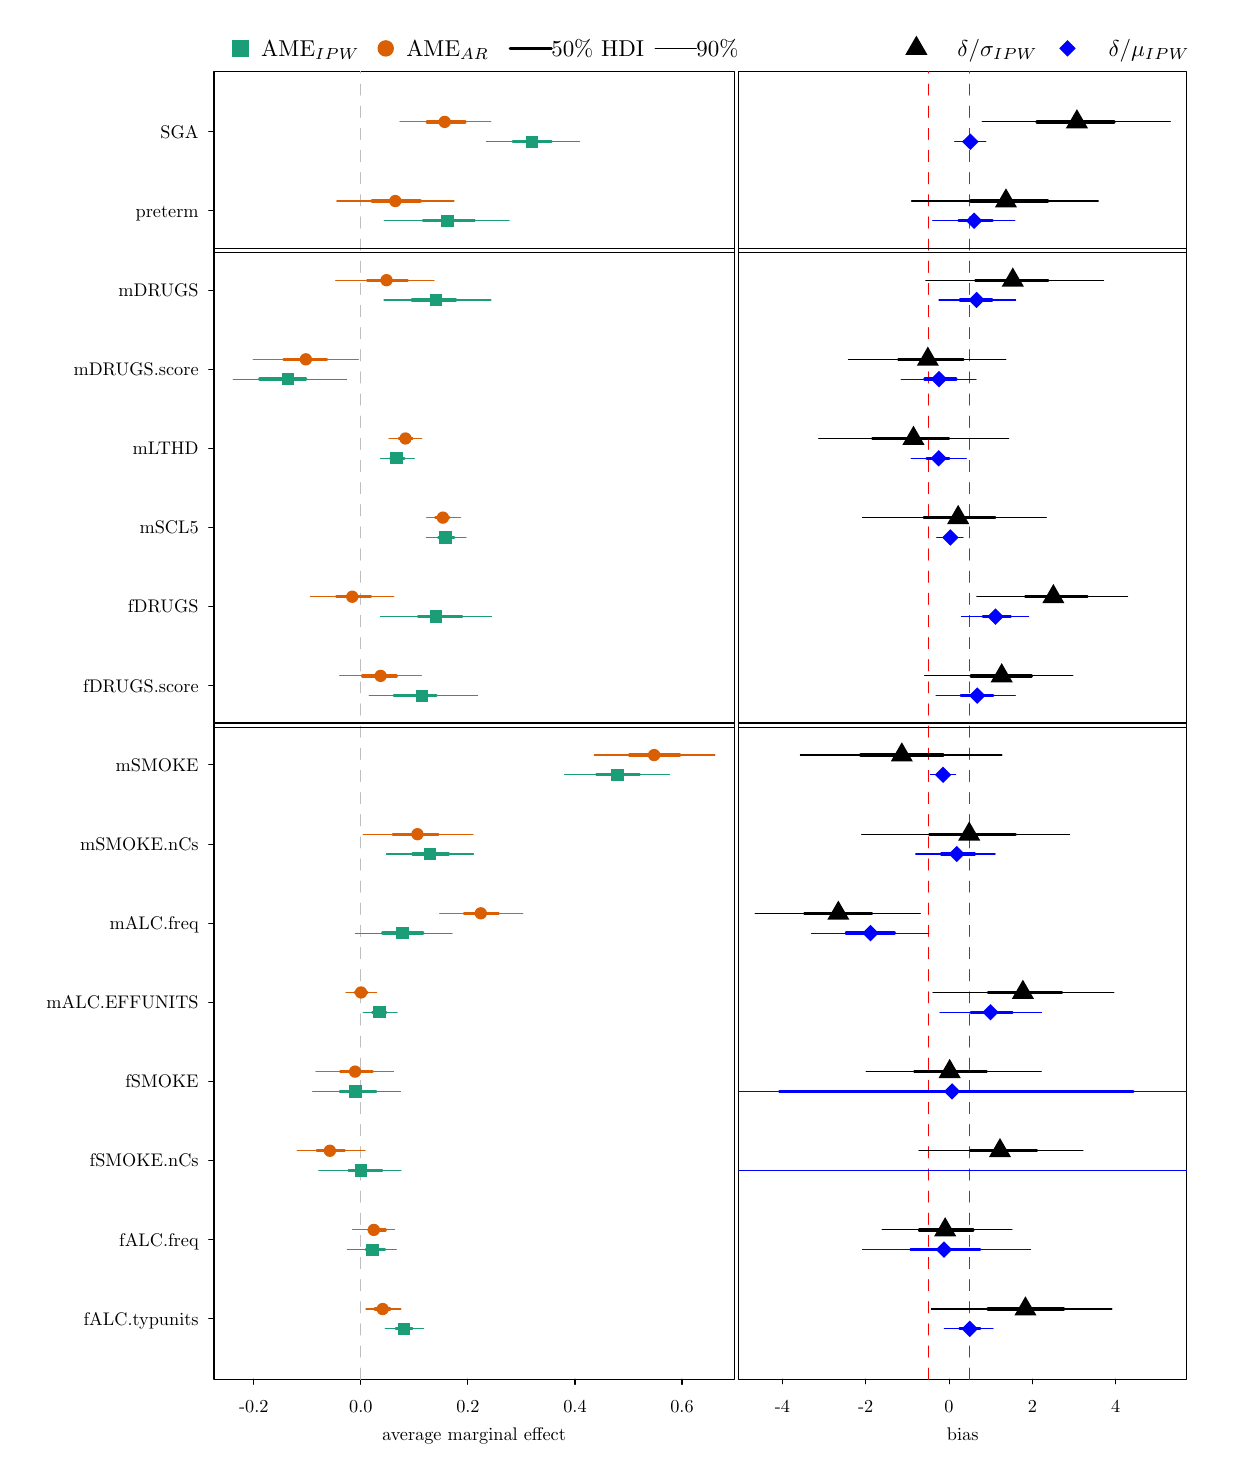
\begin{tikzpicture}[x=1pt,y=1pt]
\definecolor{fillColor}{RGB}{255,255,255}
\path[use as bounding box,fill=fillColor,fill opacity=0.00] (0,0) rectangle (426.79,512.15);
\begin{scope}
\path[clip] (  0.00,  0.00) rectangle (426.79,512.15);
\definecolor{drawColor}{RGB}{0,0,0}

\path[draw=drawColor,line width= 0.4pt,line join=round,line cap=round] ( 81.73, 23.76) -- (236.45, 23.76);

\path[draw=drawColor,line width= 0.4pt,line join=round,line cap=round] ( 81.73, 23.76) -- ( 81.73, 21.88);

\path[draw=drawColor,line width= 0.4pt,line join=round,line cap=round] (120.41, 23.76) -- (120.41, 21.88);

\path[draw=drawColor,line width= 0.4pt,line join=round,line cap=round] (159.09, 23.76) -- (159.09, 21.88);

\path[draw=drawColor,line width= 0.4pt,line join=round,line cap=round] (197.77, 23.76) -- (197.77, 21.88);

\path[draw=drawColor,line width= 0.4pt,line join=round,line cap=round] (236.45, 23.76) -- (236.45, 21.88);

\node[text=drawColor,anchor=base,inner sep=0pt, outer sep=0pt, scale=  0.66] at ( 81.73, 11.88) {-0.2};

\node[text=drawColor,anchor=base,inner sep=0pt, outer sep=0pt, scale=  0.66] at (120.41, 11.88) {0.0};

\node[text=drawColor,anchor=base,inner sep=0pt, outer sep=0pt, scale=  0.66] at (159.09, 11.88) {0.2};

\node[text=drawColor,anchor=base,inner sep=0pt, outer sep=0pt, scale=  0.66] at (197.77, 11.88) {0.4};

\node[text=drawColor,anchor=base,inner sep=0pt, outer sep=0pt, scale=  0.66] at (236.45, 11.88) {0.6};

\path[draw=drawColor,line width= 0.4pt,line join=round,line cap=round] ( 67.32, 23.76) --
	(255.28, 23.76) --
	(255.28,496.31) --
	( 67.32,496.31) --
	( 67.32, 23.76);
\end{scope}
\begin{scope}
\path[clip] (  0.00,  0.00) rectangle (256.07,512.15);
\definecolor{drawColor}{RGB}{0,0,0}

\node[text=drawColor,anchor=base,inner sep=0pt, outer sep=0pt, scale=  0.66] at (161.30,  1.58) {average marginal effect};
\end{scope}
\begin{scope}
\path[clip] ( 67.32, 23.76) rectangle (255.28,496.31);
\definecolor{drawColor}{RGB}{190,190,190}

\path[draw=drawColor,line width= 0.4pt,dash pattern=on 4pt off 4pt ,line join=round,line cap=round] (120.41, 23.76) -- (120.41,496.31);
\definecolor{fillColor}{RGB}{27,158,119}

\path[fill=fillColor] (180.11,468.72) --
	(184.57,468.72) --
	(184.57,473.17) --
	(180.11,473.17) --
	cycle;

\path[fill=fillColor] (149.45,440.12) --
	(153.90,440.12) --
	(153.90,444.57) --
	(149.45,444.57) --
	cycle;

\path[fill=fillColor] (145.38,411.52) --
	(149.84,411.52) --
	(149.84,415.98) --
	(145.38,415.98) --
	cycle;

\path[fill=fillColor] ( 91.94,382.92) --
	( 96.39,382.92) --
	( 96.39,387.38) --
	( 91.94,387.38) --
	cycle;

\path[fill=fillColor] (131.09,354.32) --
	(135.54,354.32) --
	(135.54,358.78) --
	(131.09,358.78) --
	cycle;

\path[fill=fillColor] (148.78,325.73) --
	(153.24,325.73) --
	(153.24,330.18) --
	(148.78,330.18) --
	cycle;

\path[fill=fillColor] (145.42,297.13) --
	(149.87,297.13) --
	(149.87,301.58) --
	(145.42,301.58) --
	cycle;

\path[fill=fillColor] (140.20,268.53) --
	(144.66,268.53) --
	(144.66,272.99) --
	(140.20,272.99) --
	cycle;

\path[fill=fillColor] (210.92,239.93) --
	(215.38,239.93) --
	(215.38,244.39) --
	(210.92,244.39) --
	cycle;

\path[fill=fillColor] (143.25,211.34) --
	(147.71,211.34) --
	(147.71,215.79) --
	(143.25,215.79) --
	cycle;

\path[fill=fillColor] (133.19,182.74) --
	(137.65,182.74) --
	(137.65,187.19) --
	(133.19,187.19) --
	cycle;

\path[fill=fillColor] (124.85,154.14) --
	(129.30,154.14) --
	(129.30,158.60) --
	(124.85,158.60) --
	cycle;

\path[fill=fillColor] (116.21,125.54) --
	(120.67,125.54) --
	(120.67,130.00) --
	(116.21,130.00) --
	cycle;

\path[fill=fillColor] (118.34, 96.94) --
	(122.79, 96.94) --
	(122.79,101.40) --
	(118.34,101.40) --
	cycle;

\path[fill=fillColor] (122.35, 68.35) --
	(126.80, 68.35) --
	(126.80, 72.80) --
	(122.35, 72.80) --
	cycle;

\path[fill=fillColor] (133.84, 39.75) --
	(138.29, 39.75) --
	(138.29, 44.20) --
	(133.84, 44.20) --
	cycle;
\definecolor{drawColor}{RGB}{27,158,119}

\path[draw=drawColor,line width= 1.2pt,line join=round,line cap=round] (175.33,470.94) -- (189.22,470.94);

\path[draw=drawColor,line width= 1.2pt,line join=round,line cap=round] (142.87,442.35) -- (161.46,442.35);

\path[draw=drawColor,line width= 1.2pt,line join=round,line cap=round] (138.95,413.75) -- (154.58,413.75);

\path[draw=drawColor,line width= 1.2pt,line join=round,line cap=round] ( 83.89,385.15) -- (100.40,385.15);

\path[draw=drawColor,line width= 1.2pt,line join=round,line cap=round] (131.05,356.55) -- (136.06,356.55);

\path[draw=drawColor,line width= 1.2pt,line join=round,line cap=round] (148.43,327.95) -- (154.09,327.95);

\path[draw=drawColor,line width= 1.2pt,line join=round,line cap=round] (141.09,299.36) -- (156.98,299.36);

\path[draw=drawColor,line width= 1.2pt,line join=round,line cap=round] (132.35,270.76) -- (147.68,270.76);

\path[draw=drawColor,line width= 1.2pt,line join=round,line cap=round] (205.51,242.16) -- (221.12,242.16);

\path[draw=drawColor,line width= 1.2pt,line join=round,line cap=round] (139.19,213.56) -- (152.00,213.56);

\path[draw=drawColor,line width= 1.2pt,line join=round,line cap=round] (128.30,184.97) -- (142.75,184.97);

\path[draw=drawColor,line width= 1.2pt,line join=round,line cap=round] (124.54,156.37) -- (129.55,156.37);

\path[draw=drawColor,line width= 1.2pt,line join=round,line cap=round] (112.85,127.77) -- (125.88,127.77);

\path[draw=drawColor,line width= 1.2pt,line join=round,line cap=round] (116.00, 99.17) -- (128.07, 99.17);

\path[draw=drawColor,line width= 1.2pt,line join=round,line cap=round] (122.24, 70.57) -- (129.02, 70.57);

\path[draw=drawColor,line width= 1.2pt,line join=round,line cap=round] (133.09, 41.98) -- (138.95, 41.98);

\path[draw=drawColor,line width= 0.4pt,line join=round,line cap=round] (165.78,470.94) -- (199.46,470.94);

\path[draw=drawColor,line width= 0.4pt,line join=round,line cap=round] (128.81,442.35) -- (173.96,442.35);

\path[draw=drawColor,line width= 0.4pt,line join=round,line cap=round] (128.76,413.75) -- (167.41,413.75);

\path[draw=drawColor,line width= 0.4pt,line join=round,line cap=round] ( 74.28,385.15) -- (115.23,385.15);

\path[draw=drawColor,line width= 0.4pt,line join=round,line cap=round] (127.47,356.55) -- (139.76,356.55);

\path[draw=drawColor,line width= 0.4pt,line join=round,line cap=round] (144.12,327.95) -- (158.43,327.95);

\path[draw=drawColor,line width= 0.4pt,line join=round,line cap=round] (127.46,299.36) -- (167.62,299.36);

\path[draw=drawColor,line width= 0.4pt,line join=round,line cap=round] (123.42,270.76) -- (162.54,270.76);

\path[draw=drawColor,line width= 0.4pt,line join=round,line cap=round] (193.96,242.16) -- (231.99,242.16);

\path[draw=drawColor,line width= 0.4pt,line join=round,line cap=round] (129.64,213.56) -- (161.10,213.56);

\path[draw=drawColor,line width= 0.4pt,line join=round,line cap=round] (118.46,184.97) -- (153.33,184.97);

\path[draw=drawColor,line width= 0.4pt,line join=round,line cap=round] (121.20,156.37) -- (133.47,156.37);

\path[draw=drawColor,line width= 0.4pt,line join=round,line cap=round] (102.98,127.77) -- (134.74,127.77);

\path[draw=drawColor,line width= 0.4pt,line join=round,line cap=round] (105.17, 99.17) -- (134.93, 99.17);

\path[draw=drawColor,line width= 0.4pt,line join=round,line cap=round] (115.51, 70.57) -- (133.20, 70.57);

\path[draw=drawColor,line width= 0.4pt,line join=round,line cap=round] (129.17, 41.98) -- (143.08, 41.98);
\definecolor{fillColor}{RGB}{217,95,2}

\path[fill=fillColor] (150.68,478.09) circle (  2.23);

\path[fill=fillColor] (132.85,449.50) circle (  2.23);

\path[fill=fillColor] (129.67,420.90) circle (  2.23);

\path[fill=fillColor] (100.52,392.30) circle (  2.23);

\path[fill=fillColor] (136.52,363.70) circle (  2.23);

\path[fill=fillColor] (150.05,335.10) circle (  2.23);

\path[fill=fillColor] (117.28,306.51) circle (  2.23);

\path[fill=fillColor] (127.53,277.91) circle (  2.23);

\path[fill=fillColor] (226.36,249.31) circle (  2.23);

\path[fill=fillColor] (140.85,220.71) circle (  2.23);

\path[fill=fillColor] (163.73,192.12) circle (  2.23);

\path[fill=fillColor] (120.45,163.52) circle (  2.23);

\path[fill=fillColor] (118.30,134.92) circle (  2.23);

\path[fill=fillColor] (109.20,106.32) circle (  2.23);

\path[fill=fillColor] (125.08, 77.72) circle (  2.23);

\path[fill=fillColor] (128.29, 49.13) circle (  2.23);
\definecolor{drawColor}{RGB}{217,95,2}

\path[draw=drawColor,line width= 1.2pt,line join=round,line cap=round] (144.42,478.09) -- (157.97,478.09);

\path[draw=drawColor,line width= 1.2pt,line join=round,line cap=round] (124.49,449.50) -- (141.84,449.50);

\path[draw=drawColor,line width= 1.2pt,line join=round,line cap=round] (122.73,420.90) -- (137.26,420.90);

\path[draw=drawColor,line width= 1.2pt,line join=round,line cap=round] ( 92.52,392.30) -- (108.08,392.30);

\path[draw=drawColor,line width= 1.2pt,line join=round,line cap=round] (134.16,363.70) -- (138.97,363.70);

\path[draw=drawColor,line width= 1.2pt,line join=round,line cap=round] (147.35,335.10) -- (152.31,335.10);

\path[draw=drawColor,line width= 1.2pt,line join=round,line cap=round] (111.54,306.51) -- (124.03,306.51);

\path[draw=drawColor,line width= 1.2pt,line join=round,line cap=round] (121.04,277.91) -- (133.17,277.91);

\path[draw=drawColor,line width= 1.2pt,line join=round,line cap=round] (217.51,249.31) -- (235.54,249.31);

\path[draw=drawColor,line width= 1.2pt,line join=round,line cap=round] (131.96,220.71) -- (148.38,220.71);

\path[draw=drawColor,line width= 1.2pt,line join=round,line cap=round] (157.74,192.12) -- (170.18,192.12);

\path[draw=drawColor,line width= 1.2pt,line join=round,line cap=round] (118.21,163.52) -- (122.75,163.52);

\path[draw=drawColor,line width= 1.2pt,line join=round,line cap=round] (112.98,134.92) -- (124.62,134.92);

\path[draw=drawColor,line width= 1.2pt,line join=round,line cap=round] (104.50,106.32) -- (114.48,106.32);

\path[draw=drawColor,line width= 1.2pt,line join=round,line cap=round] (123.36, 77.72) -- (129.17, 77.72);

\path[draw=drawColor,line width= 1.2pt,line join=round,line cap=round] (125.57, 49.13) -- (130.80, 49.13);

\path[draw=drawColor,line width= 0.4pt,line join=round,line cap=round] (134.51,478.09) -- (167.37,478.09);

\path[draw=drawColor,line width= 0.4pt,line join=round,line cap=round] (111.72,449.50) -- (154.06,449.50);

\path[draw=drawColor,line width= 0.4pt,line join=round,line cap=round] (111.26,420.90) -- (146.87,420.90);

\path[draw=drawColor,line width= 0.4pt,line join=round,line cap=round] ( 81.47,392.30) -- (119.49,392.30);

\path[draw=drawColor,line width= 0.4pt,line join=round,line cap=round] (130.57,363.70) -- (142.38,363.70);

\path[draw=drawColor,line width= 0.4pt,line join=round,line cap=round] (144.16,335.10) -- (156.44,335.10);

\path[draw=drawColor,line width= 0.4pt,line join=round,line cap=round] (102.16,306.51) -- (132.30,306.51);

\path[draw=drawColor,line width= 0.4pt,line join=round,line cap=round] (112.72,277.91) -- (142.22,277.91);

\path[draw=drawColor,line width= 0.4pt,line join=round,line cap=round] (204.77,249.31) -- (248.32,249.31);

\path[draw=drawColor,line width= 0.4pt,line join=round,line cap=round] (121.26,220.71) -- (160.95,220.71);

\path[draw=drawColor,line width= 0.4pt,line join=round,line cap=round] (148.87,192.12) -- (178.91,192.12);

\path[draw=drawColor,line width= 0.4pt,line join=round,line cap=round] (114.98,163.52) -- (126.07,163.52);

\path[draw=drawColor,line width= 0.4pt,line join=round,line cap=round] (104.12,134.92) -- (132.21,134.92);

\path[draw=drawColor,line width= 0.4pt,line join=round,line cap=round] ( 97.41,106.32) -- (121.89,106.32);

\path[draw=drawColor,line width= 0.4pt,line join=round,line cap=round] (117.36, 77.72) -- (132.56, 77.72);

\path[draw=drawColor,line width= 0.4pt,line join=round,line cap=round] (122.25, 49.13) -- (134.87, 49.13);
\end{scope}
\begin{scope}
\path[clip] (  0.00,  0.00) rectangle (426.79,512.15);
\definecolor{drawColor}{RGB}{0,0,0}

\path[draw=drawColor,line width= 0.4pt,line join=round,line cap=round] ( 67.32, 45.55) -- ( 67.32,474.52);

\path[draw=drawColor,line width= 0.4pt,line join=round,line cap=round] ( 67.32, 45.55) -- ( 65.44, 45.55);

\path[draw=drawColor,line width= 0.4pt,line join=round,line cap=round] ( 67.32, 74.15) -- ( 65.44, 74.15);

\path[draw=drawColor,line width= 0.4pt,line join=round,line cap=round] ( 67.32,102.75) -- ( 65.44,102.75);

\path[draw=drawColor,line width= 0.4pt,line join=round,line cap=round] ( 67.32,131.34) -- ( 65.44,131.34);

\path[draw=drawColor,line width= 0.4pt,line join=round,line cap=round] ( 67.32,159.94) -- ( 65.44,159.94);

\path[draw=drawColor,line width= 0.4pt,line join=round,line cap=round] ( 67.32,188.54) -- ( 65.44,188.54);

\path[draw=drawColor,line width= 0.4pt,line join=round,line cap=round] ( 67.32,217.14) -- ( 65.44,217.14);

\path[draw=drawColor,line width= 0.4pt,line join=round,line cap=round] ( 67.32,245.74) -- ( 65.44,245.74);

\path[draw=drawColor,line width= 0.4pt,line join=round,line cap=round] ( 67.32,274.33) -- ( 65.44,274.33);

\path[draw=drawColor,line width= 0.4pt,line join=round,line cap=round] ( 67.32,302.93) -- ( 65.44,302.93);

\path[draw=drawColor,line width= 0.4pt,line join=round,line cap=round] ( 67.32,331.53) -- ( 65.44,331.53);

\path[draw=drawColor,line width= 0.4pt,line join=round,line cap=round] ( 67.32,360.13) -- ( 65.44,360.13);

\path[draw=drawColor,line width= 0.4pt,line join=round,line cap=round] ( 67.32,388.72) -- ( 65.44,388.72);

\path[draw=drawColor,line width= 0.4pt,line join=round,line cap=round] ( 67.32,417.32) -- ( 65.44,417.32);

\path[draw=drawColor,line width= 0.4pt,line join=round,line cap=round] ( 67.32,445.92) -- ( 65.44,445.92);

\path[draw=drawColor,line width= 0.4pt,line join=round,line cap=round] ( 67.32,474.52) -- ( 65.44,474.52);

\node[text=drawColor,anchor=base east,inner sep=0pt, outer sep=0pt, scale=  0.66] at ( 61.78, 43.28) {fALC.typunits};

\node[text=drawColor,anchor=base east,inner sep=0pt, outer sep=0pt, scale=  0.66] at ( 61.78, 71.88) {fALC.freq};

\node[text=drawColor,anchor=base east,inner sep=0pt, outer sep=0pt, scale=  0.66] at ( 61.78,100.47) {fSMOKE.nCs};

\node[text=drawColor,anchor=base east,inner sep=0pt, outer sep=0pt, scale=  0.66] at ( 61.78,129.07) {fSMOKE};

\node[text=drawColor,anchor=base east,inner sep=0pt, outer sep=0pt, scale=  0.66] at ( 61.78,157.67) {mALC.EFFUNITS};

\node[text=drawColor,anchor=base east,inner sep=0pt, outer sep=0pt, scale=  0.66] at ( 61.78,186.27) {mALC.freq};

\node[text=drawColor,anchor=base east,inner sep=0pt, outer sep=0pt, scale=  0.66] at ( 61.78,214.87) {mSMOKE.nCs};

\node[text=drawColor,anchor=base east,inner sep=0pt, outer sep=0pt, scale=  0.66] at ( 61.78,243.46) {mSMOKE};

\node[text=drawColor,anchor=base east,inner sep=0pt, outer sep=0pt, scale=  0.66] at ( 61.78,272.06) {fDRUGS.score};

\node[text=drawColor,anchor=base east,inner sep=0pt, outer sep=0pt, scale=  0.66] at ( 61.78,300.66) {fDRUGS};

\node[text=drawColor,anchor=base east,inner sep=0pt, outer sep=0pt, scale=  0.66] at ( 61.78,329.26) {mSCL5};

\node[text=drawColor,anchor=base east,inner sep=0pt, outer sep=0pt, scale=  0.66] at ( 61.78,357.85) {mLTHD};

\node[text=drawColor,anchor=base east,inner sep=0pt, outer sep=0pt, scale=  0.66] at ( 61.78,386.45) {mDRUGS.score};

\node[text=drawColor,anchor=base east,inner sep=0pt, outer sep=0pt, scale=  0.66] at ( 61.78,415.05) {mDRUGS};

\node[text=drawColor,anchor=base east,inner sep=0pt, outer sep=0pt, scale=  0.66] at ( 61.78,443.65) {preterm};

\node[text=drawColor,anchor=base east,inner sep=0pt, outer sep=0pt, scale=  0.66] at ( 61.78,472.25) {SGA};
\end{scope}
\begin{scope}
\path[clip] (  0.00,  0.00) rectangle (256.07,512.15);

\path[] ( 69.55,504.65) -- ( 84.40,504.65);

\path[] (121.95,504.65) -- (136.80,504.65);
\definecolor{drawColor}{RGB}{0,0,0}

\path[draw=drawColor,line width= 1.2pt,line join=round,line cap=round] (174.35,504.65) -- (189.20,504.65);

\path[draw=drawColor,line width= 0.4pt,line join=round,line cap=round] (226.76,504.65) -- (241.61,504.65);
\definecolor{fillColor}{RGB}{27,158,119}

\path[fill=fillColor] ( 74.00,501.68) --
	( 79.94,501.68) --
	( 79.94,507.62) --
	( 74.00,507.62) --
	cycle;
\definecolor{fillColor}{RGB}{217,95,2}

\path[fill=fillColor] (129.38,504.65) circle (  2.97);

\node[text=drawColor,anchor=base west,inner sep=0pt, outer sep=0pt, scale=  0.83] at ( 84.40,501.81) {AME$_{IPW}$};

\node[text=drawColor,anchor=base west,inner sep=0pt, outer sep=0pt, scale=  0.83] at (136.80,501.81) {AME$_{AR}$};

\node[text=drawColor,anchor=base west,inner sep=0pt, outer sep=0pt, scale=  0.83] at (189.20,501.81) {50\% HDI};

\node[text=drawColor,anchor=base west,inner sep=0pt, outer sep=0pt, scale=  0.83] at (241.61,501.81) {90\% HDI};
\end{scope}
\begin{scope}
\path[clip] ( 67.32, 23.76) rectangle (255.28,496.31);
\definecolor{drawColor}{RGB}{0,0,0}

\path[draw=drawColor,line width= 0.4pt,line join=round,line cap=round] ( 67.32,430.76) -- (255.28,430.76);

\path[draw=drawColor,line width= 0.4pt,line join=round,line cap=round] ( 67.32,432.48) -- (255.28,432.48);

\path[draw=drawColor,line width= 0.4pt,line join=round,line cap=round] ( 67.32,259.18) -- (255.28,259.18);

\path[draw=drawColor,line width= 0.4pt,line join=round,line cap=round] ( 67.32,260.89) -- (255.28,260.89);
\end{scope}
\begin{scope}
\path[clip] (  0.00,  0.00) rectangle (426.79,512.15);
\definecolor{drawColor}{RGB}{0,0,0}

\path[draw=drawColor,line width= 0.4pt,line join=round,line cap=round] (272.72, 23.76) -- (393.15, 23.76);

\path[draw=drawColor,line width= 0.4pt,line join=round,line cap=round] (272.72, 23.76) -- (272.72, 22.14);

\path[draw=drawColor,line width= 0.4pt,line join=round,line cap=round] (302.83, 23.76) -- (302.83, 22.14);

\path[draw=drawColor,line width= 0.4pt,line join=round,line cap=round] (332.94, 23.76) -- (332.94, 22.14);

\path[draw=drawColor,line width= 0.4pt,line join=round,line cap=round] (363.05, 23.76) -- (363.05, 22.14);

\path[draw=drawColor,line width= 0.4pt,line join=round,line cap=round] (393.15, 23.76) -- (393.15, 22.14);

\node[text=drawColor,anchor=base,inner sep=0pt, outer sep=0pt, scale=  0.66] at (272.72, 11.88) {-4};

\node[text=drawColor,anchor=base,inner sep=0pt, outer sep=0pt, scale=  0.66] at (302.83, 11.88) {-2};

\node[text=drawColor,anchor=base,inner sep=0pt, outer sep=0pt, scale=  0.66] at (332.94, 11.88) {0};

\node[text=drawColor,anchor=base,inner sep=0pt, outer sep=0pt, scale=  0.66] at (363.05, 11.88) {2};

\node[text=drawColor,anchor=base,inner sep=0pt, outer sep=0pt, scale=  0.66] at (393.15, 11.88) {4};

\path[draw=drawColor,line width= 0.4pt,line join=round,line cap=round] (256.87, 23.76) --
	(418.87, 23.76) --
	(418.87,496.31) --
	(256.87,496.31) --
	(256.87, 23.76);
\end{scope}
\begin{scope}
\path[clip] (256.07,  0.00) rectangle (426.79,512.15);
\definecolor{drawColor}{RGB}{0,0,0}

\node[text=drawColor,anchor=base,inner sep=0pt, outer sep=0pt, scale=  0.66] at (337.87,  1.58) {bias};
\end{scope}
\begin{scope}
\path[clip] (256.87, 23.76) rectangle (418.87,496.31);
\definecolor{drawColor}{RGB}{255,0,0}

\path[draw=drawColor,line width= 0.4pt,dash pattern=on 4pt off 4pt ,line join=round,line cap=round] (325.41, 23.76) -- (325.41,496.31);

\path[draw=drawColor,line width= 0.4pt,dash pattern=on 4pt off 4pt ,line join=round,line cap=round] (340.47, 23.76) -- (340.47,496.31);
\definecolor{drawColor}{RGB}{0,0,0}

\path[draw=drawColor,line width= 0.4pt,line join=round,line cap=round] (344.92,478.09) -- (412.87,478.09);

\path[draw=drawColor,line width= 0.4pt,line join=round,line cap=round] (319.39,449.50) -- (386.85,449.50);

\path[draw=drawColor,line width= 0.4pt,line join=round,line cap=round] (324.53,420.90) -- (388.76,420.90);

\path[draw=drawColor,line width= 0.4pt,line join=round,line cap=round] (296.54,392.30) -- (353.45,392.30);

\path[draw=drawColor,line width= 0.4pt,line join=round,line cap=round] (285.78,363.70) -- (354.49,363.70);

\path[draw=drawColor,line width= 0.4pt,line join=round,line cap=round] (301.63,335.10) -- (368.09,335.10);

\path[draw=drawColor,line width= 0.4pt,line join=round,line cap=round] (342.96,306.51) -- (397.47,306.51);

\path[draw=drawColor,line width= 0.4pt,line join=round,line cap=round] (324.16,277.91) -- (377.63,277.91);

\path[draw=drawColor,line width= 0.4pt,line join=round,line cap=round] (279.20,249.31) -- (352.04,249.31);

\path[draw=drawColor,line width= 0.4pt,line join=round,line cap=round] (301.38,220.71) -- (376.52,220.71);

\path[draw=drawColor,line width= 0.4pt,line join=round,line cap=round] (262.87,192.12) -- (322.58,192.12);

\path[draw=drawColor,line width= 0.4pt,line join=round,line cap=round] (327.08,163.52) -- (392.47,163.52);

\path[draw=drawColor,line width= 0.4pt,line join=round,line cap=round] (303.00,134.92) -- (366.24,134.92);

\path[draw=drawColor,line width= 0.4pt,line join=round,line cap=round] (322.05,106.32) -- (381.32,106.32);

\path[draw=drawColor,line width= 0.4pt,line join=round,line cap=round] (308.74, 77.72) -- (355.67, 77.72);

\path[draw=drawColor,line width= 0.4pt,line join=round,line cap=round] (326.55, 49.13) -- (391.78, 49.13);

\path[draw=drawColor,line width= 1.2pt,line join=round,line cap=round] (364.77,478.09) -- (392.50,478.09);

\path[draw=drawColor,line width= 1.2pt,line join=round,line cap=round] (340.80,449.50) -- (368.51,449.50);

\path[draw=drawColor,line width= 1.2pt,line join=round,line cap=round] (342.45,420.90) -- (368.72,420.90);

\path[draw=drawColor,line width= 1.2pt,line join=round,line cap=round] (314.62,392.30) -- (338.08,392.30);

\path[draw=drawColor,line width= 1.2pt,line join=round,line cap=round] (305.25,363.70) -- (332.89,363.70);

\path[draw=drawColor,line width= 1.2pt,line join=round,line cap=round] (323.86,335.10) -- (349.56,335.10);

\path[draw=drawColor,line width= 1.2pt,line join=round,line cap=round] (360.50,306.51) -- (382.92,306.51);

\path[draw=drawColor,line width= 1.2pt,line join=round,line cap=round] (340.98,277.91) -- (362.62,277.91);

\path[draw=drawColor,line width= 1.2pt,line join=round,line cap=round] (301.02,249.31) -- (330.72,249.31);

\path[draw=drawColor,line width= 1.2pt,line join=round,line cap=round] (325.88,220.71) -- (356.93,220.71);

\path[draw=drawColor,line width= 1.2pt,line join=round,line cap=round] (280.68,192.12) -- (305.02,192.12);

\path[draw=drawColor,line width= 1.2pt,line join=round,line cap=round] (347.04,163.52) -- (373.65,163.52);

\path[draw=drawColor,line width= 1.2pt,line join=round,line cap=round] (320.45,134.92) -- (346.49,134.92);

\path[draw=drawColor,line width= 1.2pt,line join=round,line cap=round] (340.67,106.32) -- (364.64,106.32);

\path[draw=drawColor,line width= 1.2pt,line join=round,line cap=round] (322.25, 77.72) -- (341.55, 77.72);

\path[draw=drawColor,line width= 1.2pt,line join=round,line cap=round] (347.07, 49.13) -- (374.29, 49.13);
\definecolor{drawColor}{RGB}{0,0,255}

\path[draw=drawColor,line width= 0.4pt,line join=round,line cap=round] (334.93,470.94) -- (346.26,470.94);

\path[draw=drawColor,line width= 0.4pt,line join=round,line cap=round] (326.97,442.35) -- (356.70,442.35);

\path[draw=drawColor,line width= 0.4pt,line join=round,line cap=round] (329.31,413.75) -- (357.01,413.75);

\path[draw=drawColor,line width= 0.4pt,line join=round,line cap=round] (315.63,385.15) -- (342.69,385.15);

\path[draw=drawColor,line width= 0.4pt,line join=round,line cap=round] (319.23,356.55) -- (339.20,356.55);

\path[draw=drawColor,line width= 0.4pt,line join=round,line cap=round] (328.42,327.95) -- (338.01,327.95);

\path[draw=drawColor,line width= 0.4pt,line join=round,line cap=round] (337.40,299.36) -- (361.67,299.36);

\path[draw=drawColor,line width= 0.4pt,line join=round,line cap=round] (328.23,270.76) -- (356.87,270.76);

\path[draw=drawColor,line width= 0.4pt,line join=round,line cap=round] (326.19,242.16) -- (335.34,242.16);

\path[draw=drawColor,line width= 0.4pt,line join=round,line cap=round] (320.89,213.56) -- (349.58,213.56);

\path[draw=drawColor,line width= 0.4pt,line join=round,line cap=round] (283.21,184.97) -- (325.59,184.97);

\path[draw=drawColor,line width= 0.4pt,line join=round,line cap=round] (329.65,156.37) -- (366.36,156.37);

\path[draw=drawColor,line width= 0.4pt,line join=round,line cap=round] (185.92,127.77) -- (426.79,127.77);

\path[draw=drawColor,line width= 0.4pt,line join=round,line cap=round] (  0.00, 99.17) -- (426.79, 99.17);

\path[draw=drawColor,line width= 0.4pt,line join=round,line cap=round] (301.59, 70.57) -- (362.39, 70.57);

\path[draw=drawColor,line width= 0.4pt,line join=round,line cap=round] (331.21, 41.98) -- (348.87, 41.98);

\path[draw=drawColor,line width= 1.2pt,line join=round,line cap=round] (338.24,470.94) -- (342.86,470.94);

\path[draw=drawColor,line width= 1.2pt,line join=round,line cap=round] (336.40,442.35) -- (348.62,442.35);

\path[draw=drawColor,line width= 1.2pt,line join=round,line cap=round] (337.04,413.75) -- (348.37,413.75);

\path[draw=drawColor,line width= 1.2pt,line join=round,line cap=round] (324.23,385.15) -- (335.38,385.15);

\path[draw=drawColor,line width= 1.2pt,line join=round,line cap=round] (324.89,356.55) -- (332.92,356.55);

\path[draw=drawColor,line width= 1.2pt,line join=round,line cap=round] (331.63,327.95) -- (335.34,327.95);

\path[draw=drawColor,line width= 1.2pt,line join=round,line cap=round] (345.21,299.36) -- (355.19,299.36);

\path[draw=drawColor,line width= 1.2pt,line join=round,line cap=round] (337.25,270.76) -- (348.83,270.76);

\path[draw=drawColor,line width= 1.2pt,line join=round,line cap=round] (328.93,242.16) -- (332.66,242.16);

\path[draw=drawColor,line width= 1.2pt,line join=round,line cap=round] (330.24,213.56) -- (342.10,213.56);

\path[draw=drawColor,line width= 1.2pt,line join=round,line cap=round] (295.85,184.97) -- (313.13,184.97);

\path[draw=drawColor,line width= 1.2pt,line join=round,line cap=round] (340.85,156.37) -- (355.79,156.37);

\path[draw=drawColor,line width= 1.2pt,line join=round,line cap=round] (271.62,127.77) -- (399.48,127.77);

\path[draw=drawColor,line width= 1.2pt,line join=round,line cap=round] (319.10, 70.57) -- (344.10, 70.57);

\path[draw=drawColor,line width= 1.2pt,line join=round,line cap=round] (336.77, 41.98) -- (344.13, 41.98);
\definecolor{fillColor}{RGB}{0,0,0}

\path[fill=fillColor] (379.14,482.71) --
	(383.14,475.78) --
	(375.14,475.78) --
	cycle;

\path[fill=fillColor] (353.50,454.11) --
	(357.50,447.19) --
	(349.50,447.19) --
	cycle;

\path[fill=fillColor] (355.97,425.52) --
	(359.97,418.59) --
	(351.97,418.59) --
	cycle;

\path[fill=fillColor] (325.28,396.92) --
	(329.27,389.99) --
	(321.28,389.99) --
	cycle;

\path[fill=fillColor] (320.08,368.32) --
	(324.08,361.39) --
	(316.08,361.39) --
	cycle;

\path[fill=fillColor] (336.23,339.72) --
	(340.23,332.79) --
	(332.23,332.79) --
	cycle;

\path[fill=fillColor] (370.63,311.12) --
	(374.63,304.20) --
	(366.63,304.20) --
	cycle;

\path[fill=fillColor] (351.96,282.53) --
	(355.96,275.60) --
	(347.96,275.60) --
	cycle;

\path[fill=fillColor] (315.87,253.93) --
	(319.87,247.00) --
	(311.87,247.00) --
	cycle;

\path[fill=fillColor] (340.22,225.33) --
	(344.22,218.40) --
	(336.22,218.40) --
	cycle;

\path[fill=fillColor] (292.93,196.73) --
	(296.93,189.81) --
	(288.93,189.81) --
	cycle;

\path[fill=fillColor] (359.62,168.14) --
	(363.62,161.21) --
	(355.62,161.21) --
	cycle;

\path[fill=fillColor] (333.16,139.54) --
	(337.16,132.61) --
	(329.16,132.61) --
	cycle;

\path[fill=fillColor] (351.34,110.94) --
	(355.34,104.01) --
	(347.34,104.01) --
	cycle;

\path[fill=fillColor] (331.53, 82.34) --
	(335.53, 75.41) --
	(327.53, 75.41) --
	cycle;

\path[fill=fillColor] (360.54, 53.74) --
	(364.54, 46.82) --
	(356.54, 46.82) --
	cycle;
\definecolor{fillColor}{RGB}{0,0,255}

\path[fill=fillColor] (337.67,470.94) --
	(340.64,473.91) --
	(343.61,470.94) --
	(340.64,467.97) --
	cycle;

\path[fill=fillColor] (339.03,442.35) --
	(342.00,445.32) --
	(344.97,442.35) --
	(342.00,439.38) --
	cycle;

\path[fill=fillColor] (339.90,413.75) --
	(342.87,416.72) --
	(345.84,413.75) --
	(342.87,410.78) --
	cycle;

\path[fill=fillColor] (326.32,385.15) --
	(329.29,388.12) --
	(332.26,385.15) --
	(329.29,382.18) --
	cycle;

\path[fill=fillColor] (326.23,356.55) --
	(329.20,359.52) --
	(332.17,356.55) --
	(329.20,353.58) --
	cycle;

\path[fill=fillColor] (330.44,327.95) --
	(333.41,330.92) --
	(336.38,327.95) --
	(333.41,324.98) --
	cycle;

\path[fill=fillColor] (346.75,299.36) --
	(349.72,302.33) --
	(352.69,299.36) --
	(349.72,296.39) --
	cycle;

\path[fill=fillColor] (340.16,270.76) --
	(343.13,273.73) --
	(346.10,270.76) --
	(343.13,267.79) --
	cycle;

\path[fill=fillColor] (327.82,242.16) --
	(330.79,245.13) --
	(333.76,242.16) --
	(330.79,239.19) --
	cycle;

\path[fill=fillColor] (332.75,213.56) --
	(335.72,216.53) --
	(338.69,213.56) --
	(335.72,210.59) --
	cycle;

\path[fill=fillColor] (301.57,184.97) --
	(304.54,187.94) --
	(307.51,184.97) --
	(304.54,182.00) --
	cycle;

\path[fill=fillColor] (344.94,156.37) --
	(347.91,159.34) --
	(350.88,156.37) --
	(347.91,153.40) --
	cycle;

\path[fill=fillColor] (331.06,127.77) --
	(334.03,130.74) --
	(337.00,127.77) --
	(334.03,124.80) --
	cycle;

\path[fill=fillColor] (328.14, 70.57) --
	(331.11, 73.54) --
	(334.08, 70.57) --
	(331.11, 67.60) --
	cycle;

\path[fill=fillColor] (337.44, 41.98) --
	(340.41, 44.95) --
	(343.38, 41.98) --
	(340.41, 39.01) --
	cycle;
\end{scope}
\begin{scope}
\path[clip] (256.07,  0.00) rectangle (426.79,512.15);
\definecolor{fillColor}{RGB}{0,0,0}

\path[fill=fillColor] (321.13,509.27) --
	(325.13,502.35) --
	(317.13,502.35) --
	cycle;
\definecolor{fillColor}{RGB}{0,0,255}

\path[fill=fillColor] (372.77,504.65) --
	(375.74,507.62) --
	(378.71,504.65) --
	(375.74,501.68) --
	cycle;
\definecolor{drawColor}{RGB}{0,0,0}

\node[text=drawColor,anchor=base west,inner sep=0pt, outer sep=0pt, scale=  0.83] at (281.37,501.81) { };

\node[text=drawColor,anchor=base west,inner sep=0pt, outer sep=0pt, scale=  0.83] at (335.98,501.81) {$\delta/\sigma_{IPW}$};

\node[text=drawColor,anchor=base west,inner sep=0pt, outer sep=0pt, scale=  0.83] at (390.59,501.81) {$\delta/\mu_{IPW}$};
\end{scope}
\begin{scope}
\path[clip] (256.87, 23.76) rectangle (418.87,496.31);
\definecolor{drawColor}{RGB}{0,0,0}

\path[draw=drawColor,line width= 0.4pt,line join=round,line cap=round] (256.87,430.76) -- (418.87,430.76);

\path[draw=drawColor,line width= 0.4pt,line join=round,line cap=round] (256.87,432.48) -- (418.87,432.48);

\path[draw=drawColor,line width= 0.4pt,line join=round,line cap=round] (256.87,259.18) -- (418.87,259.18);

\path[draw=drawColor,line width= 0.4pt,line join=round,line cap=round] (256.87,260.89) -- (418.87,260.89);
\end{scope}
\end{tikzpicture}
}
	\caption{Exposure-outcome association estimates. $AME_{AR}$: Average marginal effects from regression adjusted for participation predictors. $AME_{IPPW}$: $AME$ from inverse probability of participation weighted regression. $AME$s are for a one point increase of the exposure (all exposures except parity were standardized). HDI: Highest density interval of the posterior distribution. The right panel shows differences between the AR and IPPW estimates ($\delta = AME_{IPPW}-AME_{AR}$), standardized by the mean ($\mu_{IPPW}$) or the standard deviation ($\sigma_{IPPW}$) of the IPPW estimates. To confirm the absence of bias, the 90\% HDI should fall within a region of negligible differences between the AR and IPPW estimates. The two red lines enclose a region where the deviation is smaller than 50\% of the mean or standard deviation of the IPPW estimate.}
	\label{fig:estimates}
\end{figure}


\begin{table}
	\ifthenelse{\boolean{ismanus}}{}{% Created by tikzDevice version 0.11 on 2018-05-04 09:33:42
% !TEX encoding = UTF-8 Unicode
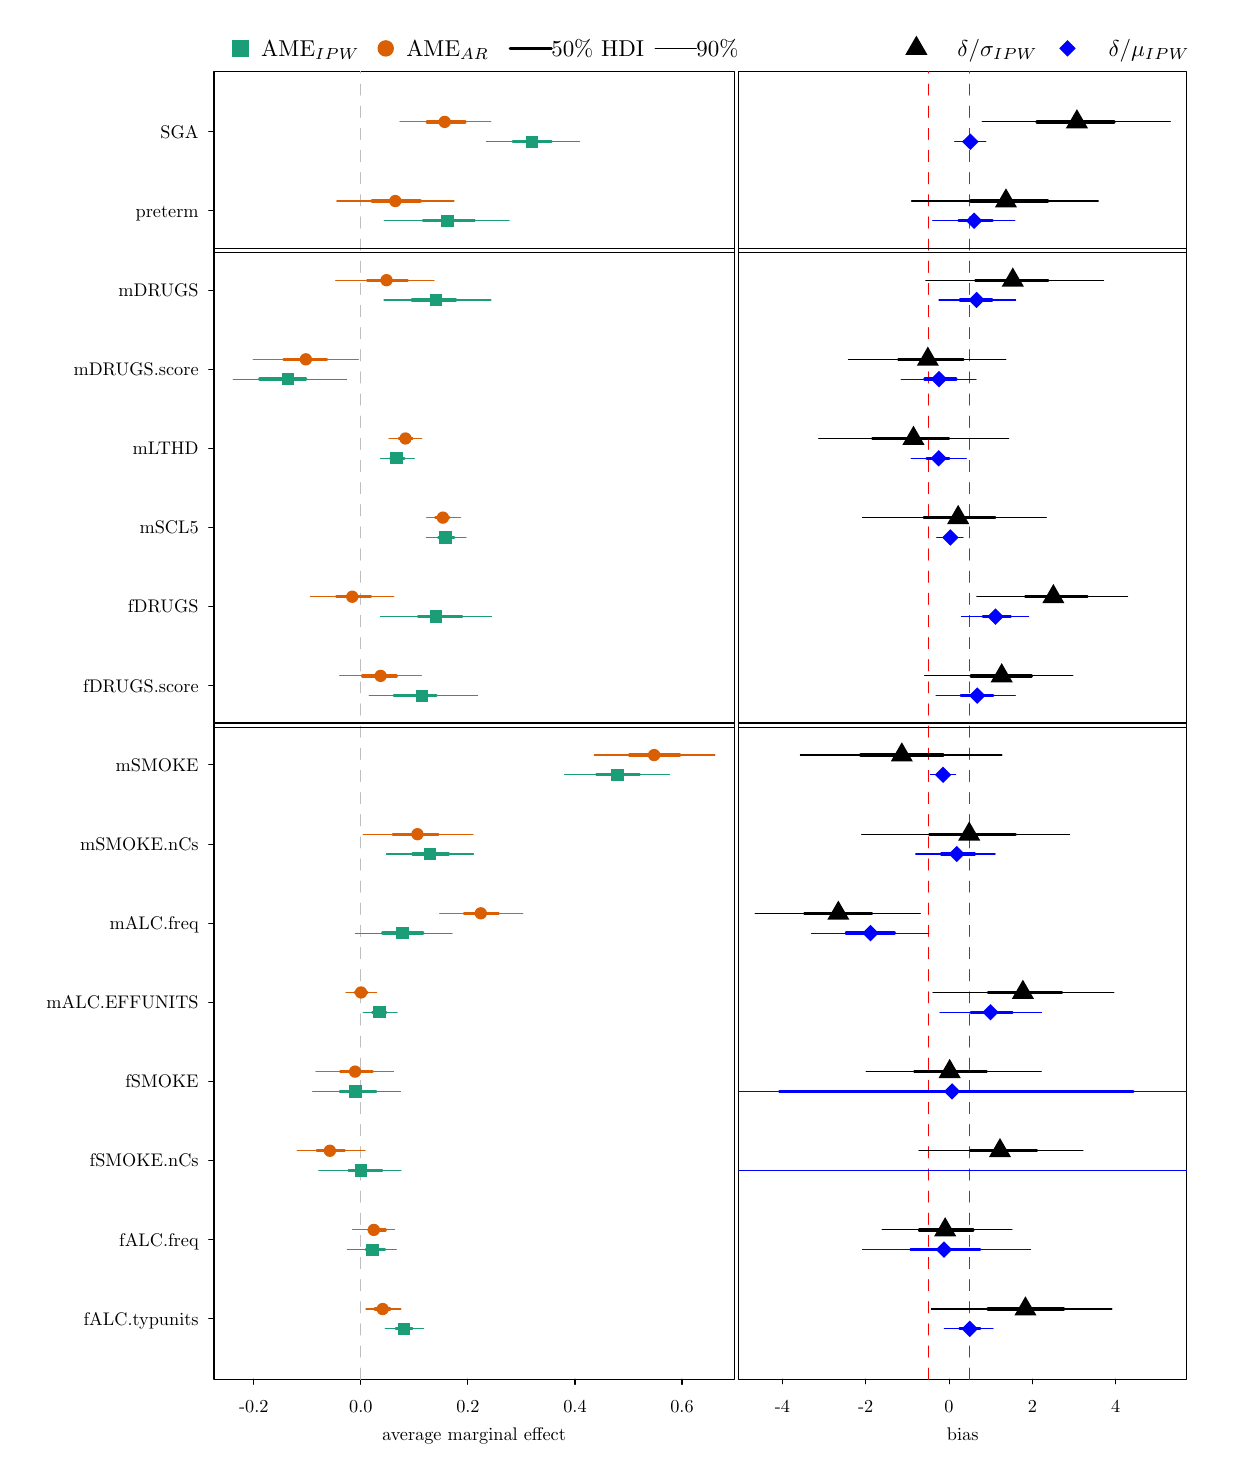
\begin{tikzpicture}[x=1pt,y=1pt]
\definecolor{fillColor}{RGB}{255,255,255}
\path[use as bounding box,fill=fillColor,fill opacity=0.00] (0,0) rectangle (426.79,512.15);
\begin{scope}
\path[clip] (  0.00,  0.00) rectangle (426.79,512.15);
\definecolor{drawColor}{RGB}{0,0,0}

\path[draw=drawColor,line width= 0.4pt,line join=round,line cap=round] ( 81.73, 23.76) -- (236.45, 23.76);

\path[draw=drawColor,line width= 0.4pt,line join=round,line cap=round] ( 81.73, 23.76) -- ( 81.73, 21.88);

\path[draw=drawColor,line width= 0.4pt,line join=round,line cap=round] (120.41, 23.76) -- (120.41, 21.88);

\path[draw=drawColor,line width= 0.4pt,line join=round,line cap=round] (159.09, 23.76) -- (159.09, 21.88);

\path[draw=drawColor,line width= 0.4pt,line join=round,line cap=round] (197.77, 23.76) -- (197.77, 21.88);

\path[draw=drawColor,line width= 0.4pt,line join=round,line cap=round] (236.45, 23.76) -- (236.45, 21.88);

\node[text=drawColor,anchor=base,inner sep=0pt, outer sep=0pt, scale=  0.66] at ( 81.73, 11.88) {-0.2};

\node[text=drawColor,anchor=base,inner sep=0pt, outer sep=0pt, scale=  0.66] at (120.41, 11.88) {0.0};

\node[text=drawColor,anchor=base,inner sep=0pt, outer sep=0pt, scale=  0.66] at (159.09, 11.88) {0.2};

\node[text=drawColor,anchor=base,inner sep=0pt, outer sep=0pt, scale=  0.66] at (197.77, 11.88) {0.4};

\node[text=drawColor,anchor=base,inner sep=0pt, outer sep=0pt, scale=  0.66] at (236.45, 11.88) {0.6};

\path[draw=drawColor,line width= 0.4pt,line join=round,line cap=round] ( 67.32, 23.76) --
	(255.28, 23.76) --
	(255.28,496.31) --
	( 67.32,496.31) --
	( 67.32, 23.76);
\end{scope}
\begin{scope}
\path[clip] (  0.00,  0.00) rectangle (256.07,512.15);
\definecolor{drawColor}{RGB}{0,0,0}

\node[text=drawColor,anchor=base,inner sep=0pt, outer sep=0pt, scale=  0.66] at (161.30,  1.58) {average marginal effect};
\end{scope}
\begin{scope}
\path[clip] ( 67.32, 23.76) rectangle (255.28,496.31);
\definecolor{drawColor}{RGB}{190,190,190}

\path[draw=drawColor,line width= 0.4pt,dash pattern=on 4pt off 4pt ,line join=round,line cap=round] (120.41, 23.76) -- (120.41,496.31);
\definecolor{fillColor}{RGB}{27,158,119}

\path[fill=fillColor] (180.11,468.72) --
	(184.57,468.72) --
	(184.57,473.17) --
	(180.11,473.17) --
	cycle;

\path[fill=fillColor] (149.45,440.12) --
	(153.90,440.12) --
	(153.90,444.57) --
	(149.45,444.57) --
	cycle;

\path[fill=fillColor] (145.38,411.52) --
	(149.84,411.52) --
	(149.84,415.98) --
	(145.38,415.98) --
	cycle;

\path[fill=fillColor] ( 91.94,382.92) --
	( 96.39,382.92) --
	( 96.39,387.38) --
	( 91.94,387.38) --
	cycle;

\path[fill=fillColor] (131.09,354.32) --
	(135.54,354.32) --
	(135.54,358.78) --
	(131.09,358.78) --
	cycle;

\path[fill=fillColor] (148.78,325.73) --
	(153.24,325.73) --
	(153.24,330.18) --
	(148.78,330.18) --
	cycle;

\path[fill=fillColor] (145.42,297.13) --
	(149.87,297.13) --
	(149.87,301.58) --
	(145.42,301.58) --
	cycle;

\path[fill=fillColor] (140.20,268.53) --
	(144.66,268.53) --
	(144.66,272.99) --
	(140.20,272.99) --
	cycle;

\path[fill=fillColor] (210.92,239.93) --
	(215.38,239.93) --
	(215.38,244.39) --
	(210.92,244.39) --
	cycle;

\path[fill=fillColor] (143.25,211.34) --
	(147.71,211.34) --
	(147.71,215.79) --
	(143.25,215.79) --
	cycle;

\path[fill=fillColor] (133.19,182.74) --
	(137.65,182.74) --
	(137.65,187.19) --
	(133.19,187.19) --
	cycle;

\path[fill=fillColor] (124.85,154.14) --
	(129.30,154.14) --
	(129.30,158.60) --
	(124.85,158.60) --
	cycle;

\path[fill=fillColor] (116.21,125.54) --
	(120.67,125.54) --
	(120.67,130.00) --
	(116.21,130.00) --
	cycle;

\path[fill=fillColor] (118.34, 96.94) --
	(122.79, 96.94) --
	(122.79,101.40) --
	(118.34,101.40) --
	cycle;

\path[fill=fillColor] (122.35, 68.35) --
	(126.80, 68.35) --
	(126.80, 72.80) --
	(122.35, 72.80) --
	cycle;

\path[fill=fillColor] (133.84, 39.75) --
	(138.29, 39.75) --
	(138.29, 44.20) --
	(133.84, 44.20) --
	cycle;
\definecolor{drawColor}{RGB}{27,158,119}

\path[draw=drawColor,line width= 1.2pt,line join=round,line cap=round] (175.33,470.94) -- (189.22,470.94);

\path[draw=drawColor,line width= 1.2pt,line join=round,line cap=round] (142.87,442.35) -- (161.46,442.35);

\path[draw=drawColor,line width= 1.2pt,line join=round,line cap=round] (138.95,413.75) -- (154.58,413.75);

\path[draw=drawColor,line width= 1.2pt,line join=round,line cap=round] ( 83.89,385.15) -- (100.40,385.15);

\path[draw=drawColor,line width= 1.2pt,line join=round,line cap=round] (131.05,356.55) -- (136.06,356.55);

\path[draw=drawColor,line width= 1.2pt,line join=round,line cap=round] (148.43,327.95) -- (154.09,327.95);

\path[draw=drawColor,line width= 1.2pt,line join=round,line cap=round] (141.09,299.36) -- (156.98,299.36);

\path[draw=drawColor,line width= 1.2pt,line join=round,line cap=round] (132.35,270.76) -- (147.68,270.76);

\path[draw=drawColor,line width= 1.2pt,line join=round,line cap=round] (205.51,242.16) -- (221.12,242.16);

\path[draw=drawColor,line width= 1.2pt,line join=round,line cap=round] (139.19,213.56) -- (152.00,213.56);

\path[draw=drawColor,line width= 1.2pt,line join=round,line cap=round] (128.30,184.97) -- (142.75,184.97);

\path[draw=drawColor,line width= 1.2pt,line join=round,line cap=round] (124.54,156.37) -- (129.55,156.37);

\path[draw=drawColor,line width= 1.2pt,line join=round,line cap=round] (112.85,127.77) -- (125.88,127.77);

\path[draw=drawColor,line width= 1.2pt,line join=round,line cap=round] (116.00, 99.17) -- (128.07, 99.17);

\path[draw=drawColor,line width= 1.2pt,line join=round,line cap=round] (122.24, 70.57) -- (129.02, 70.57);

\path[draw=drawColor,line width= 1.2pt,line join=round,line cap=round] (133.09, 41.98) -- (138.95, 41.98);

\path[draw=drawColor,line width= 0.4pt,line join=round,line cap=round] (165.78,470.94) -- (199.46,470.94);

\path[draw=drawColor,line width= 0.4pt,line join=round,line cap=round] (128.81,442.35) -- (173.96,442.35);

\path[draw=drawColor,line width= 0.4pt,line join=round,line cap=round] (128.76,413.75) -- (167.41,413.75);

\path[draw=drawColor,line width= 0.4pt,line join=round,line cap=round] ( 74.28,385.15) -- (115.23,385.15);

\path[draw=drawColor,line width= 0.4pt,line join=round,line cap=round] (127.47,356.55) -- (139.76,356.55);

\path[draw=drawColor,line width= 0.4pt,line join=round,line cap=round] (144.12,327.95) -- (158.43,327.95);

\path[draw=drawColor,line width= 0.4pt,line join=round,line cap=round] (127.46,299.36) -- (167.62,299.36);

\path[draw=drawColor,line width= 0.4pt,line join=round,line cap=round] (123.42,270.76) -- (162.54,270.76);

\path[draw=drawColor,line width= 0.4pt,line join=round,line cap=round] (193.96,242.16) -- (231.99,242.16);

\path[draw=drawColor,line width= 0.4pt,line join=round,line cap=round] (129.64,213.56) -- (161.10,213.56);

\path[draw=drawColor,line width= 0.4pt,line join=round,line cap=round] (118.46,184.97) -- (153.33,184.97);

\path[draw=drawColor,line width= 0.4pt,line join=round,line cap=round] (121.20,156.37) -- (133.47,156.37);

\path[draw=drawColor,line width= 0.4pt,line join=round,line cap=round] (102.98,127.77) -- (134.74,127.77);

\path[draw=drawColor,line width= 0.4pt,line join=round,line cap=round] (105.17, 99.17) -- (134.93, 99.17);

\path[draw=drawColor,line width= 0.4pt,line join=round,line cap=round] (115.51, 70.57) -- (133.20, 70.57);

\path[draw=drawColor,line width= 0.4pt,line join=round,line cap=round] (129.17, 41.98) -- (143.08, 41.98);
\definecolor{fillColor}{RGB}{217,95,2}

\path[fill=fillColor] (150.68,478.09) circle (  2.23);

\path[fill=fillColor] (132.85,449.50) circle (  2.23);

\path[fill=fillColor] (129.67,420.90) circle (  2.23);

\path[fill=fillColor] (100.52,392.30) circle (  2.23);

\path[fill=fillColor] (136.52,363.70) circle (  2.23);

\path[fill=fillColor] (150.05,335.10) circle (  2.23);

\path[fill=fillColor] (117.28,306.51) circle (  2.23);

\path[fill=fillColor] (127.53,277.91) circle (  2.23);

\path[fill=fillColor] (226.36,249.31) circle (  2.23);

\path[fill=fillColor] (140.85,220.71) circle (  2.23);

\path[fill=fillColor] (163.73,192.12) circle (  2.23);

\path[fill=fillColor] (120.45,163.52) circle (  2.23);

\path[fill=fillColor] (118.30,134.92) circle (  2.23);

\path[fill=fillColor] (109.20,106.32) circle (  2.23);

\path[fill=fillColor] (125.08, 77.72) circle (  2.23);

\path[fill=fillColor] (128.29, 49.13) circle (  2.23);
\definecolor{drawColor}{RGB}{217,95,2}

\path[draw=drawColor,line width= 1.2pt,line join=round,line cap=round] (144.42,478.09) -- (157.97,478.09);

\path[draw=drawColor,line width= 1.2pt,line join=round,line cap=round] (124.49,449.50) -- (141.84,449.50);

\path[draw=drawColor,line width= 1.2pt,line join=round,line cap=round] (122.73,420.90) -- (137.26,420.90);

\path[draw=drawColor,line width= 1.2pt,line join=round,line cap=round] ( 92.52,392.30) -- (108.08,392.30);

\path[draw=drawColor,line width= 1.2pt,line join=round,line cap=round] (134.16,363.70) -- (138.97,363.70);

\path[draw=drawColor,line width= 1.2pt,line join=round,line cap=round] (147.35,335.10) -- (152.31,335.10);

\path[draw=drawColor,line width= 1.2pt,line join=round,line cap=round] (111.54,306.51) -- (124.03,306.51);

\path[draw=drawColor,line width= 1.2pt,line join=round,line cap=round] (121.04,277.91) -- (133.17,277.91);

\path[draw=drawColor,line width= 1.2pt,line join=round,line cap=round] (217.51,249.31) -- (235.54,249.31);

\path[draw=drawColor,line width= 1.2pt,line join=round,line cap=round] (131.96,220.71) -- (148.38,220.71);

\path[draw=drawColor,line width= 1.2pt,line join=round,line cap=round] (157.74,192.12) -- (170.18,192.12);

\path[draw=drawColor,line width= 1.2pt,line join=round,line cap=round] (118.21,163.52) -- (122.75,163.52);

\path[draw=drawColor,line width= 1.2pt,line join=round,line cap=round] (112.98,134.92) -- (124.62,134.92);

\path[draw=drawColor,line width= 1.2pt,line join=round,line cap=round] (104.50,106.32) -- (114.48,106.32);

\path[draw=drawColor,line width= 1.2pt,line join=round,line cap=round] (123.36, 77.72) -- (129.17, 77.72);

\path[draw=drawColor,line width= 1.2pt,line join=round,line cap=round] (125.57, 49.13) -- (130.80, 49.13);

\path[draw=drawColor,line width= 0.4pt,line join=round,line cap=round] (134.51,478.09) -- (167.37,478.09);

\path[draw=drawColor,line width= 0.4pt,line join=round,line cap=round] (111.72,449.50) -- (154.06,449.50);

\path[draw=drawColor,line width= 0.4pt,line join=round,line cap=round] (111.26,420.90) -- (146.87,420.90);

\path[draw=drawColor,line width= 0.4pt,line join=round,line cap=round] ( 81.47,392.30) -- (119.49,392.30);

\path[draw=drawColor,line width= 0.4pt,line join=round,line cap=round] (130.57,363.70) -- (142.38,363.70);

\path[draw=drawColor,line width= 0.4pt,line join=round,line cap=round] (144.16,335.10) -- (156.44,335.10);

\path[draw=drawColor,line width= 0.4pt,line join=round,line cap=round] (102.16,306.51) -- (132.30,306.51);

\path[draw=drawColor,line width= 0.4pt,line join=round,line cap=round] (112.72,277.91) -- (142.22,277.91);

\path[draw=drawColor,line width= 0.4pt,line join=round,line cap=round] (204.77,249.31) -- (248.32,249.31);

\path[draw=drawColor,line width= 0.4pt,line join=round,line cap=round] (121.26,220.71) -- (160.95,220.71);

\path[draw=drawColor,line width= 0.4pt,line join=round,line cap=round] (148.87,192.12) -- (178.91,192.12);

\path[draw=drawColor,line width= 0.4pt,line join=round,line cap=round] (114.98,163.52) -- (126.07,163.52);

\path[draw=drawColor,line width= 0.4pt,line join=round,line cap=round] (104.12,134.92) -- (132.21,134.92);

\path[draw=drawColor,line width= 0.4pt,line join=round,line cap=round] ( 97.41,106.32) -- (121.89,106.32);

\path[draw=drawColor,line width= 0.4pt,line join=round,line cap=round] (117.36, 77.72) -- (132.56, 77.72);

\path[draw=drawColor,line width= 0.4pt,line join=round,line cap=round] (122.25, 49.13) -- (134.87, 49.13);
\end{scope}
\begin{scope}
\path[clip] (  0.00,  0.00) rectangle (426.79,512.15);
\definecolor{drawColor}{RGB}{0,0,0}

\path[draw=drawColor,line width= 0.4pt,line join=round,line cap=round] ( 67.32, 45.55) -- ( 67.32,474.52);

\path[draw=drawColor,line width= 0.4pt,line join=round,line cap=round] ( 67.32, 45.55) -- ( 65.44, 45.55);

\path[draw=drawColor,line width= 0.4pt,line join=round,line cap=round] ( 67.32, 74.15) -- ( 65.44, 74.15);

\path[draw=drawColor,line width= 0.4pt,line join=round,line cap=round] ( 67.32,102.75) -- ( 65.44,102.75);

\path[draw=drawColor,line width= 0.4pt,line join=round,line cap=round] ( 67.32,131.34) -- ( 65.44,131.34);

\path[draw=drawColor,line width= 0.4pt,line join=round,line cap=round] ( 67.32,159.94) -- ( 65.44,159.94);

\path[draw=drawColor,line width= 0.4pt,line join=round,line cap=round] ( 67.32,188.54) -- ( 65.44,188.54);

\path[draw=drawColor,line width= 0.4pt,line join=round,line cap=round] ( 67.32,217.14) -- ( 65.44,217.14);

\path[draw=drawColor,line width= 0.4pt,line join=round,line cap=round] ( 67.32,245.74) -- ( 65.44,245.74);

\path[draw=drawColor,line width= 0.4pt,line join=round,line cap=round] ( 67.32,274.33) -- ( 65.44,274.33);

\path[draw=drawColor,line width= 0.4pt,line join=round,line cap=round] ( 67.32,302.93) -- ( 65.44,302.93);

\path[draw=drawColor,line width= 0.4pt,line join=round,line cap=round] ( 67.32,331.53) -- ( 65.44,331.53);

\path[draw=drawColor,line width= 0.4pt,line join=round,line cap=round] ( 67.32,360.13) -- ( 65.44,360.13);

\path[draw=drawColor,line width= 0.4pt,line join=round,line cap=round] ( 67.32,388.72) -- ( 65.44,388.72);

\path[draw=drawColor,line width= 0.4pt,line join=round,line cap=round] ( 67.32,417.32) -- ( 65.44,417.32);

\path[draw=drawColor,line width= 0.4pt,line join=round,line cap=round] ( 67.32,445.92) -- ( 65.44,445.92);

\path[draw=drawColor,line width= 0.4pt,line join=round,line cap=round] ( 67.32,474.52) -- ( 65.44,474.52);

\node[text=drawColor,anchor=base east,inner sep=0pt, outer sep=0pt, scale=  0.66] at ( 61.78, 43.28) {fALC.typunits};

\node[text=drawColor,anchor=base east,inner sep=0pt, outer sep=0pt, scale=  0.66] at ( 61.78, 71.88) {fALC.freq};

\node[text=drawColor,anchor=base east,inner sep=0pt, outer sep=0pt, scale=  0.66] at ( 61.78,100.47) {fSMOKE.nCs};

\node[text=drawColor,anchor=base east,inner sep=0pt, outer sep=0pt, scale=  0.66] at ( 61.78,129.07) {fSMOKE};

\node[text=drawColor,anchor=base east,inner sep=0pt, outer sep=0pt, scale=  0.66] at ( 61.78,157.67) {mALC.EFFUNITS};

\node[text=drawColor,anchor=base east,inner sep=0pt, outer sep=0pt, scale=  0.66] at ( 61.78,186.27) {mALC.freq};

\node[text=drawColor,anchor=base east,inner sep=0pt, outer sep=0pt, scale=  0.66] at ( 61.78,214.87) {mSMOKE.nCs};

\node[text=drawColor,anchor=base east,inner sep=0pt, outer sep=0pt, scale=  0.66] at ( 61.78,243.46) {mSMOKE};

\node[text=drawColor,anchor=base east,inner sep=0pt, outer sep=0pt, scale=  0.66] at ( 61.78,272.06) {fDRUGS.score};

\node[text=drawColor,anchor=base east,inner sep=0pt, outer sep=0pt, scale=  0.66] at ( 61.78,300.66) {fDRUGS};

\node[text=drawColor,anchor=base east,inner sep=0pt, outer sep=0pt, scale=  0.66] at ( 61.78,329.26) {mSCL5};

\node[text=drawColor,anchor=base east,inner sep=0pt, outer sep=0pt, scale=  0.66] at ( 61.78,357.85) {mLTHD};

\node[text=drawColor,anchor=base east,inner sep=0pt, outer sep=0pt, scale=  0.66] at ( 61.78,386.45) {mDRUGS.score};

\node[text=drawColor,anchor=base east,inner sep=0pt, outer sep=0pt, scale=  0.66] at ( 61.78,415.05) {mDRUGS};

\node[text=drawColor,anchor=base east,inner sep=0pt, outer sep=0pt, scale=  0.66] at ( 61.78,443.65) {preterm};

\node[text=drawColor,anchor=base east,inner sep=0pt, outer sep=0pt, scale=  0.66] at ( 61.78,472.25) {SGA};
\end{scope}
\begin{scope}
\path[clip] (  0.00,  0.00) rectangle (256.07,512.15);

\path[] ( 69.55,504.65) -- ( 84.40,504.65);

\path[] (121.95,504.65) -- (136.80,504.65);
\definecolor{drawColor}{RGB}{0,0,0}

\path[draw=drawColor,line width= 1.2pt,line join=round,line cap=round] (174.35,504.65) -- (189.20,504.65);

\path[draw=drawColor,line width= 0.4pt,line join=round,line cap=round] (226.76,504.65) -- (241.61,504.65);
\definecolor{fillColor}{RGB}{27,158,119}

\path[fill=fillColor] ( 74.00,501.68) --
	( 79.94,501.68) --
	( 79.94,507.62) --
	( 74.00,507.62) --
	cycle;
\definecolor{fillColor}{RGB}{217,95,2}

\path[fill=fillColor] (129.38,504.65) circle (  2.97);

\node[text=drawColor,anchor=base west,inner sep=0pt, outer sep=0pt, scale=  0.83] at ( 84.40,501.81) {AME$_{IPW}$};

\node[text=drawColor,anchor=base west,inner sep=0pt, outer sep=0pt, scale=  0.83] at (136.80,501.81) {AME$_{AR}$};

\node[text=drawColor,anchor=base west,inner sep=0pt, outer sep=0pt, scale=  0.83] at (189.20,501.81) {50\% HDI};

\node[text=drawColor,anchor=base west,inner sep=0pt, outer sep=0pt, scale=  0.83] at (241.61,501.81) {90\% HDI};
\end{scope}
\begin{scope}
\path[clip] ( 67.32, 23.76) rectangle (255.28,496.31);
\definecolor{drawColor}{RGB}{0,0,0}

\path[draw=drawColor,line width= 0.4pt,line join=round,line cap=round] ( 67.32,430.76) -- (255.28,430.76);

\path[draw=drawColor,line width= 0.4pt,line join=round,line cap=round] ( 67.32,432.48) -- (255.28,432.48);

\path[draw=drawColor,line width= 0.4pt,line join=round,line cap=round] ( 67.32,259.18) -- (255.28,259.18);

\path[draw=drawColor,line width= 0.4pt,line join=round,line cap=round] ( 67.32,260.89) -- (255.28,260.89);
\end{scope}
\begin{scope}
\path[clip] (  0.00,  0.00) rectangle (426.79,512.15);
\definecolor{drawColor}{RGB}{0,0,0}

\path[draw=drawColor,line width= 0.4pt,line join=round,line cap=round] (272.72, 23.76) -- (393.15, 23.76);

\path[draw=drawColor,line width= 0.4pt,line join=round,line cap=round] (272.72, 23.76) -- (272.72, 22.14);

\path[draw=drawColor,line width= 0.4pt,line join=round,line cap=round] (302.83, 23.76) -- (302.83, 22.14);

\path[draw=drawColor,line width= 0.4pt,line join=round,line cap=round] (332.94, 23.76) -- (332.94, 22.14);

\path[draw=drawColor,line width= 0.4pt,line join=round,line cap=round] (363.05, 23.76) -- (363.05, 22.14);

\path[draw=drawColor,line width= 0.4pt,line join=round,line cap=round] (393.15, 23.76) -- (393.15, 22.14);

\node[text=drawColor,anchor=base,inner sep=0pt, outer sep=0pt, scale=  0.66] at (272.72, 11.88) {-4};

\node[text=drawColor,anchor=base,inner sep=0pt, outer sep=0pt, scale=  0.66] at (302.83, 11.88) {-2};

\node[text=drawColor,anchor=base,inner sep=0pt, outer sep=0pt, scale=  0.66] at (332.94, 11.88) {0};

\node[text=drawColor,anchor=base,inner sep=0pt, outer sep=0pt, scale=  0.66] at (363.05, 11.88) {2};

\node[text=drawColor,anchor=base,inner sep=0pt, outer sep=0pt, scale=  0.66] at (393.15, 11.88) {4};

\path[draw=drawColor,line width= 0.4pt,line join=round,line cap=round] (256.87, 23.76) --
	(418.87, 23.76) --
	(418.87,496.31) --
	(256.87,496.31) --
	(256.87, 23.76);
\end{scope}
\begin{scope}
\path[clip] (256.07,  0.00) rectangle (426.79,512.15);
\definecolor{drawColor}{RGB}{0,0,0}

\node[text=drawColor,anchor=base,inner sep=0pt, outer sep=0pt, scale=  0.66] at (337.87,  1.58) {bias};
\end{scope}
\begin{scope}
\path[clip] (256.87, 23.76) rectangle (418.87,496.31);
\definecolor{drawColor}{RGB}{255,0,0}

\path[draw=drawColor,line width= 0.4pt,dash pattern=on 4pt off 4pt ,line join=round,line cap=round] (325.41, 23.76) -- (325.41,496.31);

\path[draw=drawColor,line width= 0.4pt,dash pattern=on 4pt off 4pt ,line join=round,line cap=round] (340.47, 23.76) -- (340.47,496.31);
\definecolor{drawColor}{RGB}{0,0,0}

\path[draw=drawColor,line width= 0.4pt,line join=round,line cap=round] (344.92,478.09) -- (412.87,478.09);

\path[draw=drawColor,line width= 0.4pt,line join=round,line cap=round] (319.39,449.50) -- (386.85,449.50);

\path[draw=drawColor,line width= 0.4pt,line join=round,line cap=round] (324.53,420.90) -- (388.76,420.90);

\path[draw=drawColor,line width= 0.4pt,line join=round,line cap=round] (296.54,392.30) -- (353.45,392.30);

\path[draw=drawColor,line width= 0.4pt,line join=round,line cap=round] (285.78,363.70) -- (354.49,363.70);

\path[draw=drawColor,line width= 0.4pt,line join=round,line cap=round] (301.63,335.10) -- (368.09,335.10);

\path[draw=drawColor,line width= 0.4pt,line join=round,line cap=round] (342.96,306.51) -- (397.47,306.51);

\path[draw=drawColor,line width= 0.4pt,line join=round,line cap=round] (324.16,277.91) -- (377.63,277.91);

\path[draw=drawColor,line width= 0.4pt,line join=round,line cap=round] (279.20,249.31) -- (352.04,249.31);

\path[draw=drawColor,line width= 0.4pt,line join=round,line cap=round] (301.38,220.71) -- (376.52,220.71);

\path[draw=drawColor,line width= 0.4pt,line join=round,line cap=round] (262.87,192.12) -- (322.58,192.12);

\path[draw=drawColor,line width= 0.4pt,line join=round,line cap=round] (327.08,163.52) -- (392.47,163.52);

\path[draw=drawColor,line width= 0.4pt,line join=round,line cap=round] (303.00,134.92) -- (366.24,134.92);

\path[draw=drawColor,line width= 0.4pt,line join=round,line cap=round] (322.05,106.32) -- (381.32,106.32);

\path[draw=drawColor,line width= 0.4pt,line join=round,line cap=round] (308.74, 77.72) -- (355.67, 77.72);

\path[draw=drawColor,line width= 0.4pt,line join=round,line cap=round] (326.55, 49.13) -- (391.78, 49.13);

\path[draw=drawColor,line width= 1.2pt,line join=round,line cap=round] (364.77,478.09) -- (392.50,478.09);

\path[draw=drawColor,line width= 1.2pt,line join=round,line cap=round] (340.80,449.50) -- (368.51,449.50);

\path[draw=drawColor,line width= 1.2pt,line join=round,line cap=round] (342.45,420.90) -- (368.72,420.90);

\path[draw=drawColor,line width= 1.2pt,line join=round,line cap=round] (314.62,392.30) -- (338.08,392.30);

\path[draw=drawColor,line width= 1.2pt,line join=round,line cap=round] (305.25,363.70) -- (332.89,363.70);

\path[draw=drawColor,line width= 1.2pt,line join=round,line cap=round] (323.86,335.10) -- (349.56,335.10);

\path[draw=drawColor,line width= 1.2pt,line join=round,line cap=round] (360.50,306.51) -- (382.92,306.51);

\path[draw=drawColor,line width= 1.2pt,line join=round,line cap=round] (340.98,277.91) -- (362.62,277.91);

\path[draw=drawColor,line width= 1.2pt,line join=round,line cap=round] (301.02,249.31) -- (330.72,249.31);

\path[draw=drawColor,line width= 1.2pt,line join=round,line cap=round] (325.88,220.71) -- (356.93,220.71);

\path[draw=drawColor,line width= 1.2pt,line join=round,line cap=round] (280.68,192.12) -- (305.02,192.12);

\path[draw=drawColor,line width= 1.2pt,line join=round,line cap=round] (347.04,163.52) -- (373.65,163.52);

\path[draw=drawColor,line width= 1.2pt,line join=round,line cap=round] (320.45,134.92) -- (346.49,134.92);

\path[draw=drawColor,line width= 1.2pt,line join=round,line cap=round] (340.67,106.32) -- (364.64,106.32);

\path[draw=drawColor,line width= 1.2pt,line join=round,line cap=round] (322.25, 77.72) -- (341.55, 77.72);

\path[draw=drawColor,line width= 1.2pt,line join=round,line cap=round] (347.07, 49.13) -- (374.29, 49.13);
\definecolor{drawColor}{RGB}{0,0,255}

\path[draw=drawColor,line width= 0.4pt,line join=round,line cap=round] (334.93,470.94) -- (346.26,470.94);

\path[draw=drawColor,line width= 0.4pt,line join=round,line cap=round] (326.97,442.35) -- (356.70,442.35);

\path[draw=drawColor,line width= 0.4pt,line join=round,line cap=round] (329.31,413.75) -- (357.01,413.75);

\path[draw=drawColor,line width= 0.4pt,line join=round,line cap=round] (315.63,385.15) -- (342.69,385.15);

\path[draw=drawColor,line width= 0.4pt,line join=round,line cap=round] (319.23,356.55) -- (339.20,356.55);

\path[draw=drawColor,line width= 0.4pt,line join=round,line cap=round] (328.42,327.95) -- (338.01,327.95);

\path[draw=drawColor,line width= 0.4pt,line join=round,line cap=round] (337.40,299.36) -- (361.67,299.36);

\path[draw=drawColor,line width= 0.4pt,line join=round,line cap=round] (328.23,270.76) -- (356.87,270.76);

\path[draw=drawColor,line width= 0.4pt,line join=round,line cap=round] (326.19,242.16) -- (335.34,242.16);

\path[draw=drawColor,line width= 0.4pt,line join=round,line cap=round] (320.89,213.56) -- (349.58,213.56);

\path[draw=drawColor,line width= 0.4pt,line join=round,line cap=round] (283.21,184.97) -- (325.59,184.97);

\path[draw=drawColor,line width= 0.4pt,line join=round,line cap=round] (329.65,156.37) -- (366.36,156.37);

\path[draw=drawColor,line width= 0.4pt,line join=round,line cap=round] (185.92,127.77) -- (426.79,127.77);

\path[draw=drawColor,line width= 0.4pt,line join=round,line cap=round] (  0.00, 99.17) -- (426.79, 99.17);

\path[draw=drawColor,line width= 0.4pt,line join=round,line cap=round] (301.59, 70.57) -- (362.39, 70.57);

\path[draw=drawColor,line width= 0.4pt,line join=round,line cap=round] (331.21, 41.98) -- (348.87, 41.98);

\path[draw=drawColor,line width= 1.2pt,line join=round,line cap=round] (338.24,470.94) -- (342.86,470.94);

\path[draw=drawColor,line width= 1.2pt,line join=round,line cap=round] (336.40,442.35) -- (348.62,442.35);

\path[draw=drawColor,line width= 1.2pt,line join=round,line cap=round] (337.04,413.75) -- (348.37,413.75);

\path[draw=drawColor,line width= 1.2pt,line join=round,line cap=round] (324.23,385.15) -- (335.38,385.15);

\path[draw=drawColor,line width= 1.2pt,line join=round,line cap=round] (324.89,356.55) -- (332.92,356.55);

\path[draw=drawColor,line width= 1.2pt,line join=round,line cap=round] (331.63,327.95) -- (335.34,327.95);

\path[draw=drawColor,line width= 1.2pt,line join=round,line cap=round] (345.21,299.36) -- (355.19,299.36);

\path[draw=drawColor,line width= 1.2pt,line join=round,line cap=round] (337.25,270.76) -- (348.83,270.76);

\path[draw=drawColor,line width= 1.2pt,line join=round,line cap=round] (328.93,242.16) -- (332.66,242.16);

\path[draw=drawColor,line width= 1.2pt,line join=round,line cap=round] (330.24,213.56) -- (342.10,213.56);

\path[draw=drawColor,line width= 1.2pt,line join=round,line cap=round] (295.85,184.97) -- (313.13,184.97);

\path[draw=drawColor,line width= 1.2pt,line join=round,line cap=round] (340.85,156.37) -- (355.79,156.37);

\path[draw=drawColor,line width= 1.2pt,line join=round,line cap=round] (271.62,127.77) -- (399.48,127.77);

\path[draw=drawColor,line width= 1.2pt,line join=round,line cap=round] (319.10, 70.57) -- (344.10, 70.57);

\path[draw=drawColor,line width= 1.2pt,line join=round,line cap=round] (336.77, 41.98) -- (344.13, 41.98);
\definecolor{fillColor}{RGB}{0,0,0}

\path[fill=fillColor] (379.14,482.71) --
	(383.14,475.78) --
	(375.14,475.78) --
	cycle;

\path[fill=fillColor] (353.50,454.11) --
	(357.50,447.19) --
	(349.50,447.19) --
	cycle;

\path[fill=fillColor] (355.97,425.52) --
	(359.97,418.59) --
	(351.97,418.59) --
	cycle;

\path[fill=fillColor] (325.28,396.92) --
	(329.27,389.99) --
	(321.28,389.99) --
	cycle;

\path[fill=fillColor] (320.08,368.32) --
	(324.08,361.39) --
	(316.08,361.39) --
	cycle;

\path[fill=fillColor] (336.23,339.72) --
	(340.23,332.79) --
	(332.23,332.79) --
	cycle;

\path[fill=fillColor] (370.63,311.12) --
	(374.63,304.20) --
	(366.63,304.20) --
	cycle;

\path[fill=fillColor] (351.96,282.53) --
	(355.96,275.60) --
	(347.96,275.60) --
	cycle;

\path[fill=fillColor] (315.87,253.93) --
	(319.87,247.00) --
	(311.87,247.00) --
	cycle;

\path[fill=fillColor] (340.22,225.33) --
	(344.22,218.40) --
	(336.22,218.40) --
	cycle;

\path[fill=fillColor] (292.93,196.73) --
	(296.93,189.81) --
	(288.93,189.81) --
	cycle;

\path[fill=fillColor] (359.62,168.14) --
	(363.62,161.21) --
	(355.62,161.21) --
	cycle;

\path[fill=fillColor] (333.16,139.54) --
	(337.16,132.61) --
	(329.16,132.61) --
	cycle;

\path[fill=fillColor] (351.34,110.94) --
	(355.34,104.01) --
	(347.34,104.01) --
	cycle;

\path[fill=fillColor] (331.53, 82.34) --
	(335.53, 75.41) --
	(327.53, 75.41) --
	cycle;

\path[fill=fillColor] (360.54, 53.74) --
	(364.54, 46.82) --
	(356.54, 46.82) --
	cycle;
\definecolor{fillColor}{RGB}{0,0,255}

\path[fill=fillColor] (337.67,470.94) --
	(340.64,473.91) --
	(343.61,470.94) --
	(340.64,467.97) --
	cycle;

\path[fill=fillColor] (339.03,442.35) --
	(342.00,445.32) --
	(344.97,442.35) --
	(342.00,439.38) --
	cycle;

\path[fill=fillColor] (339.90,413.75) --
	(342.87,416.72) --
	(345.84,413.75) --
	(342.87,410.78) --
	cycle;

\path[fill=fillColor] (326.32,385.15) --
	(329.29,388.12) --
	(332.26,385.15) --
	(329.29,382.18) --
	cycle;

\path[fill=fillColor] (326.23,356.55) --
	(329.20,359.52) --
	(332.17,356.55) --
	(329.20,353.58) --
	cycle;

\path[fill=fillColor] (330.44,327.95) --
	(333.41,330.92) --
	(336.38,327.95) --
	(333.41,324.98) --
	cycle;

\path[fill=fillColor] (346.75,299.36) --
	(349.72,302.33) --
	(352.69,299.36) --
	(349.72,296.39) --
	cycle;

\path[fill=fillColor] (340.16,270.76) --
	(343.13,273.73) --
	(346.10,270.76) --
	(343.13,267.79) --
	cycle;

\path[fill=fillColor] (327.82,242.16) --
	(330.79,245.13) --
	(333.76,242.16) --
	(330.79,239.19) --
	cycle;

\path[fill=fillColor] (332.75,213.56) --
	(335.72,216.53) --
	(338.69,213.56) --
	(335.72,210.59) --
	cycle;

\path[fill=fillColor] (301.57,184.97) --
	(304.54,187.94) --
	(307.51,184.97) --
	(304.54,182.00) --
	cycle;

\path[fill=fillColor] (344.94,156.37) --
	(347.91,159.34) --
	(350.88,156.37) --
	(347.91,153.40) --
	cycle;

\path[fill=fillColor] (331.06,127.77) --
	(334.03,130.74) --
	(337.00,127.77) --
	(334.03,124.80) --
	cycle;

\path[fill=fillColor] (328.14, 70.57) --
	(331.11, 73.54) --
	(334.08, 70.57) --
	(331.11, 67.60) --
	cycle;

\path[fill=fillColor] (337.44, 41.98) --
	(340.41, 44.95) --
	(343.38, 41.98) --
	(340.41, 39.01) --
	cycle;
\end{scope}
\begin{scope}
\path[clip] (256.07,  0.00) rectangle (426.79,512.15);
\definecolor{fillColor}{RGB}{0,0,0}

\path[fill=fillColor] (321.13,509.27) --
	(325.13,502.35) --
	(317.13,502.35) --
	cycle;
\definecolor{fillColor}{RGB}{0,0,255}

\path[fill=fillColor] (372.77,504.65) --
	(375.74,507.62) --
	(378.71,504.65) --
	(375.74,501.68) --
	cycle;
\definecolor{drawColor}{RGB}{0,0,0}

\node[text=drawColor,anchor=base west,inner sep=0pt, outer sep=0pt, scale=  0.83] at (281.37,501.81) { };

\node[text=drawColor,anchor=base west,inner sep=0pt, outer sep=0pt, scale=  0.83] at (335.98,501.81) {$\delta/\sigma_{IPW}$};

\node[text=drawColor,anchor=base west,inner sep=0pt, outer sep=0pt, scale=  0.83] at (390.59,501.81) {$\delta/\mu_{IPW}$};
\end{scope}
\begin{scope}
\path[clip] (256.87, 23.76) rectangle (418.87,496.31);
\definecolor{drawColor}{RGB}{0,0,0}

\path[draw=drawColor,line width= 0.4pt,line join=round,line cap=round] (256.87,430.76) -- (418.87,430.76);

\path[draw=drawColor,line width= 0.4pt,line join=round,line cap=round] (256.87,432.48) -- (418.87,432.48);

\path[draw=drawColor,line width= 0.4pt,line join=round,line cap=round] (256.87,259.18) -- (418.87,259.18);

\path[draw=drawColor,line width= 0.4pt,line join=round,line cap=round] (256.87,260.89) -- (418.87,260.89);
\end{scope}
\end{tikzpicture}
}
	\caption{Means and 90\% HDIs of exposures outcome associations and standardized bias.
		$AME_{AR}$: Average marginal effects from regression adjusted for participation predictors. $AME_{IPPW}$: $AME$ from inverse probability of participation weighted regression. $\sigma_{IPPW}$ and $\mu_{IPPW}$ are standard deviation and mean of the posterior distribution of the IPPW regression coefficients.} 
	\label{table:estimates}
\end{table}



\section{Discussion}
Bias due to self-selection into studies and loss to follow-up is a threat to the validity of exposure outcome estimates from prospective cohort studies, because these often over-represent well educated, resourceful sections of the study population (Table \ref{table:age_edu}, see also \cite{Vinther-Larsen2010-hq, Galea2007-hv, Howe2013-vv}).The structural approach to selection bias highlights that selection bias depends on the involved variables \cite{Hernan2004-oz}. Therefore, it is not possible to evaluate selection bias generally for cohort studies that assess multiple exposures and outcomes. Among the statistical approaches to control bias, inverse probability of participation weighting (IPPW) is more generally able to correct bias\cite{Hernan2004-oz}.

Using risk factor for ADHD as an example, we found that genetic correlations between participation predictors, exposures and outcome indicate potential bias. The analysis of associations between risk factors and ADHD in MoBa revealed substantial differences between association estimates obtained with IPPW and those obtained with adjustment for participation predictors (AR). Only in few instances was there clear evidence against the presence of bias due to self-selection and loss to follow up.

The current study reports more evidence for the presence of bias due to self-selection and loss to follow up than previous investigations in large prospective cohort studies \cite{Nilsen2009-ci, Nohr2006-uf,Greene2011-am, Wolke2009-lu}. Previous reports typically compared association estimates from the study population with those from the study sample, whereas we used the IPPW corrected estimate as the comparison standard, whose validity depends on how well participation predictors predict participation\cite{Seaman2013-rj}. In our study, the selection model predicted participation well. Another potential explanation for the stronger evidence for bias in our study is that bias in study samples at the onset of cohort studies is smaller because participation rates are higher. Further, because heritability ADHD is estimated to be higher compared to birth-related outcomes (c.f. Figure \ref{fig:rg} and \cite{Wu2015-bg}), selection bias due to common unobserved genetic causes of participation predictors and outcome is expected to be larger for ADHD. Indeed, the strongest evidence for bias from earlier investigations comes from the association between mothers' smoking and child ADHD \cite{Greene2011-am}. Lastly, whereas previous studies evaluated bias by testing for significant difference between sample and population estimates, equivalence testing \cite{Schuirmann1987-ip, Mascha2011-um} is the proper approach to test if two association estimates are equal. Therefore, previous analyses provided little statistical evidence for the absence of bias. 

While the presented results indicate the presence of bias, one could reason that this is largely inconsequential, because the weighted and un-weighted association estimates typically point in the same direction. However, it is also important to recognize that in some cases the weighted and unweighted analyses led to categorically different conclusions. Crucially, in translational research, the magnitude of an association is also important, so that not only non-detection of effects, but also errors in the estimation of effect sizes are problematic \cite{Sullivan2012-uc}.

Conclusions about the presence or seriousness of bias can depend on how bias estimates are standardized or by how large the ROPE is. Typically, bias estimates are standardized by the standard deviation of the unbiased parameter estimate \cite{Stuart2010-cj}, which we here replaced with the standard deviation of the corrected (IPPW) estimate. Similar to \citeauthor{Nilsen2009-ci} \cite{Nilsen2009-ci} we also estimated the percent deviation from the "true" association, and found that this mean-standardizes bias estimates was generally smaller. It is difficult to determine generally how large a bias is problematic, which should depend on the subject matter. We defined standardized deviations of less than 50\%  as practically equivalent with zero, which is a higher than the 30\% or 40\% as thresholds used in previous studies \cite{Greene2011-am, Stuart2010-cj}, and still found clear evidence for bias.

Earlier assessments of bias in cohort studies that compared association estimates from study-sample and -population are elegant in that their validity does not depend on assumptions about the causal relationship of exposure, outcome, and participation predictors. However, if population data about exposure and outcome are available, exposure outcome-associations need not be estimated from cohort-studies, and estimation of selection bias is superfluous. Using results from an IPPW regression as comparison standard rests on the assumption that the weighted study sample is a good representation of the study population, which is only the case if participation can be predicted well \cite{Seaman2013-rj}. We found a high correspondence between predicted and observed participation rates, which suggests that the weighted MoBa sample represents the study population well. To verify that the test of the assumption is falsifiable, one can hypothesize a scenario that would have resulted in a violation. For example, if participation also strongly depended on mothers' birth month, a selection model that uses socio-economic predictor-variables would not predict participation well. The reliability of IPPW estimates also depends on the number of study-participants in population subgroups, especially if only few members of large population sub-groups participate in a study sample. However the low reliability of IPPW estimates in such circumstances, may indicate a weaknesses of the sampling strategy rather than a weakness of the IPPW.

While IPPW can remove bias due to self-selection and loss to follow up, it cannot remove bias from unmeasured confounders. This is reflected in our finding of an association between maternal smoking and ADHD, which is likely due to familial genetic or environmental confounders \cite{Donovan2011-me}. While bias due to unmeasured confounders would also be present in an analysis based on data from the whole population, it is important to emphasize that other biases than bias due to self-selection and loss to follow up can still be present in estimates obtained with IPPW.  

Structural analysis highlights that bias depends specifically on the involved variables, such that the presence or amount of bias for one association does not generalize to other associations. Still, structural analysis describes under which conditions bias manifests. A first condition for bias to emerge is the presence of common unobserved causes of participation predictors like education and the outcome. A second condition is a direct or indirect causal relationship between participation predictors and the exposure. Figure \ref{fig:rg} shows that genes can be common unobserved causes of mental health and the participation predictor education, and that education and exposures like smoking likely are common consequence of some genes. It is therefore is probable that non-weighted estimates of associations between e.g. mothers' mental health, smoking or drinking behavior, and mental health related outcomes are biased. Importantly, this hypothesis only suggests that bias is likely, whereas the actual presence and magnitude of bias is unknown and has to be examined in individual studies. 

\begin{figure}
	\centering
	\begin{singlespace}
	\ifthenelse{\boolean{ismanus}}{}{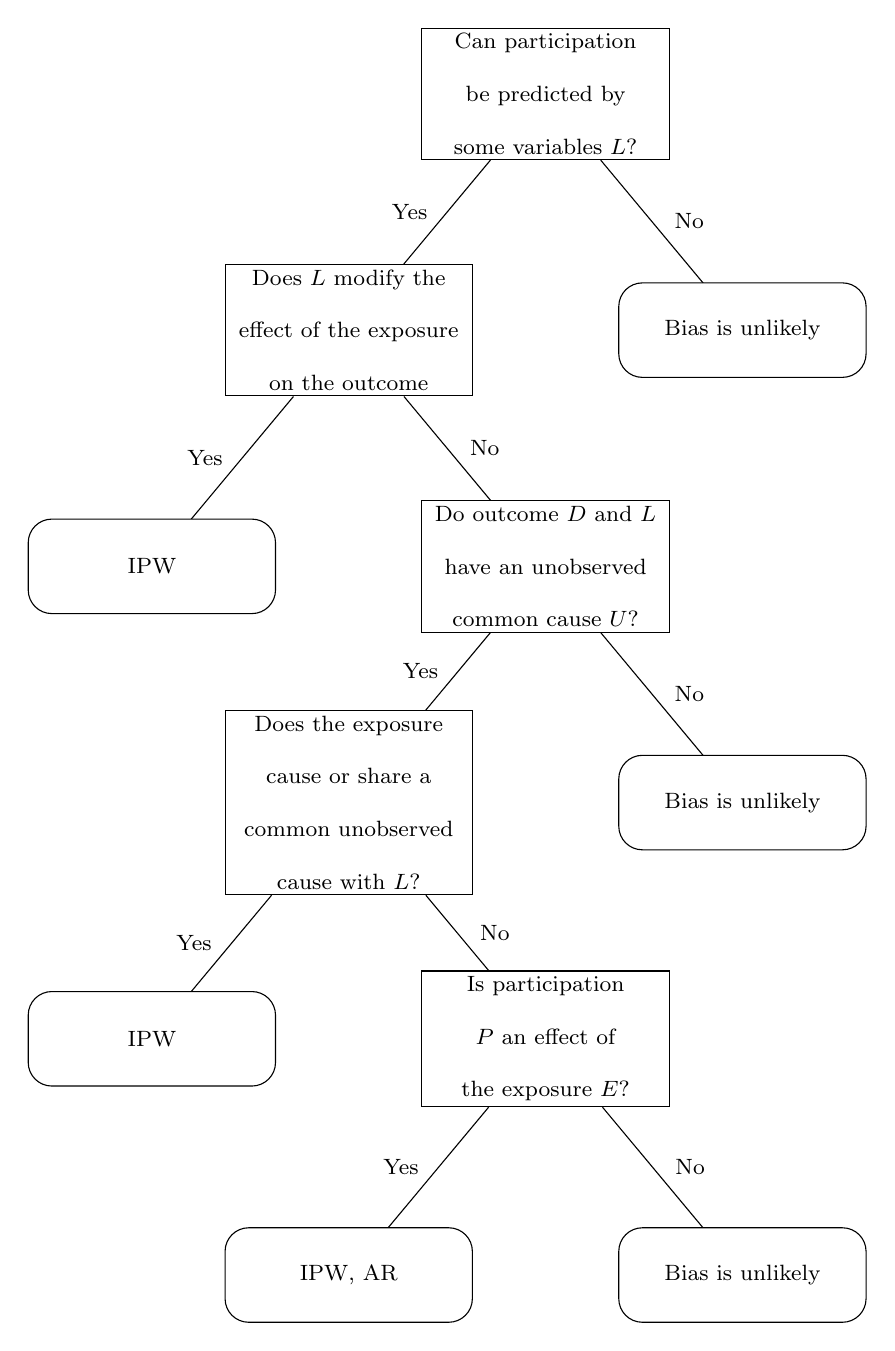
\begin{tikzpicture}
	[
	 sibling distance = 4cm,
	 level distance   = 3cm,
	 every node/.style = {shape=rectangle,
		                  draw,
		                  align=center,
		                  top color = white,
	                      font=\footnotesize,
	                      minimum size = 12mm,
	                      text width = 30mm,
	                      inner sep = 2pt
                         },
    L1/.style = {sibling distance=9cm},
    L2/.style = {sibling distance=5cm},
    L3/.style = {sibling distance=1cm},
    YN/.style = {minimum size = 8mm,
    	         text width = 8mm,
    	         pos = .5,
    	         text opacity = 1,
    	         fill opacity=0}
	]
	
	\newcommand{\LP}{Can participation be predicted by some variables $L$?}
	\newcommand{\nB}{Bias is unlikely}
	\newcommand{\LED}{Does $L$ modify the effect of the exposure
		on the outcome }
	\newcommand{\EL}{Does the exposure cause
		or share a common unobserved
		cause with $L$?}
	\newcommand{\EP}{Is participation $P$
		an effect of
		the exposure $E$?}
	\newcommand{\CCDL}{Do outcome $D$ and $L$
		have an unobserved
		common cause $U$?}	

	\node (A) {\LP}
	child [L2] {[] node  (B1) {\LED}
				child [L2] {[rounded corners=3mm] node (C1) {IPW}}
			    child [L2] {[] node (C2) {\CCDL}
		                    child [L2] {[] node (D1) {\EL}
		                    	        child [L2] {[rounded corners=3mm] node (E1) {IPW}}
		                    	        child [L2] {[] node (E2) {\EP}
		                    	        	        child [L2] {[rounded corners=3mm] node (F1) {IPW, AR}}
		                    	        	        child [L2] {[rounded corners=3mm] node (F2) {\nB}}
		                    	                                      }
		                                                  }
		                    child [L2] {[rounded corners=3mm] node (D2) {\nB}}                    
	                                         }}
	child [L2] {[rounded corners=3mm] node  (B2) {\nB}};
	
	 \begin{scope}[nodes = {draw = none}]
	   \path (A)  -- (B1) node [YN, left]   {Yes};
	   \path (A)  -- (B2) node [YN, right]  {No};
	   \path (B1) -- (C1) node [YN, left]   {Yes};
	   \path (B1) -- (C2) node [YN, right]  {No};
	   \path (C2) -- (D1) node [YN, left]   {Yes};
	   \path (C2) -- (D2) node [YN, right]  {No};
	   \path (D1) -- (E1) node [YN, left]   {Yes};
	   \path (D1) -- (E2) node [YN, right]  {No};
	   \path (E2) -- (F1) node [YN, left]   {Yes};
	   \path (E2) -- (F2) node [YN, right]  {No};
	 \end{scope}
\end{tikzpicture}}	
    \end{singlespace}
	
	%
\begin{tikzpicture}
	[
	 sibling distance = 4cm,
	 level distance   = 4cm,
	 every node/.style = {shape=rectangle,
		                  draw,
		                  align=center,
		                  top color = white,
	                      font=\footnotesize,
	                      minimum size = 22mm,
	                      text width = 28mm,
	                      inner sep = 0pt
                         },
    L1/.style ={sibling distance=9cm},
    L2/.style ={sibling distance=5cm},
    L3/.style ={sibling distance=3cm},
    YN/.style = {minimum size = 8mm,
    	text width = 8mm,
    	pos = .5,
    	text opacity = 1,
    	fill opacity=0}
	]
	
	\newcommand{\LP}{Is there a participation indicator $L$?}
	\newcommand{\nB}{Bias is unlikely}
	\newcommand{\LED}{Does $L$ modify the effect of the exposure
		             on the outcome }
	\newcommand{\EL}{Does the expo- sure cause
		             or share a common unobserved
		             cause with $L$?}
    \newcommand{\EP}{Is participation $P$
    	             an effect of
    	             the exposure $E$?}
    \newcommand{\CCDL}{Do outcome $D$ and $L$
    	               have an unobserved
    	               common cause $U$?}	
	\node (A) {\LP}
	child [L2] {[] node  (B1) {\LED}
				child [L1] {[] node (C1) {\EP}
					        child [L2] {[] node (Dx1) {\EL}
					        	        child [L2] {[] node (Ex1) {\CCDL}
					        	        	        child [L2] {[rounded corners=3mm] node (Fx1) {IPW}}
					        	        	        child [L2] {[rounded corners=3mm] node (Fx2) {MRP, IPW}}
					        	                                         }
					        	        child [L2] {[rounded corners=3mm] node (Ex2) {MRP, IPW}}
					                                       }
					        child [L2] {[rounded corners=3mm] node (Dx2) {MRP, IPW}}
				                              }
			    child [L1] {[] node (C2) {\CCDL}
		                    child [L2] {[] node (D1) {\EL}
		                    	        child [L2] {[rounded corners=3mm] node (E1) {IPW}}
		                    	        child [L2] {[] node (E2) {\EP}
		                    	        	        child [L2] {[rounded corners=3mm] node (F1) {AR, MRP, IPW}}
		                    	        	        child [L2] {[rounded corners=3mm] node (F2) {\nB}}
		                    	                                      }
		                                                  }
		                    child [L2] {[rounded corners=3mm] node (D2) {\nB}}                    
	                                         }}
	child [L2] {[rounded corners=3mm] node  (B2) {\nB}};
	
	 \begin{scope}[nodes = {draw = none}]
	   \path (A)  -- (B1) node [YN, left]   {Yes};
	   \path (A)  -- (B2) node [YN, right]  {No};
	   \path (B1) -- (C1) node [YN, left]   {Yes};
	   \path (B1) -- (C2) node [YN, right]  {No};
	   \path (C2) -- (D1) node [YN, left]   {Yes};
	   \path (C2) -- (D2) node [YN, right]  {No};
	   \path (D1) -- (E1) node [YN, left]   {Yes};
	   \path (D1) -- (E2) node [YN, right]  {No};
	   \path (E2) -- (F1) node [YN, left]   {Yes};
	   \path (E2) -- (F2) node [YN, right]  {No};
	   \path (Dx1) -- (Ex1) node [YN, left]   {Yes};
	   \path (Dx1) -- (Ex2) node [YN, right]  {No};
	   \path (C1) -- (Dx1) node [YN, left]   {Yes};
	   \path (C1) -- (Dx2) node [YN, right]  {No};
	   \path (Ex1) -- (Fx1) node [YN, left]   {Yes};
	   \path (Ex1) -- (Fx2) node [YN, right]  {No};
	 \end{scope}
\end{tikzpicture}
	\caption{Decision tree for identification of selection bias and choice of approach to correct for selection bias. See Figure \ref{fig:SelectionBias} for causal diagrams that underlie the decision tree. 
	To determine if selection bias is likely, and if so which correction method can be used, proceed through the questions from the top on. Ending in a node "Bias is unlikely" implies that a standard analysis without correction for selection bias will result in unbiased estimates. Otherwise, different correction types can be used, depending on the underlying causal structure. IPPW stands for analysis with inverse probability of participation weighting, AR for adjusted regression. For reasons of brevity, this decision tree does not isolate cases where multilevel regression and post stratification (MRP) can be used to correct bias. See appendix for a more detailed decision tree that represents also these cases.}
	\label{fig:DecisionTree}
\end{figure}


Structural analysis using directed acyclic graphs (DAGs) is a useful tool for the development of analysis strategies that remains underused. A practical argument against the use of DAGs is the uncertainty about hypothesized causal relationships. We proposed to use genetic correlation coefficients from LD score regression of publicly available GWAS summary statistics as one possibility to substantiate central assumptions about unobserved common causes. The main motivation to focus on common \emph{genetic} causes is the growing availability of GWAS summary statistics and methodological advances allowing estimation of heritability and genetic correlation coefficients from such statistics \cite{Bulik-Sullivan2015-er, Bulik-Sullivan2015-xn}. Because GWAS studies are association studies, they do not provide unambiguous proof for a causal role of genes. Still, even if GWAS associations estimates are partly driven by environmental factors, genetic correlation estimates from GWAS summary statistics are of interest because common environmental causes also contribute to the manifestation of selection bias.

A second challenge when using structural models is the difficulty of formulating DAGs for complex causal models \cite{Shrier2008-vr}. When judging the presence of bias due to self-selection and selective dropout, a simple decision tree can supplant the formulation of a complete DAG, so that researchers can determine the potential for selection bias by answering a sequence of questions about the relationship of participation predictors, exposures, and outcomes. Figure \ref{fig:DecisionTree} shows a decision tree that identifies when correction for bias is necessary, and what correction method is appropriate.

A topic closely related to selection bias is that of representativeness. While it was argued that representativeness can be detrimental to scientific inference, because understanding of mechanisms and careful control of relevant variables are central for this aim \cite{Rothman2013-qc}, others have emphasized the importance of representativeness---understood as the availability of weights for calculating valid population estimates \cite{Keiding2016-fv}. Careful experimentation based on hypothesized mechanisms is undoubtedly central to scientific progress. Still, this approach does not describe the often-exploratory analyses of cohort study data well. Moreover, if one understands causal inference as the central goal of scientific inquiry, ignoring non-representativeness of unweighted study samples does not only undermine generalization to the population of interest, but can also lead to incorrect scientific inferences by facilitating the "discovery" of associations where there are in fact none, or prevent the detection of existing associations.

In conclusion, self-selection into cohort studies and loss to follow up can lead to biased estimates of exposure outcome associations from large population based cohort studies. Structural analysis and empirical results suggest that especially for mental health related exposures and outcomes selection bias is likely. Still, the dependency of bias on the specific outcome, exposure, and study participation predictors makes general statements about selection bias for multi-exposure multi-outcome studies impossible. Instead, each  investigation of an exposure-outcome association has to assess selection bias. If bias is likely and valid participation predictors are available, weighting study participants by the inverse of their participation probability is a robust approach to control bias due to self-selection and loss to follow up.


Funding: This study was funded by the Norwegian Institute of Public Health.


Conflict of Interest: The authors declare that they have no conflict of interest.


\newpage

\printbibliography

\newpage

\processdelayedfloats

\clearpage

\makeatletter
\efloat@restorefloats
\makeatother

\appendix

\renewcommand{\thefigure}{S\arabic{figure}}
\renewcommand{\thepostfigure}{S\arabic{postfigure}}
\setcounter{figure}{0}
\setcounter{postfigure}{0}

\renewcommand{\thetable}{S\arabic{table}}
\renewcommand{\theposttable}{S\arabic{posttable}}
\setcounter{table}{0}
\setcounter{posttable}{0}

\phantomsection{Supplementary Information}
\setcounter{page}{1}

\phantomsection{Supplementary tables}


\begin{table}[ht]
	\begin{center}
		\begin{tabular}{llr}
			\hline
			Variable group        & Phenotype \& reference           & N \\
			\hline
			Participation         & Years education\cite{Okbay2016-mg} 	   & 292\,000\\
			predictors             & Age at first birth\cite{Barban2016-fa}       & 125\,000\\
			\multicolumn{1}{c}{"} & Nr. children born\cite{Barban2016-fa}       & 125\,000\\
			Exposure              & Birth weight\cite{Horikoshi2016-gz}    & 143\,000\\
			\multicolumn{1}{c}{"} & Ever smoked\cite{Tob_Gen_Cons2010-se} & 75\,000\\
			\multicolumn{1}{c}{"} & Nr. cigarettes per day\cite{Tob_Gen_Cons2010-se} & 75\,000\\
			\multicolumn{1}{c}{"} & Alcohol use\cite{Clarke2017-xz}       & 112\,000\\
			\multicolumn{1}{c}{"} & Lifetime cannabis use\cite{Stringer2016-or}     & 32\,000\\
			\multicolumn{1}{c}{"} & Substance abuse (ICD10 F10-F19)\cite{Canela-Xandri2017-xr}   & 408\,000\\
			\multicolumn{1}{c}{"} & Anxiety\cite{Otowa2016-uo}        & 31\,000\\
			\multicolumn{1}{c}{"} & Depressive symptoms\cite{Okbay2016-pj}        & 161\,000\\
			Outcome               & ADHD diagnosis\cite{Demontis2017-zu}     & 55\,000\\
			\hline
		\end{tabular}
	\end{center}
	\caption{Genome wide association studies on predictors of participation, exposures and outcome.}
	\label{tab:gwas}
\end{table}


% latex table generated in R 3.4.1 by xtable 1.8-2 package
% Fri Mar 23 14:45:43 2018
\setlength\tabcolsep{3pt}
\begin{longtable}{llrrrrrrrrr}
  \hline
p1 & p2 & $r_G$ & $se(r_G)$ & $z(r_G)$ & $h^2_{p2}$ & $se(h^2_{p2})$ & $z(h^2_{p2})$ & $h^2_{p1}$ & $se(h^2_{p1})$ & $z(h^2_{p1})$ \\ 
  \hline
  \endhead
ADHD & YearsEdu & -0.54 & 0.03 & -18.4 & 0.12 & 0.00 & 30.2 & 0.23 & 0.01 & 15.5 \\ 
  ADHD & AgeFirstBirth & -0.62 & 0.04 & -14.7 & 0.08 & 0.01 & 14.6 & 0.23 & 0.01 & 15.5 \\ 
  ADHD & NumChildrBorn & 0.36 & 0.07 & 5.3 & 0.03 & 0.00 & 9.9 & 0.23 & 0.01 & 15.5 \\ 
  ADHD & BirthWeight & -0.14 & 0.04 & -3.6 & 0.13 & 0.01 & 15.7 & 0.23 & 0.01 & 15.5 \\ 
  ADHD & EverSmoked & 0.49 & 0.06 & 7.9 & 0.08 & 0.01 & 11.4 & 0.23 & 0.01 & 15.5 \\ 
  ADHD & CigPerDay & 0.41 & 0.10 & 4.2 & 0.03 & 0.01 & 4.3 & 0.23 & 0.01 & 15.5 \\ 
  ADHD & AlcUse & -0.04 & 0.05 & -0.8 & 0.08 & 0.01 & 13.0 & 0.23 & 0.01 & 15.5 \\ 
  ADHD & DeprSymp & 0.45 & 0.05 & 8.5 & 0.05 & 0.00 & 12.8 & 0.23 & 0.01 & 15.5 \\ 
  ADHD & Anxiety & 0.27 & 0.14 & 1.9 & 0.06 & 0.03 & 2.5 & 0.23 & 0.01 & 15.5 \\ 
  ADHD & Cannabis & 0.32 & 0.07 & 4.5 & 0.09 & 0.02 & 5.5 & 0.23 & 0.01 & 15.5 \\ 
  YearsEdu & AgeFirstBirth & 0.72 & 0.03 & 27.9 & 0.08 & 0.01 & 14.6 & 0.12 & 0.00 & 30.2 \\ 
  YearsEdu & NumChildrBorn & -0.23 & 0.04 & -6.0 & 0.03 & 0.00 & 9.9 & 0.12 & 0.00 & 30.2 \\ 
  YearsEdu & EverSmoked & -0.35 & 0.04 & -9.1 & 0.08 & 0.01 & 11.4 & 0.12 & 0.00 & 30.2 \\ 
  NumChildrBorn & AgeFirstBirth & -0.65 & 0.05 & -13.6 & 0.08 & 0.01 & 14.6 & 0.03 & 0.00 & 9.9 \\ 
  BirthWeight & YearsEdu & 0.11 & 0.03 & 4.3 & 0.12 & 0.00 & 30.2 & 0.13 & 0.01 & 15.7 \\ 
  BirthWeight & AgeFirstBirth & 0.10 & 0.04 & 2.5 & 0.08 & 0.01 & 14.6 & 0.13 & 0.01 & 15.7 \\ 
  BirthWeight & NumChildrBorn & -0.03 & 0.05 & -0.5 & 0.03 & 0.00 & 9.9 & 0.13 & 0.01 & 15.7 \\ 
  BirthWeight & EverSmoked & 0.01 & 0.04 & 0.1 & 0.08 & 0.01 & 11.4 & 0.13 & 0.01 & 15.7 \\ 
  BirthWeight & DeprSymp & -0.07 & 0.04 & -1.7 & 0.05 & 0.00 & 12.8 & 0.13 & 0.01 & 15.7 \\ 
  BirthWeight & Anxiety & -0.07 & 0.11 & -0.7 & 0.06 & 0.03 & 2.5 & 0.13 & 0.01 & 15.7 \\ 
  EverSmoked & AgeFirstBirth & -0.37 & 0.05 & -7.3 & 0.08 & 0.01 & 14.6 & 0.08 & 0.01 & 11.4 \\ 
  EverSmoked & NumChildrBorn & 0.08 & 0.07 & 1.3 & 0.03 & 0.00 & 9.9 & 0.08 & 0.01 & 11.4 \\ 
  CigPerDay & YearsEdu & -0.26 & 0.06 & -4.3 & 0.12 & 0.00 & 30.2 & 0.03 & 0.01 & 4.3 \\ 
  CigPerDay & AgeFirstBirth & -0.46 & 0.10 & -4.6 & 0.08 & 0.01 & 14.6 & 0.03 & 0.01 & 4.3 \\ 
  CigPerDay & NumChildrBorn & 0.16 & 0.10 & 1.5 & 0.03 & 0.00 & 9.9 & 0.03 & 0.01 & 4.3 \\ 
  CigPerDay & BirthWeight & -0.04 & 0.06 & -0.7 & 0.13 & 0.01 & 15.7 & 0.03 & 0.01 & 4.3 \\ 
  CigPerDay & EverSmoked & 0.37 & 0.11 & 3.5 & 0.08 & 0.01 & 11.4 & 0.03 & 0.01 & 4.3 \\ 
  CigPerDay & DeprSymp & 0.26 & 0.09 & 3.0 & 0.05 & 0.00 & 12.8 & 0.03 & 0.01 & 4.3 \\ 
  CigPerDay & Anxiety & -0.03 & 0.20 & -0.2 & 0.06 & 0.03 & 2.5 & 0.03 & 0.01 & 4.3 \\ 
  AlcUse & YearsEdu & 0.18 & 0.03 & 5.9 & 0.12 & 0.00 & 30.2 & 0.08 & 0.01 & 13.0 \\ 
  AlcUse & AgeFirstBirth & 0.11 & 0.05 & 2.3 & 0.08 & 0.01 & 14.6 & 0.08 & 0.01 & 13.0 \\ 
  AlcUse & NumChildrBorn & 0.06 & 0.06 & 1.0 & 0.03 & 0.00 & 9.9 & 0.08 & 0.01 & 13.0 \\ 
  AlcUse & BirthWeight & -0.06 & 0.04 & -1.3 & 0.13 & 0.01 & 15.7 & 0.08 & 0.01 & 13.0 \\ 
  AlcUse & EverSmoked & 0.40 & 0.06 & 6.3 & 0.08 & 0.01 & 11.4 & 0.08 & 0.01 & 13.0 \\ 
  AlcUse & CigPerDay & -0.10 & 0.09 & -1.1 & 0.03 & 0.01 & 4.3 & 0.08 & 0.01 & 13.0 \\ 
  AlcUse & DeprSymp & -0.16 & 0.06 & -2.8 & 0.05 & 0.00 & 12.8 & 0.08 & 0.01 & 13.0 \\ 
  AlcUse & Anxiety & 0.05 & 0.12 & 0.4 & 0.06 & 0.03 & 2.5 & 0.08 & 0.01 & 13.0 \\ 
  AlcUse & Cannabis & 0.39 & 0.08 & 4.8 & 0.09 & 0.02 & 5.5 & 0.08 & 0.01 & 13.0 \\ 
  DeprSymp & YearsEdu & -0.33 & 0.04 & -9.0 & 0.12 & 0.00 & 30.2 & 0.05 & 0.00 & 12.8 \\ 
  DeprSymp & AgeFirstBirth & -0.34 & 0.05 & -7.4 & 0.08 & 0.01 & 14.6 & 0.05 & 0.00 & 12.8 \\ 
  DeprSymp & NumChildrBorn & 0.19 & 0.07 & 2.9 & 0.03 & 0.00 & 9.9 & 0.05 & 0.00 & 12.8 \\ 
  DeprSymp & EverSmoked & 0.25 & 0.06 & 4.4 & 0.08 & 0.01 & 11.4 & 0.05 & 0.00 & 12.8 \\ 
  Anxiety & YearsEdu & -0.31 & 0.09 & -3.5 & 0.12 & 0.00 & 30.2 & 0.06 & 0.03 & 2.5 \\ 
  Anxiety & AgeFirstBirth & -0.24 & 0.12 & -2.0 & 0.08 & 0.01 & 14.6 & 0.06 & 0.03 & 2.5 \\ 
  Anxiety & NumChildrBorn & 0.20 & 0.17 & 1.2 & 0.03 & 0.00 & 9.9 & 0.06 & 0.03 & 2.5 \\ 
  Anxiety & EverSmoked & 0.58 & 0.16 & 3.5 & 0.08 & 0.01 & 11.4 & 0.06 & 0.03 & 2.5 \\ 
  Anxiety & DeprSymp & 0.65 & 0.17 & 3.9 & 0.05 & 0.00 & 12.8 & 0.06 & 0.03 & 2.5 \\ 
  Cannabis & YearsEdu & -0.04 & 0.05 & -0.9 & 0.12 & 0.00 & 30.2 & 0.09 & 0.02 & 5.5 \\ 
  Cannabis & AgeFirstBirth & -0.17 & 0.07 & -2.4 & 0.08 & 0.01 & 14.6 & 0.09 & 0.02 & 5.5 \\ 
  Cannabis & NumChildrBorn & 0.05 & 0.10 & 0.5 & 0.03 & 0.00 & 9.9 & 0.09 & 0.02 & 5.5 \\ 
  Cannabis & BirthWeight & -0.02 & 0.07 & -0.3 & 0.13 & 0.01 & 15.7 & 0.09 & 0.02 & 5.5 \\ 
  Cannabis & EverSmoked & 0.68 & 0.10 & 6.5 & 0.08 & 0.01 & 11.4 & 0.09 & 0.02 & 5.5 \\ 
  Cannabis & CigPerDay & 0.07 & 0.13 & 0.6 & 0.03 & 0.01 & 4.3 & 0.09 & 0.02 & 5.5 \\ 
  Cannabis & DeprSymp & 0.25 & 0.08 & 2.9 & 0.05 & 0.00 & 12.8 & 0.09 & 0.02 & 5.5 \\ 
  Cannabis & Anxiety & -0.05 & 0.18 & -0.3 & 0.06 & 0.03 & 2.5 & 0.09 & 0.02 & 5.5 \\ 
  \hline
\caption{SNP based genetic correlations and heritability estimates.} 
\label{tab:rg}
\end{longtable}


\newpage

\phantomsection{Supplementary figures}

\begin{figure}[ht]
	\caption{}
	\label{fig:covariation}
\end{figure}

\begin{figure}[ht]
	\caption{}
	\label{fig:IPW}
\end{figure}

\begin{figure}[ht]
	\caption{} 
	\label{fig:logRRs}
\end{figure}

\begin{figure}[ht]
	\caption{}
	\label{fig:ropeplots}
\end{figure}


\end{document}
